\documentclass[12pt,a4paper,openright,twoside]{book}
\usepackage[utf8]{inputenc}
\usepackage{disi-thesis}
\usepackage{code-lstlistings}
\usepackage{notes}
\usepackage{shortcuts}
\usepackage{acronym}
\usepackage{float}
\usepackage{algorithm}
\usepackage{algorithmicx}
\usepackage{algpseudocode}
\usepackage{amsmath}
\usepackage{amsfonts}



\school{\unibo}
\programme{Corso di Laurea Magistrale in Ingegneria e Scienze Informatiche}
\title{Fancy Title}
\author{Lorenzo Gardini}
\date{\today}
\subject{Supervisor's course name}
\supervisor{Matteo Golfarelli}
\session{2}
\academicyear{2025-2026}

% Definition of acronyms
\acrodef{IoT}{Internet of Thing}
\acrodef{vm}[VM]{Virtual Machine}


\mainlinespacing{1.241} % line spacing in mainmatter, comment to default (1)

\begin{document}

\frontmatter\frontispiece

\begin{abstract}	
Max 2000 characters, strict.
\end{abstract}

\begin{dedication} % this is optional
Optional. Max a few lines.
\end{dedication}

%----------------------------------------------------------------------------------------
\tableofcontents   
\listoffigures     % (optional) comment if empty
\lstlistoflistings % (optional) comment if empty
%----------------------------------------------------------------------------------------

\mainmatter

%----------------------------------------------------------------------------------------
% \chapter{Introduzione}

I sistemi di \textit{recommendation} sono elementi fondamentali in molti settori legati alla vita quotidiana, come l'e-commerce, i social network e i servizi di streaming, dove la personalizzazione dei contenuti è volta al miglioramento dell'esperienza dell'utente. L'efficacia di questi sistemi è strettamente legata alla disponibilità e al volume crescente dei dati che, se opportunamente sfruttati, possono migliorare la qualità delle raccomandazioni.

Nella prima parte di questa tesi si fornirà una panoramica generale su questi sistemi, esplorando i principali approcci e le tecniche impiegate per realizzare modelli di raccomandazione efficaci. Si tratteranno i modelli basati su feedback espliciti e impliciti, esaminando le caratteristiche e le differenze tra i due tipi di dati. Successivamente, si approfondiranno alcuni algoritmi specifici, esplorando i loro vantaggi, svantaggi e le loro applicazioni in vari contesti.

La seconda parte della tesi viene descritta la parte inerente al lavoro svolto durante il mio tirocinio, in cui mi sono concentrato sulla creazione di un'interfaccia utente che facilitasse la creazione, il testing e l'utilizzo modelli di raccomandazione. Nello specifico, ho lavorato sul wrapping delle interfacce dei modelli di librerie popolari come Surprise, LightFM e Implicit, con l’obiettivo di rispettare i vincoli specifici imposti dalla mia azienda. Verranno discusse le sfide affrontate, le soluzioni adottate e i risultati ottenuti.

Il contributo di questa tesi si inserisce nel contesto della crescente necessità di rendere i sistemi di raccomandazione sempre più accessibili e facilmente integrabili in ambienti di lavoro aziendali, dove personalizzazione ed efficienza sono essenziali.

% \chapter{La recommendation}

\section{Introduzione}

Come fa \textit{Spotify} a sapere quale canzone potresti voler ascoltare? E come fa \textit{Netflix} a suggerirti la prossima serie da guardare? Questo è possibile grazie al modello di \textit{recommendation} basato su \textit{machine learning} che analizza cosa piace all'utente e gli propone contenuti su misura. Di solito si utilizzano due tipi principali di raccomandazioni:

\begin{itemize}
    \item per la \textit{home page}: i consigli sono personalizzati per un utente in base ai suoi interessi. Ogni utente vede consigli diversi
    \item su articoli correlati: sono consigli simili a un di un articolo specifico. Per esempio in Google Play, gli utenti che visualizzano la pagina di un'app di matematica potrebbero vedere anche un riquadro con app correlate, come altre app di matematica o di scienze
\end{itemize}

Un sistema di \textit{recommendation} aiuta gli utenti a scoprire contenuti interessanti all'interno di un'enorme quantità di dati. Per esempio su YouTube ci sono miliardi di video, con nuovi contenuti che vengono aggiunti ogni giorno. Come può un utente trovare qualcosa di nuovo che valga la pena guardare o provare? La ricerca manuale è un'opzione. Tuttavia, un motore di raccomandazione è in grado di suggerire contenuti che magari l'utente non avrebbe mai pensato di cercare da solo. Basti sapere che, secondo quanto dice \textit{Google}:

\begin{itemize}
    \item il 40\% delle app installate dal \textit{Google Play} derivano da raccomandazioni
    \item il 60\% del tempo di visualizzazione su \textit{YouTube} proviene dalle raccomandazioni
\end{itemize}


\subsubsection{Terminologia}
Ci sono alcuni termini da introdurre:

\begin{itemize}
    \item \textit{item}: sono gli elementi/entità consigliate dal sistema. Su \textit{Spotify} sono le canzoni, su \textit{Amazon} sono i prodotti, su \textit{Intragram} sono i \textit{post}
    \item \textit{query}: sono le informazioni utilizzate da un sistema per fornire consigli. Le \textit{query} possono essere una combinazione di informazioni dell'utente (e.g. ID, elementi con i quali ha interagito in passato etc.) e contesto aggiuntivo (e.g. ora del giorno, per quanto tempo ha osservato quel prodotto o quell'episodio etc.)
\end{itemize}

I passaggi tipici che ti utilizzano sono: 

\begin{enumerate}
    \item generazione dei candidati: il sistema parte da un corpus di \textit{item}, potenzialmente enorme, e ne estrae un sottoinsieme molto più piccolo di candidati
    \item calcolo dello \textit{score}: un altro modello, più preciso del primo dato che lavora su una quantità molto minore di dati, assegna un punteggio ai candidati
    \item \textit{re-ranking}: i candidati vengono ordinati per lo score ricevuto considerando eventuali ulteriori vincoli (e.g. rimuovendo contenuti che l'utente ha segnalato come non graditi, oppure aumentare il punteggio di contenuti più recenti). Il riordinamento può garantire maggiore varietà, attualità e imparzialità.
\end{enumerate}

\section{Generazione dei candidati}\label{generazione_dei_candidati}

\subsubsection{Embedding}

Gli \textit{item} e le \textit{query} vengono mappati su  vettore di \textit{embedding} in uno spazio comune $E = \mathbb{R}^k$. Normalmente lo spazio di \textit{embedding} ha una dimensione molto più piccola rispetto alla grandezza del corpus e cattura alcune strutture latenti dell'insieme di \textit{item} o \textit{query}. Gli elementi tra loro simili finiscono per essere vicini nello spazio di \textit{embedding}. Il concetto di ``vicinanza" è definito da una misura di similarità.
 
\subsubsection{Calcolo della similarità}

Una misura di similarità è una funzione $s: E \times E \to \mathbb{R}$ che prende in input una coppia di vettori di \textit{embedding} e restituisce un valore scalare che ne misura la similarità. Gli \textit{embedding} possono essere utilizzati per la generazione dei candidati come segue: dato un vettore di \textit{embedding} per una query $q \in E$, il sistema cerca gli \textit{embedding} degli elementi $x \in E$ che sono vicini a $q$, ossia, gli \textit{embedding} con una similarità elevata.

Per determinare il grado di similarità, la maggior parte dei sistemi di \textit{recommendation} si basa su una o più delle seguenti misure:

\begin{itemize}
    \item coseno: semplicemente il coseno dell'angolo tra i due vettori $s(q, x) = cos(q, x)$
    \item prodotto scalare: è dato da: $s(q, x) = \langle q, x \rangle = \sum\limits_{i=1}^{d} q_i x_i$. È anche dato da $s(q, x) = \|x\| \|q\| \cos(q, x)$ che corrisponde al coseno dell'angolo moltiplicato per il prodotto delle norme. Pertanto, se gli \textit{embedding} sono normalizzati, il prodotto scalare e il coseno coincidono    
    \item distanza euclidea: questa è la distanza usuale nello spazio euclideo $s(q, x) = \|q - x\| = \left[ \sum\limits_{i=1}^{d} (q_i - x_i)^2 \right]^{\frac{1}{2}}$. Una distanza minore indica una similarità maggiore. Da notare che, quando gli \textit{embedding} sono normalizzati, la distanza euclidea al quadrato coincide con il prodotto scalare (e il coseno) fino a una costante, poiché in quel caso $\frac{1}{2} \|q - x\|^2 = 1 - \langle q, x \rangle$
\end{itemize}


\begin{figure}[H]
    \centering
    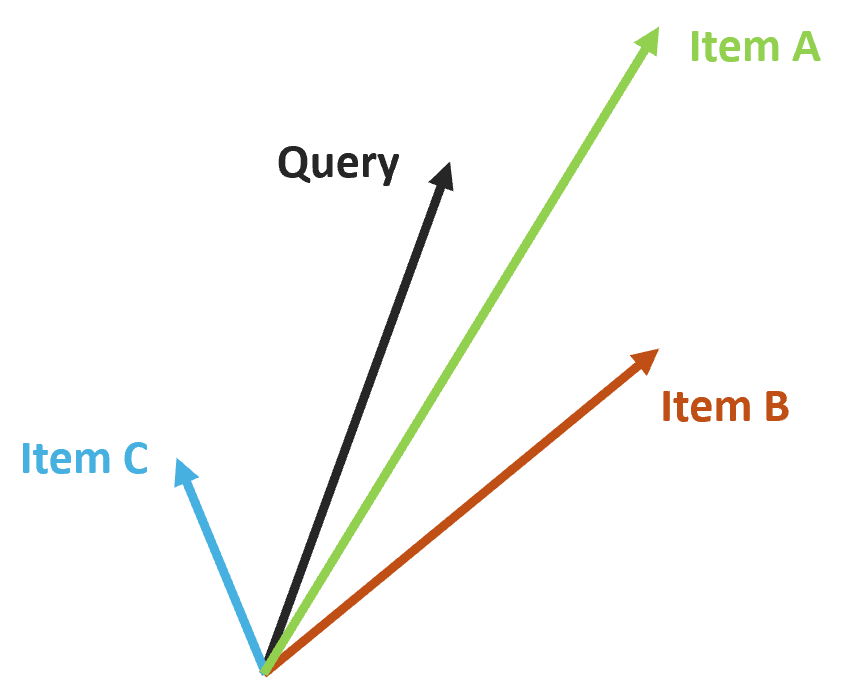
\includegraphics[scale=0.8]{figures/embedding.PNG}
    \caption{Il vettore nero illustra l'\textit{embedding} della query. Gli altri tre vettori di \textit{embedding} (\textit{Item A}, \textit{Item B}, \textit{Item C}) rappresentano gli \text{item} candidati. A seconda della misura di similarità utilizzata, la classifica degli elementi può essere diversa}
    \label{fig:embedding}
\end{figure}

Rispetto al coseno, la similarità del prodotto scalare è sensibile alla norma dell'\textit{embedding}. Cioè, maggiore è la norma di un \textit{embedding}, maggiore sarà la similarità e più è probabile che l'\textit{item} venga raccomandato. Questo può influenzare le raccomandazioni nei seguenti modi:

\begin{itemize}
    \item gli elementi che appaiono molto frequentemente nel \textit{training set} (ad esempio, le top canzoni italiane del momento su \textit{Spotify}) tendono ad avere \textit{embedding} con norme grandi. Se è desiderabile catturare informazioni sulla popolarità, allora si dovrebbe preferire il prodotto scalare. Tuttavia, se non si presta attenzione, gli elementi popolari potrebbero finire per dominare le raccomandazioni. In pratica, si possono utilizzare altre varianti delle misure di similarità che pongono meno enfasi sulla norma dell'\textit{item}. Ad esempio, definire $s(q, x) = \|q\|^{\alpha} \|x\|^{\alpha} \cos(q, x)$ per qualche $\alpha \in (0,1)$
    \item Gli elementi che appaiono molto raramente potrebbero non essere aggiornati frequentemente durante l'addestramento. Di conseguenza, se vengono inizializzati con una norma elevata, il sistema potrebbe raccomandare elementi rari invece di quelli più rilevanti. Per evitare questo problema, prestare attenzione all'inizializzazione degli \textit{embedding} e utilizzare una regolarizzazione appropriata
\end{itemize}


Le due tecniche più comuni per la generazione dei candidati sono:

\begin{itemize}
    \item \textit{content-based filtering}
    \item \textit{collaborative filtering}
\end{itemize}
  
\section{Content-based filtering}
Il \textit{content-based filtering} utilizza la similarità tra gli oggetti per raccomandare elementi simili a quelli che l'utente apprezza o ha apprezzato. Ad esempio, se l'utente $A$ guarda due film \textit{fantasy}, il sistema può raccomandargli altri film dello stesso genere.

L'idea è che se ad un utente è piaciuto un certo \textit{item} con certe caratteristiche, il sistema proporrà altri \textit{item} simili per contenuto.

Per prima cosa si crea un profilo degli \textit{item}, cioè viene rappresentato tramite un insieme di caratteristiche (\textit{feature}). Per un film, per esempio, si possono utilizzare il/i generi, gli attori principali, l'anno di uscita, la durata etc.

Dopodiché si costruisce un profilo dell'utente analizzando gli oggetti che ha valutato positivamente. Il profilo rappresenta una media delle caratteristiche degli oggetti preferiti.

Si confronta il profilo dell'utente con gli \textit{item} non ancora visti usando una metrica di similarità (es. coseno, distanza euclidea~\ref{generazione_dei_candidati}).

vengono raccomandati gli \textit{item} più simili al profilo dell'utente.

\subsubsection{Esempio}

Si supponga che all'utente $A$ siano piaciuti due film:

\begin{itemize}
    \item \textit{Matrix} i cui generi sono \textit{Azione} e \textit{Fantascienza}
    \item \textit{Inception} i cui generi sono \textit{Azione}, \textit{Fantascienza} e \textit{Thriller}
\end{itemize}

Si crea il profilo dell'utente con la media delle caratteristiche: 

\begin{itemize}
    \item \textit{Azione} $= 1$
    \item \textit{Fantascienza} $= 1$
    \item \textit{Thriller} $= 0.5$
\end{itemize}

Poi si selezionano altri film dal catalogo, ad esempio:

\begin{itemize}
    \item \textit{Interstellar} i cui generi sono \textit{Fantascienza} e \textit{Drammatico}
    \item \textit{John Wick} il cui genere è \textit{Azione}
\end{itemize}

\begin{figure}[H]
    \centering
    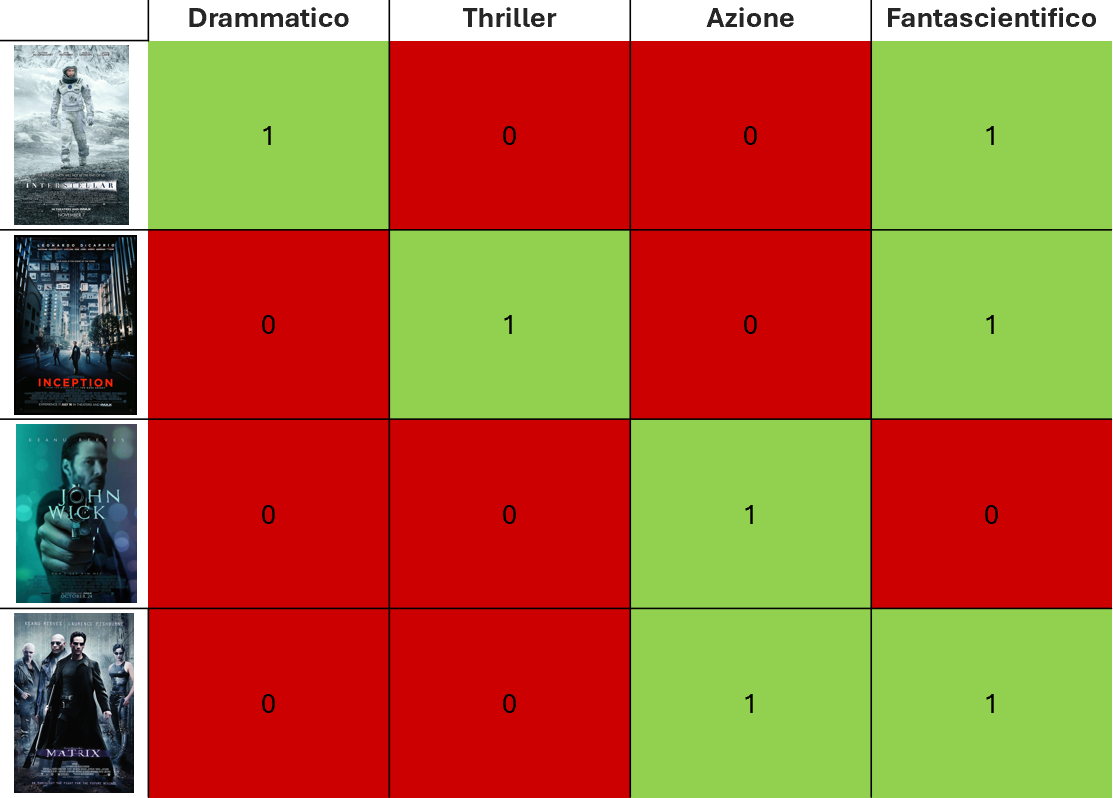
\includegraphics[scale=0.5]{figures/content_based_filtering.PNG}
    \caption{La figura mostra i vettori delle caratteristiche dei film (in questo caso il genere) per i film in esempio. Se il film appartiene ad uno specifico genere viene posto il valore $1$, altrimenti $0$}
    \label{fig:item_vector}
\end{figure}

Si creano vettori per i film considerando tutti i generi analizzati fino ad ora e si calcola la similarità con il profilo dell'utente. Si ottiene, utilizzando per esempio la similarità coseno, un valore di $0.47$ per $Interstellar$ e di $0.67$ per \textit{John Wick}, quindi quest'ultimo viene raccomandato prima di \textit{Interstellar}, perché è più simile al profilo dell'utente.


\subsubsection{Vantaggi e svantaggi}

I vantaggi di quest'approccio sono:
\begin{itemize}
    \item il modello non ha bisogno di dati su altri utenti, poiché le raccomandazioni sono specifiche per questo utente. questo lo rende più facile da scalare a un grande numero di utenti
    \item il modello può catturare gli interessi specifici di un utente e può raccomandare \textit{item} di nicchia che interessano a pochissimi altri utenti
\end{itemize}

Gli svantaggi di quest'approccio sono:
\begin{itemize}
    \item poiché la rappresentazione delle caratteristiche degli oggetti è in parte progettata manualmente, questa tecnica richiede molta conoscenza del dominio. Il modello può essere solo quindi valido quanto le caratteristiche progettate manualmente
    \item il modello può fare raccomandazioni solo basate sugli interessi esistenti dell'utente. In altre parole, ha una capacità limitata di espandere gli interessi dell'utente
\end{itemize}

\section{Collaborative filtering}

Per affrontare alcune delle limitazioni del \textit{content-base filtering}, il \textit{collaborative filtering} utilizza simultaneamente le somiglianze tra utenti e \textit{item} per fornire raccomandazioni. I modelli possono raccomandare un \textit{item} all'utente $A$ in base agli interessi di un utente simile $B$ anche se $A$ non ha mai visto \textit{item} simili. Inoltre, gli \textit{embedding} possono essere appresi automaticamente, senza dover progettare manualmente le caratteristiche.

Si consideri un sistema di raccomandazione di film in cui i dati di addestramento consistono in una matrice di feedback in cui:

\begin{itemize}
    \item Ogni riga rappresenta un utente.
    \item Ogni colonna rappresenta un \textit{item} (un film).
    \item Il feedback sui film rientra in una delle due categorie:
    \begin{itemize}
        \item esplicito: gli utenti specificano quanto gli è piaciuto un determinato film fornendo una valutazione numerica.
        \item implicito: se un utente guarda un film, il sistema deduce che l'utente è interessato.
    \end{itemize}
\end{itemize}

Per semplificare, si supponga che la matrice di feedback sia binaria; cioè, un valore di $1$ indica interesse per il film.

Quando un utente visita la homepage, il sistema dovrebbe raccomandare film basati su:

\begin{enumerate}
    \item somiglianza con i film che l'utente ha apprezzato in passato
    \item film che utenti simili hanno apprezzato
\end{enumerate}

\subsubsection{1D embedding}

Si assegna a ciascun film uno scalare in $[-1, 1]$ che descriva se il film è destinato a bambini (valori negativi) o ad adulti (valori positivi). Allo stesso modo, per ciascun utente si assegna uno scalare in $[-1, 1]$ che descriva il suo interesse per i film per bambini o per adulti. Il prodotto dell'\textit{embedding} del film e dell'\textit{embedding} dell'utente dovrebbe essere più alto (vicino a 1) per i film che dovrebbero piacere all'utente.

\begin{figure}[H]
    \centering
    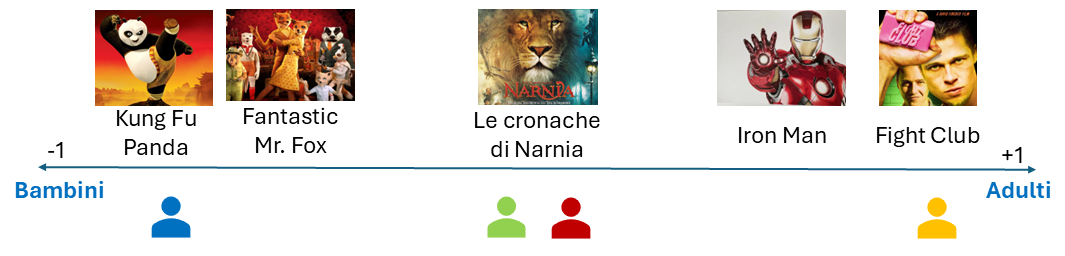
\includegraphics[scale=0.4]{figures/collaborative_filtering/embeddings.PNG}
    \caption{Rappresentazione su un asse 1D delle posizioni di utenti e film rispetto allo scalare assegnato nell'intervallo $[-1, 1]$}
    \label{fig:embeddings}
\end{figure}

Nella seguente matrice, ogni segno di spunta identifica un film che un determinato utente ha guardato. Il terzo e il quarto utente hanno preferenze evidenti per questa caratteristica: il terzo utente preferisce i film per bambini, mentre il quarto preferisce i film per adulti. Ciò non vale invece per il primo e del secondo utente.

\begin{figure}[H]
    \centering
    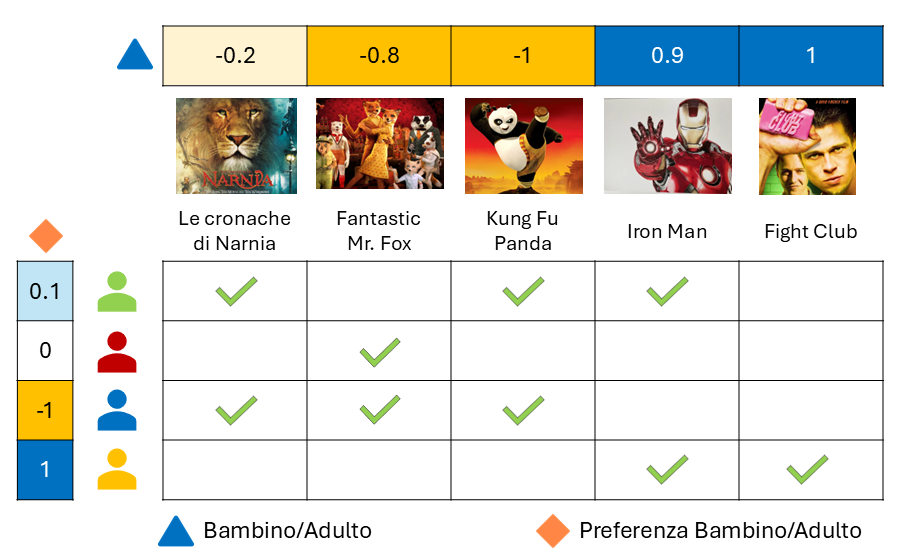
\includegraphics[scale=0.5]{figures/collaborative_filtering/1D_matrix.PNG}
    \caption{matrice che mostra i film guardati dagli utenti, le categorie dei film e le preferenze degli utenti}
    \label{fig:1D_matrix}
\end{figure}

\subsubsection{2D embedding}

Una sola caratteristica non è sufficiente a spiegare le preferenze di tutti gli utenti. Per superare questo problema, si utilizza una seconda caratteristica: il grado in cui ogni film è un \textit{blockbuster} (film molto popolare e di grande successo al botteghino) o un film d'autore. Con una seconda caratteristica, ora si può rappresentare ogni film con il seguente \textit{embedding} bidimensionale:

\begin{figure}[H]
    \centering
    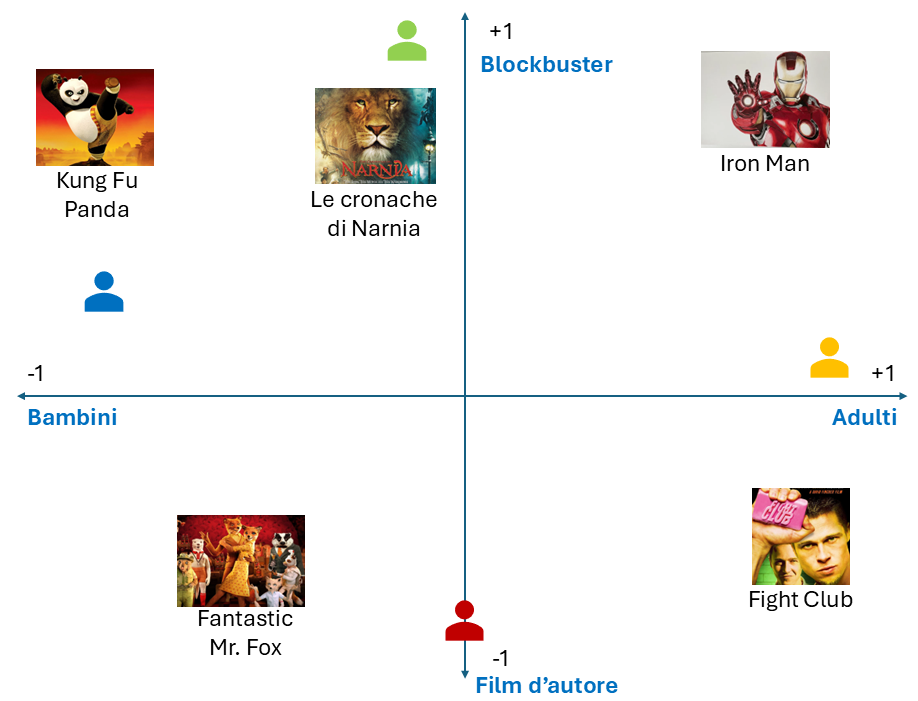
\includegraphics[scale=0.4]{figures/collaborative_filtering/axes.PNG}
    \caption{gli assi mostrano, per ciascuna caratteristica, la posizione dei film e le preferenze degli utenti}
    \label{fig:embedding_axes}
\end{figure}

Nel grafico sono rappresentati sia gli elementi che gli utenti nello stesso spazio di \textit{embedding}. Questo perché si può pensare allo spazio di \textit{embedding} come a una rappresentazione astratta comune sia agli \textit{item} che agli utenti, in cui si può misurare la similarità.

\begin{figure}[H]
    \centering
    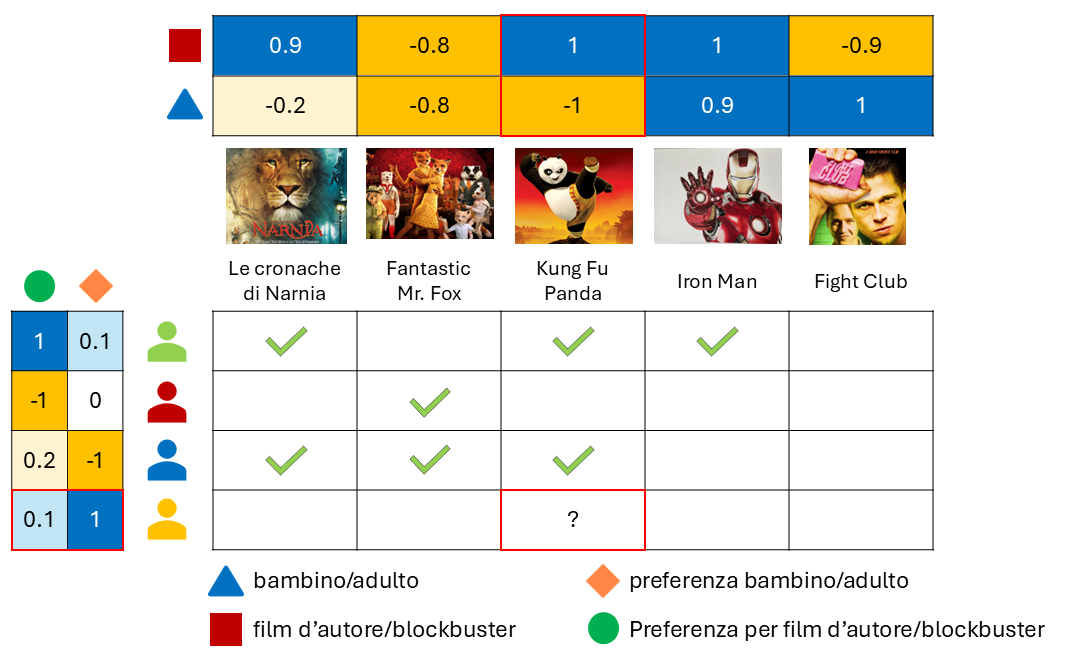
\includegraphics[scale=0.4]{figures/collaborative_filtering/2D_matrix.PNG}
    \caption{matrice che mostra i film guardati dagli utenti, le categorie dei film e le preferenze degli utenti estese}
    \label{fig:2D_matrix}
\end{figure}

L'obbiettivo è che per ogni coppia (utente, \textit{item}) il prodotto scalare dell'\textit{embedding} dell'utente e dell'\textit{embedding} dell'\textit{item} fosse vicino a $1$ quando l'utente ha guardato il film e a $0$ in caso contrario.

I modelli apprendono automaticamente un vettore di \textit{embedding} per ciascun utente che spieghi al meglio le sue preferenze. Di conseguenza, gli \textit{embedding} di utenti con gusti simili risulteranno vicini tra loro. Allo stesso modo il modello apprende gli \textit{embedding} dei film in modo da spiegare al meglio la matrice di feedback. Anche in questo caso, gli \textit{embedding} dei film apprezzati da utenti simili saranno vicini nello spazio degli embedding.

\subsubsection{Vantaggi e svantaggi}

I vantaggi di quest'approccio sono:

\begin{itemize}
  \item non è necessaria conoscenza del dominio: gli embedding vengono appresi automaticamente
  \item serendipità: anche se il modello non sa che l'utente è interessato a un determinato \textit{item} potrebbe comunque raccomandarlo perché utenti simili sono interessati a quell'\textit{item}
  \item ottimo punto di partenza: il sistema ha bisogno solo della matrice di feedback, e non di informazioni contestuali, per addestrare un modello
\end{itemize}

Gli svantaggi di quest'approccio sono:

\begin{itemize}
  \item non si può gestire \textit{item} nuovi: se un oggetto non è stato visto durante l'addestramento, il sistema non può creare un \textit{embedding} per esso. Questo problema è noto come \textit{cold-start}. Tuttavia, esistono tecniche che possono affrontare in parte questo problema: 

  \begin{itemize}
    \item proiezione: dato un nuovo \textit{item} $i_0$ non visto durante l'addestramento, se il sistema ha alcune interazioni con utenti, può facilmente calcolare un \textit{embedding} per quell'\textit{item} senza riaddestrare l'intero modello. Basta risolvere la seguente equazione (o la sua versione pesata):

    \[
    \min_x \sum_{i}(r_{ui} - x^T u_i)^2
    \]

    Gli \textit{embedding} dell'utente vengono mantenuti fissi, e il sistema risolve per ottenere l'\textit{embedding} dell'\textit{item}. Lo stesso approccio può essere utilizzato per un nuovo utente.
    \item euristiche: se il sistema non ha interazioni, può approssimare l'\textit{embedding} di un \textit{item} facendo la media degli \textit{embedding} di \textit{item} appartenenti alla stessa categoria
  \end{itemize}

  \item difficoltà nell'includere caratteristiche aggiuntive per \textit{query}/\textit{item}: le caratteristiche aggiuntive (\textit{side features}) sono tutte quelle informazioni oltre all'ID della query o dell'\text{item}. Per esempio, per i film, le caratteristiche possono includere il paese o l'età. Includere queste caratteristiche migliora la qualità del modello

  Per generalizzare WALS, si può estendere la matrice di input includendo le caratteristiche, definendo una matrice a blocchi $\tilde{R}$:

  \[
  \tilde{R} = \begin{bmatrix}
  R & U_f \\
  I_f & 0
  \end{bmatrix}
  \]

  dove:
  \begin{itemize}
    \item $R$ è la matrice di feedback tra utenti e \textit{item};
    \item $U_f$ è una codifica multi-hot delle feature degli utenti (per esempio età, paese, genere);
    \item $I_f$ è una codifica multi-hot delle feature degli \textit{item} (per esempio categoria, lingua, creatore);
    \item $0$ è una matrice di zeri, che rappresenta l'assenza di interazioni dirette tra le feature utente e quelle degli \textit{item}.
  \end{itemize}
\end{itemize}

\subsubsection{Approcci}


Esistono due approcci principali per facilitare tale confronto, che costituiscono le due tecniche fondamentali del \textit{collaborative filtering}: 

\begin{itemize}
    \item approcci \textit{neighborhood}: si concentrano sulle relazioni tra item oppure, alternativamente, tra utenti. Un approccio \textit{item}-\textit{item} modella la preferenza di un utente per un \textit{item} sulla base delle valutazioni di \textit{item} simili da parte dello stesso utente
    \item modelli basati sulla \textit{Matrix Factorization}: un approccio in cui sia gli \textit{item} che gli utenti vengono proiettati in uno stesso spazio latente, cercando di spiegare le valutazioni osservate attraverso fattori latenti inferiti automaticamente dai feedback
\end{itemize}


\section{Matrix Factorization}

La \textit{Matrix Factorization} è una tecnica utilizzata per rappresentare una matrice come prodotto di due o più matrici. Consente di estrarre strutture latenti dai dati, rendendo possibile la scoperta di relazioni implicite tra entità \cite{MC}.

Questa tecnica è alla base di molte applicazioni in ambiti diversi, tra cui l'elaborazione di segnali, la compressione dei dati, la visione artificiale e, in particolare, i sistemi di \textit{recommendation}.

Formalmente, data una matrice $R \in \mathbb{R}^{m \times n}$, la fattorizzazione mira a trovare due matrici $W \in \mathbb{R}^{m \times k}$ e $H \in \mathbb{R}^{n \times k}$ tali che:
\[
R \approx WH^T
\]
dove 
\begin{itemize}
    \item le righe di $W$ corrispondono agli \textit{embedding} degli utenti
    \item le righe di $H$ corrispondono agli \textit{embedding} degli \textit{item}
    \item $k \ll \min(m,n)$ è il rango latente scelto
\end{itemize}

\begin{figure}[H]
    \centering
    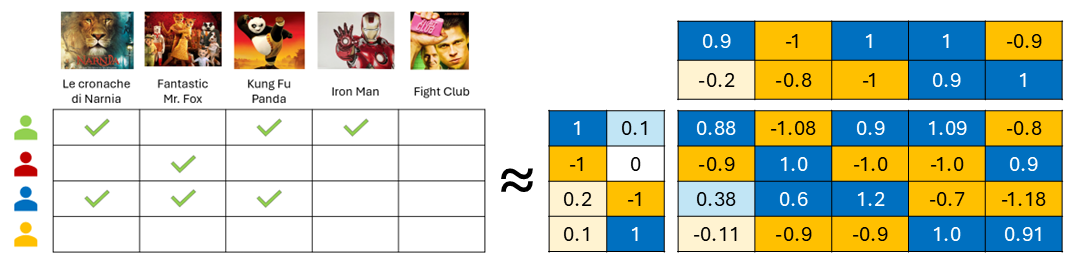
\includegraphics[scale=0.5]{figures/matrix_factorization.PNG}
    \caption{rappresentazione della matrice $R$ come prodotto delle due matrici $W$ e $H$}
    \label{fig:matrix_factorization}
\end{figure}

Questa approssimazione riduce la dimensionalità dei dati, semplifica il modello e cattura le relazioni principali presenti nella matrice originaria.

Un celebre esempio dell'efficacia di questa tecnica nei sistemi di \textit{recommendation} è il \textit{Netflix Prize} del 2006. Il team vincente la utilizzò per migliorare le previsioni di rating del 10\% rispetto al sistema originario di Netflix \cite{TheNP}.

I principali vantaggi nel suo utilizzo sono la scalabilità, poiché i modelli sono efficienti da memorizzare e computare, e la capacità di generalizzazione, in quanto riescono a catturare relazioni latenti non esplicitamente osservate. Tuttavia, esistono anche alcuni limiti, tra cui il problema della \textit{cold start}, che rende difficile raccomandare per nuovi utenti o nuovi item, e la sparsità, che può portare a una una bassa qualità delle raccomandazioni\cite{SVD_analysis}.

Pur con alcune limitazioni, essa costituisce la base per molti degli algoritmi di \textit{recommendation} più efficaci oggi in uso, ed è spesso integrata con approcci più complessi, come i modelli Deep Learning o i grafi.


\section{Tipologie di feedback}

I sistemi di raccomandazione si basano sull’analisi delle preferenze degli utenti, espresse attraverso due principali modalità: feedback esplicito e feedback implicito. Ogni modalità presenta vantaggi, limitazioni e diverse tipologie di approcci.

\subsection{Feedback Esplicito}

Il feedback esplicito si riferisce a tutte quelle situazioni in cui l’utente comunica consapevolmente il proprio grado di interesse per un oggetto. Esempi includono le valutazioni da $1$ a $5$ stelle per i prodotti su \textit{Amazon} o il pollice su/giù per i video su \textit{YouTube} o semplicemente il \textit{like} su \textit{Instagram}.

I modelli che utilizzano feedback espliciti predicono il \textit{rating} che un dato utente assegnerebbe ad un \text{item}. Per esempio predicono che l'utente $u$ darebbe una votazione di $4$ su $5$ per la serie $i$.

Questi dati forniscono un segnale diretto, ma presentano però anche delle limitazioni:

\begin{itemize}
    \item più difficili da ottenere: richiedono che l’utente lasci intenzionalmente il suo riscontro
    \item rari nel mondo reale: molti utenti non lasciano mai valutazioni, dando origine a dati molto sparsi
    \item possono introdurre bias: ad esempio, utenti soddisfatti sono più propensi a lasciare valutazioni rispetto a quelli neutrali o insoddisfatti o viceversa
\end{itemize}

Nonostante ciò, il feedback esplicito rimane una delle fonti più affidabili per l’addestramento di modelli di raccomandazione, in quanto consente di formulare il problema come una regressione delle valutazioni mancanti~\cite{Implicit_feedback}.

\subsection{Feedback Implicito}

Il feedback implicito, al contrario, non è fornito direttamente dall’utente, ma viene dedotto osservando i suoi comportamenti. Esempi tipici includono:

\begin{itemize}
    \item cronologia degli acquisti
    \item cronologia di navigazione
    \item pattern di ricerca
    \item tempo di permanenza su una pagina
    \item interazioni come click, visualizzazioni o movimenti del mouse
    \item acquisto o meno di un prodotto
\end{itemize}

I feedback impliciti possono essere raccolti facilmente in modo automatico e passivo senza che l'utente debba interagire intenzionalmente. Inoltre, sono molto più abbondando rispetto alla controparte esplicita. Forniscono una rappresentazione più completa del comportamento degli utenti, specialmente in contesti in cui il feedback esplicito è assente o insufficiente.

I modelli che utilizzano feedback impliciti non forniscono un \textit{rating} ma uno \textit{score} numerico per la coppia utente-\textit{item}. Questo numero da solo non ha alcun significato, ma messo in relazioni con altri \textit{score}, calcolati per lo stesso utente con \textit{item} diversi, permette di ordinare gli \textit{item} in base alla preferenza predetta dell’utente.

L'utilizzo di dati impliciti può creare complicazioni:

\begin{itemize}
    \item ambiguità: un’azione (es. visualizzazione di un contenuto) non implica necessariamente una preferenza positiva
    \item rumore nei dati: molte interazioni potrebbero essere accidentali o non intenzionali
    \item assenza di segnali negativi chiari: è difficile distinguere tra mancanza di interesse e mancata esposizione all’oggetto
\end{itemize}


\subsection{Approcci ibridi}

Poiché ciascuna forma di feedback fornisce informazioni diverse, un approccio ibrido è spesso preferibile. Ad esempio, nei sistemi che dispongono di valutazioni esplicite, il feedback implicito può essere utilizzato per arricchire il contesto dell’utente, migliorando le prestazioni del modello nei casi in cui i dati espliciti siano scarsi. I modelli basati sul Deep Learning possono essere progettati per combinare diverse fonti, sfruttando il feedback implicito arricchito da attributi contestuali (tempo, luogo, dispositivo, ecc.) per ottimizzare la previsione.
% \chapter{Algoritmi}\label{algoritmi}

\section{Notazione}\label{notazione}

La notazione utilizzata è la seguente:

\begin{itemize}
    \item \textit{user}: l'utente
    \item \textit{item}: l'oggetto
    \item \textit{rating}: valutazione/i
    \item $m$: numero di \textit{user}
    \item $n$: numero di \textit{item}
    \item $R$: l'insieme di tutti i \textit{rating}/interazioni.
    \item $R_{train}$, $R_{test}$ e $\hat{R}$ indicano il set di addestramento, il set di test e l'insieme dei \textit{rating} previsti.
    \item $U$ : l'insieme di tutti gli \textit{user}. $u$ e $v$ indicano gli \textit{user}.
    \item $I$ : l'insieme di tutti gli \textit{item}. $i$ e $j$ indicano gli \textit{item}.
    \item $U_i$ : l'insieme di tutti gli \textit{user} che hanno valutato l'\textit{item} $i$.
    \item $U_{ij}$ : l'insieme di tutti gli \textit{user} che hanno valutato sia l'\textit{item} $i$ che l'\textit{item} $j$.
    \item $I_u$ : l'insieme di tutti gli \textit{item} valutati dallo \textit{user} $u$.
    \item $I_{uv}$ : l'insieme di tutti gli \textit{item} valutati sia dallo \textit{user} $u$ che dallo \textit{user} $v$.
    \item $r_{ui}$ : il \textit{rating} \textit{vero} dello \textit{user} $u$ per l'\textit{item} $i$.
    \item $\hat{r}_{ui}$ : il \textit{rating} \textit{stimato} dello \textit{user} $u$ per l'\textit{item} $i$.
    \item $b_{ui}$ : il \textit{rating} di base dello \textit{user} $u$ per l'\textit{item} $i$.
    \item $\mu$ : la media di tutti i \textit{rating}.
    \item $\mu_u$ : la media di tutti i \textit{rating} dati dallo \textit{user} $u$.
    \item $\mu_i$ : la media di tutti i \textit{rating} date all'\textit{item} $i$.
    \item $\sigma_u$ : la deviazione standard di tutti i \textit{rating} dati dallo \textit{user} $u$.
    \item $\sigma_i$ : la deviazione standard di tutte le valutazioni date all'\textit{item} $i$.
    \item $N_i^k(u)$ : i $k$ vicini più prossimi dello \textit{user} $u$ che hanno valutato l'\textit{item} $i$. Questo insieme è calcolato utilizzando una metrica di similarità.
    \item $N_u^k(i)$ : i $k$ vicini più prossimi dell'\textit{item} $i$ che sono valutati dallo \textit{user} $u$. Questo insieme è calcolato utilizzando una metrica di similarità.
    \item $\gamma$: iperparametro, il \textit{learning rate} utilizzato per l'algoritmo SGD.
    \item $\lambda$: iperparametro, corrisponde al fattore di regolarizzazione nella funzione obbiettivo
    \item $\hat{x}_{uij}$: score che rappresenta la preferenza dello \textit{user} \textit{i} per l'\textit{item} \textit{i} rispetto all'\textit{item} \textit{j}
    \item $N$: numero di epoche per l'algoritmo \textit{Gradient Descent}.
\end{itemize}

\section{Algoritmi per il feedback esplicito}\label{algoritmi-per-feedback-esplicito}

\subsection{Matrix Factorization}

\subsubsection{SVD}\label{svd}

L'algoritmo SVD (\textit{singular value decomposition}), è stato reso popolare da Simon Funk durante la competizione \textit{the Netflix Prize} dimostrando come modelli di fattorizzazione matriciale sono superiori alle tecniche classiche basate su \textit{nearest neighbor}\ref{knn} per
la produzione di raccomandazioni.

I modelli di \textit{matrix factorization} mappano gli \textit{user} e gli \textit{item} in uno spazio latente comune di dimensione $k$, che rappresenta il numero di caratteristiche latenti. Ogni \textit{item} $i$ è associato a un vettore $q_i$ di dimensione $k$, che misura quanto l'\textit{item} possieda ciascuna di queste caratteristiche latenti. Per ogni \textit{user} $u$, invece, il vettore $p_u$ misura l'interesse dello \textit{user} per gli \textit{item}. Il numero di fattori è un iperparametro dell'algoritmo.

In questo spazio, le interazioni tra \textit{user} e \textit{item} vengono modellate come prodotti scalari tra i rispettivi vettori. Lo spazio latente cerca di spiegare i \textit{rating} caratterizzando sia gli \textit{item} che gli textit{user} in base a fattori che vengono automaticamente dedotti. Ad esempio, se gli \textit{item} sono film, i fattori potrebbero appresentare il genere piuttosto che un altro (e.g. Azione contro Drama), profondità della trama o il concetto di "adatto ai bambini".

Il prodotto scalare risultante cattura l'interazione tra lo \textit{user} $u$ e l'\textit{item} $i$, che corrisponde all'interesse complessivo dello \textit{user} per le caratteristiche dell'\textit{item}. Il \textit{rating} finale viene ottenuto aggiungendo anche i predittori di base sopra menzionati, che dipendono solo dallo \textit{user} o dall'\textit{item}. Pertanto, un \textit{rating} viene predetto dalla regola~\cite{SVD_analysis}~\cite{Recommendation_book}:

\[
\hat{r}_{ui} = \mu + b_u + b_i + q_i^T p_u
\]

Dove:
\begin{itemize}
    \item $ b_u $ e $ b_i $ sono i bias dello \textit{user} $u$ e dell'\textit{item} $i$ rispettivamente. Sono una sorta di correzione basata sull'effetto dello \textit{user} e dell'\textit{item}.
    \item $ q_i^T p_u $ è il prodotto interno tra i vettori latenti dello \textit{user} e dell'\textit{item}.
\end{itemize}

Se lo \textit{user} $u$ è sconosciuto, allora il bias $b_u$ e i fattori $p_u$ vengono considerati uguali a zero. Lo stesso vale per
l'\textit{item} $i$, con $b_i$ e $q_i$ anch'essi assunti uguali a zero.

Per apprendere i parametri del modello ($b_u$, $b_i$, $p_u$, $q_i$), si minimizza l'errore quadratico regolarizzato tra le \textit{rating} reali e quelle previste. L'errore quadratico è dato da:

\[
\min \sum\limits_{(u,i) \in K} \left( (r_{ui} - \hat{r}_{ui})^2 + \lambda (\|q_i\|^2 + \|p_u\|^2 + b_u^2 + b_i^2) \right)
\]


Dove il primo termine è l'errore quadratico tra le \textit{rating} previste e reali e il secondo termine è la regolarizzazione, che penalizza valori troppo grandi per i parametri $b_u$, $b_i$, $p_u$, $q_i$ per evitare l'overfitting.

Per ottimizzare questi parametri, viene usata la \textit{Stochastic Gradient Descent} (SGD), che aggiorna i parametri dopo ogni  esempio di training (ad esempio, per ogni \textit{rating} di un \textit{user}).

Per ogni \textit{rating} ($r_{ui}$) data, viene fatta una previsione ($\hat{r}_{ui}$), e l'errore di previsione associato ($e_{ui} = r_{ui} - \hat{r}_{ui}$) viene calcolato. Per un dato caso di addestramento ($r_{ui}$), modifichiamo i parametri spostandoci nella
direzione opposta al gradiente, ottenendo:

\begin{itemize}
    \item $b_u \leftarrow b_u + \gamma \cdot e_{ui}$
    \item $b_i \leftarrow b_i + \gamma \cdot e_{ui}$
    \item $q_i \leftarrow q_i + \gamma \cdot e_{ui} \cdot p_u$
    \item $p_u \leftarrow p_u + \gamma \cdot e_{ui} \cdot q_i$
\end{itemize}

Queste formule vengono utilizzate per aggiornare i parametri durante l'addestramento del modello, in modo da ridurre l'errore tra le
\textit{rating} reali e quelle previste.

Per ottenere un ulteriore miglioramento, si possono applicare $\gamma$ e $\lambda$ separati per i bias degli \textit{user}, i bias degli
\textit{item} e i fattori stessi~\cite{SVD_optimized}.

I punti di forza dell'algoritmo sono:

\begin{itemize}
    \item semplicità: l'algoritmo SVD è relativamente semplice da comprendere e implementare.
    \item riduzione della dimensionalità: l'algoritmo permette di ridurre la dimensione del problema mappando sia gli \textit{user} che gli \textit{item} in uno spazio latente di dimensione inferiore, gestendo la sparsità delle matrici. Funziona molto bene quando la matrice delle valutazioni è abbastanza completa. 
    \item caratteristiche latenti: identifica strutture sottostanti che non sono immediatamente evidenti.
\end{itemize}

L'algoritmo soffre anche di diverse problematiche:

\begin{itemize}
    \item problemi con la sparsità: può produrre raccomandazioni imprecise quando la matrice delle valutazioni è troppo sparsa, perché la decomposizione non riesce a estrarre informazioni significative. 
    \item non tiene conto di informazioni aggiuntive: non considera altri fattori come informazioni temporali, contenuti aggiuntivi sugli \textit{item} o preferenze esplicite/implicite dello \textit{user} che non sono registrati nella matrice.
    \item computazionalmente costosa: la decomposizione di una matrice grande è costosa in termini di tempo e risorse.
    \item overfitting: se non adeguatamente regolarizzato si rischia l'overfitting.
\end{itemize}

\subsubsection{SVD\protect++}

La precisione delle previsioni può essere migliorata considerando anche il feedback implicito, che fornisce un'indicazione aggiuntiva delle preferenze degli \textit{user}. Questo è particolarmente utile per gli \textit{user} che hanno fornito molto più feedback implicito che esplicito. Anche nei casi in cui il feedback implicito indipendente è assente, è possibile catturare un segnale significativo tenendo conto degli \textit{item} che gli \textit{user} hanno valutato, indipendentemente dal valore del \textit{rating}. Ciò ha portato a diversi metodi (\textit{Asymmetric-SVD}, \textit{SVD++}, \textit{SVD\_KNN}, ecc.~\cite{SVD++, SVD_KNN}) che modellano il fattore \textit{user} in base agli \textit{item} valutati. Il metodo \textit{SVD++} ha dimostrato di offrire una precisione superiore rispetto a \textit{SVD}.

Viene aggiunto un secondo set di fattori degli \textit{item}, che collega ogni \textit{item} $i$ a un vettore di fattori $y_i$ di dimensione $k$. Questi nuovi fattori vengono utilizzati per caratterizzare gli \textit{user} in base al set di \textit{item} che hanno valutato. La nuova predizione si calcola come segue:

\[
\hat{r}_{ui} = \mu + b_u + b_i + q_i^T \left(p_u + |I_u|^{\frac{1}{2}} \sum\limits_{j \in I_u} y_j \right)
\]

Ora, un \textit{user} $u$ viene modellato come $p_u + |I_u|^{\frac{1}{2}} \sum\limits_{j \in I_u} y_j$, mentre la parte $\sum\limits_{j \in I_u} y_j$ rappresenta i feedback impliciti. Poiché i vettori $y_j$ sono centrati intorno a zero grazie alla regolarizzazione $|I_u|^{\frac{1}{2}}$, la varianza rispetto all'intervallo di valori osservati $|I_u|$ viene stabilizzata.

I parametri del modello vengono determinati minimizzando la funzione di errore quadratico regolarizzato, utilizzando sempre \textit{stochastic gradient descent}. Si itera su tutti i \textit{rating}:

\begin{itemize}
  \item $b_u \leftarrow b_u + \gamma \cdot (e_{ui} - \lambda \cdot b_u)$
  \item $b_i \leftarrow b_i + \gamma \cdot (e_{ui} - \lambda \cdot b_i)$
  \item $q_i \leftarrow q_i + \gamma \cdot \left( e_{ui} \cdot \left( p_u + |I_u|^{-\frac{1}{2}} \sum\limits_{j \in I_u} y_j \right) - \lambda \cdot q_i \right)$
  \item $p_u \leftarrow p_u + \gamma \cdot (e_{ui} \cdot q_i - \lambda \cdot p_u)$
  \item $\forall j \in I_u: \quad y_j \leftarrow y_j + \gamma \cdot \left( e_{ui} \cdot |I_u|^{-\frac{1}{2}} \cdot q_i - \lambda \cdot y_j \right)$
\end{itemize}

È possibile introdurre diversi tipi di feedback implicito nel modello simultaneamente, utilizzando set aggiuntivi di fattori degli \textit{item}.

I punti di forza dell'algoritmo sono:

\begin{itemize}
    \item miglioramento della personalizzazione: SVD++ è un miglioramento significativo rispetto a SVD, poiché prende in considerazione anche l'influenza degli \textit{item} che lo \textit{user} ha già valutato nel termine $\sum\limits_{j \in I_u} y_j$, il che lo rende molto più sensibile alle preferenze individuali dello \textit{user}.
    \item migliore gestione della sparsità: poiché SVD++ tiene conto dei feedback impliciti, riesce a fare previsioni migliori anche quando la matrice delle valutazioni è sparsa.
    \item previsioni più accurate: i feedback impliciti aiutano a produrre previsioni più accurate, soprattutto in scenari dove gli \textit{user} hanno interagito con più \textit{item}.
\end{itemize}

L'algoritmo soffre anche di diverse problematiche:

\begin{itemize}
    \item complessità computazionale maggiore: la necessità di aggiornare $y_i$ aumenta il carico computazionale.
    \item richiede più dati: poiché prende in considerazione anche i feedback impliciti, ha bisogno di un numero maggiore di dati per generare previsioni precise.
    \item overfitting: SVD++ è più propenso a overfitting su dataset piccoli.
\end{itemize}

\subsubsection{NMF}\label{nmf}

Un algoritmo di \textit{collaborative filtering} basato sulla \textit{fattorizzazione matriciale non negativa}.  

Questo algoritmo è molto simile a SVD\ref{svd} ma con una restrizione che tutti gli elementi devono essere non negativi. Questo ha senso, ad esempio, quando si tratta di rating o quantità (che non possono essere negativi).

L'idea è approssimare la matrice $R$ come prodotto di due matrici più piccole:

\[
R \approx WH
\]

dove:
\begin{itemize}
    \item $W \in \mathbb{R}_{\geq 0}^{m \times k}$ rappresenta la matrice dei profili latenti degli \textit{user};
    \item $H \in \mathbb{R}_{\geq 0}^{k \times n}$ rappresenta la matrice dei profili latenti degli \textit{item};
    \item $k$ è il numero di fattori latenti e iperparametro dell'algoritmo
\end{itemize}

Il \textit{rating} stimato dello \textit{user} $u$ per l'\textit{item} $i$ è calcolato come~\cite{NMF2}~\cite{NMF3}:

\[
\hat{r}_{ui} = \sum_{f=1}^k W_{uf} H_{fi} = q_i^T p_u
\]

dove i fattori \textit{user} e articolo vengono mantenuti positivi

L'obiettivo di apprendimento è minimizzare l'errore quadratico sui \textit{rating} osservati nel set di addestramento $R_{train}$:

\[
\min_{W, H} \sum_{(u,i) \in R_{train}} \left( r_{ui} - \hat{r}_{ui} \right)^2 \quad \text{s.t.} \quad W \geq 0,\ H \geq 0
\]

In forma matriciale, questo si può esprimere come:

\[
\min_{W, H} \ \| R_{train} - WH \|_F^2 \quad \text{con} \quad W \geq 0,\ H \geq 0
\]

dove $\| \cdot \|_F$ è la norma di Frobenius.

La procedura di ottimizzazione è una SGD regolarizzata~\cite{NMF} con una scelta specifica della dimensione del passo che garantisce la non negatività dei fattori, a condizione che anche i loro valori iniziali siano positivi.

A ogni iterazione i fattori vengono aggiornati come segue:

\begin{equation}
    \begin{split}
        p_{uf} &\leftarrow p_{uf} \cdot \frac{\sum\limits_{i \in I_u} q_{if} \cdot r_{ui}}{\sum\limits_{i \in I_u} q_{if} \cdot \hat{r}_{ui} + \lambda_u |I_u| p_{uf}}\\
        q_{if} &\leftarrow q_{if} \cdot \frac{\sum\limits_{u \in U_i} p_{uf} \cdot r_{ui}}{\sum\limits_{u \in U_i} p_{uf} \cdot \hat{r}_{ui} + \lambda_i |U_i| q_{if}}
    \end{split}
\end{equation}

Questo algoritmo è altamente dipendente dai valori iniziali con cui vengono inizializzate le matrici $H$ e $W$. I fattori latenti degli \textit{user} e degli \textit{item} vengono inizializzati casualmente in modo uniforme tra un minimo e un massimo, solitamente nell'intervallo $[0, 1]$.

Gli iper-parametri $\lambda_u$ e $\lambda_i$ corrispondono alla regolarizzazione rispettivamente per \textit{user} e \textit{item}.

Anche in questo caso si può utilizzare la predizione con l'utilizzo di baseline\ref{svd}.

\[
\hat{r}_{ui} = \mu + b_u + b_i + q_i^T p_u
\]

garantendo comunque fattori positivi. Le baselines sono ottimizzate nello stesso modo dell'algoritmo SVD. Pur producendo una migliore accuratezza, la versione che utilizza baseline sembra molto incline all'overfitting, che può essere ridotto diminuendo $k$ o aumentando la regolarizzazione.

NFM, grazie al vincolo della non negatività, è più interpretabile di SVD: i valori nelle matrici fattorizzate $W$ e $H$ sono tutti $\geq 0$, quindi possono essere interpretati come pesi o intensità (es. quanto uno \textit{user} apprezza un certo genere, quanto un \textit{item} rappresenta un tema).

L'algoritmo soffre anche di diverse problematiche:

\begin{itemize}
    \item dipendenza dall'inizializzazione: l'algoritmo può convergere a minimi locali diversi a seconda dei valori iniziali, e non garantisce una soluzione unica o ottima
    
    \item non adatta per dati con valori negativi: NMF non può gestire valori negativi nei dati di input, a differenza di SVD
    
    \item convergenza più lenta: rispetto ad altri metodi la convergenza può essere più lenta e richiede tuning di più parametri
    \item mancanza di soluzione chiusa: SVD può gestire valori negativi e ha una soluzione ottima in termini di errore quadratico minimo
\end{itemize}

\subsection{KNN (K-Nearest Neighbors)}\label{knn}
Si tratta di algoritmi derivati direttamente da un approccio di base basato sui \textit{nearest neighbors}.

Gli algoritmi ispirati al KNN (\textit{K Nearest Neighbors}) sono una classe di algoritmi di raccomandazione che si basano sull'idea che gli \textit{user} simili tendono a valutare gli stessi \textit{item} in modo simile. Questi algoritmi sono semplici da implementare e possono essere molto efficaci per problemi di raccomandazione a piccola scala.

Il numero effettivo di vicini che vengono considerati per calcolare la predizione è minore o uguale a $k$: potrebbero non esserci abbastanza vicini e/o gli insiemi $N_i^k(u)$ e $N_u^k(i)$ includono solo vicini per i quali la misura di similarità è positiva (non avrebbe senso considerare \textit{user} o \textit{item} correlati negativamente).

$k$ è un iperparametro di ciascun algoritmo.

Alcune misure di similarità, sia per \textit{user} che per \textit{item}, sono:
\begin{itemize}
    \item Coseno:
        \[
        \text{cosine sim}(u, v) = \frac{\sum\limits_{i \in I_{uv}} r_{ui} \cdot r_{vi}}{\sqrt{\sum\limits_{i \in I_{uv}} r_{ui}^2} \cdot \sqrt{\sum\limits_{i \in I_{uv}} r_{vi}^2}}
        \]
        oppure
        \[
        \text{cosine sim}(i, j) = \frac{\sum\limits_{u \in U_{ij}} r_{ui} \cdot r_{uj}}{\sqrt{\sum\limits_{u \in U_{ij}} r_{ui}^2} \cdot \sqrt{\sum\limits_{u \in U_{ij}} r_{uj}^2}}
        \]
    \item \textit{Mean Square Difference} (MSD):
        \[
        \text{msd}(u, v) = \frac{1}{|I_{uv}|} \cdot \sum\limits_{i \in I_{uv}} (r_{ui} - r_{vi})^2
        \]
        oppure
        \[
        \text{msd}(i, j) = \frac{1}{|U_{ij}|} \cdot \sum\limits_{u \in U_{ij}} (r_{ui} - r_{uj})^2
        \]
        La similarità è calcolata come:
        \begin{align*}
            \text{msd sim}(u, v) &= \frac{1}{\text{msd}(u, v) + 1} \\
            \text{msd sim}(i, j) &= \frac{1}{\text{msd}(i, j) + 1}
        \end{align*}
        Il termine $+1$ viene aggiunto per evitare divisioni per zero.
    \item Pearson: Il coefficiente di correlazione di Pearson può essere visto come una similarità del coseno centrato sulla media. Se non ci sono \textit{item} comuni, la similarità è 0 (non -1).
        \[
        \text{pearson sim}(u, v) = \frac{\sum\limits_{i \in I_{uv}} (r_{ui} - \mu_u) \cdot (r_{vi} - \mu_v)}{\sqrt{\sum\limits_{i \in I_{uv}} (r_{ui} - \mu_u)^2} \cdot \sqrt{\sum\limits_{i \in I_{uv}} (r_{vi} - \mu_v)^2}}
        \]
        oppure
        \[
        \text{pearson sim}(i, j) = \frac{\sum\limits_{u \in U_{ij}} (r_{ui} - \mu_i) \cdot (r_{uj} - \mu_j)}{\sqrt{\sum\limits_{u \in U_{ij}} (r_{ui} - \mu_i)^2} \cdot \sqrt{\sum\limits_{u \in U_{ij}} (r_{uj} - \mu_j)^2}}
        \]
    \item Pearson con baseline \cite{Recommendation_book}: calcola il coefficiente di correlazione di Pearson (ridotto) tra tutte le coppie di \textit{user} (o \textit{item}) utilizzando le baseline anziché le medie. Il parametro di riduzione aiuta a evitare l'overfitting quando sono disponibili solo poche valutazioni. Se non ci sono \textit{item} comuni, la similarità è 0 (non -1). Introduce un nuovo iperparametro che corrisponde alla riduzione (o \textit{``shrinkage''}). Se impostato uguale a 0, non viene applicata nessuna riduzione.
        \[
        \text{pearson baseline sim}(u, v) = \hat{\rho}_{uv} = \frac{\sum\limits_{i \in I_{uv}} (r_{ui} - b_{ui}) \cdot (r_{vi} - b_{vi})}{\sqrt{\sum\limits_{i \in I_{uv}} (r_{ui} - b_{ui})^2} \cdot \sqrt{\sum\limits_{i \in I_{uv}} (r_{vi} - b_{vi})^2}}
        \]
        oppure
        \[
        \text{pearson baseline sim}(i, j) = \hat{\rho}_{ij} = \frac{\sum\limits_{u \in U_{ij}} (r_{ui} - b_{ui}) \cdot (r_{uj} - b_{uj})}{\sqrt{\sum\limits_{u \in U_{ij}} (r_{ui} - b_{ui})^2} \cdot \sqrt{\sum\limits_{u \in U_{ij}} (r_{uj} - b_{uj})^2}}
        \]
        Il coefficiente ridotto si calcola come:
        \begin{align*}
            \text{pearson baseline shrunk sim}(u, v) &= \frac{|I_{uv}| - 1}{|I_{uv}| - 1 + \text{shrinkage}} \cdot \hat{\rho}_{uv} \\
            \text{pearson baseline shrunk sim}(i, j) &= \frac{|U_{ij}| - 1}{|U_{ij}| - 1 + \text{shrinkage}} \cdot \hat{\rho}_{ij}
        \end{align*}
        Per il calcolo della baseline, si consideri la parte di \ref{knn_baseline}.
\end{itemize}

Altro iperparametro da considerare è il supporto minimo, che corrisponde al numero minimo di \textit{item} in comune o il numero minimo di \textit{user} in comune affinché la similarità non sia zero, i.e., se $|I_{uv}| < \text{min support}$, allora $\text{sim}(u, v) = 0$. Lo stesso vale per gli \textit{item}.

\subsubsection{KNN base}

L'algoritmo KNN base è l'algoritmo più semplice. Prevede il  \textit{rating} di un \textit{user} $u$ per un \textit{item} $i$ come la media ponderata dei \textit{rating} degli $k$ vicini più simili di $u$ o $i$, a seconda che si utilizzi un approccio basato sugli \textit{user} o sugli \textit{item}.

La predizione viene calcolata come:

\[
\hat{r}_{ui} = \frac{\sum\limits_{v \in N^k_i(u)} \text{sim}(u, v) \cdot r_{vi}}{\sum\limits_{v \in N^k_i(u)} \text{sim}(u, v)}
\]

oppure

\[
\hat{r}_{ui} = \frac{\sum\limits_{j \in N^k_u(i)} \text{sim}(i, j) \cdot r_{uj}}{\sum\limits_{j \in N^k_u(i)} \text{sim}(i, j)}
\]

dipendentemente dall'approccio utilizzato.

\subsubsection{KNN con la media}
\label{algoritmo-knn-con-la-media}

L'algoritmo è una variante dell'algoritmo KNN base che tiene conto della media dei \textit{rating} degli \textit{user} o degli \textit{item}.

La predizione viene calcolata come:

\[
\hat{r}_{ui} = \mu_u + \frac{\sum\limits_{v \in N_k(u)} \text{sim}(u, v) \cdot (r_{vi} - \mu_v)}{\sum\limits_{v \in N_k(u)} \text{sim}(u, v)}
\]

oppure

\[
\hat{r}_{ui} = \mu_i + \frac{\sum\limits_{j \in N^k_u(i)} \text{sim}(i, j) \cdot (r_{uj} - \mu_j)}{\sum\limits_{j \in N^k_u(i)} \text{sim}(i, j)}
\]

dipendentemente dall'approccio utilizzato.

\subsubsection{KNN normalizzato}
\label{algoritmo-knn-normalizzato}

L'algoritmo è una variante dell'algoritmo che utilizza la media con l'aggiunta della normalizzazione \textit{z-score}, con la deviazione standard dello \textit{user} o dell'\textit{item}, dei \textit{rating} corrispondenti prima di calcolare la similarità.

La predizione viene calcolata come:

\[
\hat{r}_{ui} = \mu_u + \sigma_u \frac{\sum\limits_{v \in N^k_i(u)} \text{sim}(u, v) \cdot (r_{vi} - \mu_v) / \sigma_v}{\sum\limits_{v \in N^k_i(u)} \text{sim}(u, v)}
\]

oppure

\[
\hat{r}_{ui} = \mu_i + \sigma_i \frac{\sum\limits_{j \in N^k_u(i)} \text{sim}(i, j) \cdot (r_{uj} - \mu_j) / \sigma_j}{\sum\limits_{j \in N^k_u(i)} \text{sim}(i, j)}
\]

dipendentemente dall'approccio utilizzato.

\subsubsection{KNN con baseline}\label{knn_baseline}
\label{knn-con-baseline}

L'algoritmo KNN con baseline \cite{KNN_baseline} è una variante dell'algoritmo base che tiene conto degli effetti di bias degli \textit{user} o degli \textit{item}.

La predizione viene calcolata come:

\[
\hat{r}_{ui} = b_{ui} + \frac{\sum\limits_{v \in N^k_i(u)} \text{sim}(u, v) \cdot (r_{vi} - b_{vi})}{\sum\limits_{v \in N^k_i(u)} \text{sim}(u, v)}
\]

oppure

\[
\hat{r}_{ui} = b_{ui} + \frac{\sum\limits_{j \in N^k_u(i)} \text{sim}(i, j) \cdot (r_{uj} - b_{uj})}{\sum\limits_{j \in N^k_u(i)} \text{sim}(i, j)}
\]

dipendentemente dall'approccio utilizzato.

La baseline $b_{ui}$ viene calcolata come:

\[
b_{ui} = \mu + b_u + b_i
\]

Per calcolare $b_u$ e $b_i$, occorre minimizzare il seguente errore quadratico regolarizzato:

\[
\sum\limits_{r_{ui} \in R_{train}} \left(r_{ui} - \mu + b_u + b_i\right)^2 + \lambda \left(b_u^2 + b_i^2 \right).
\]

Il termine di regolarizzazione $\lambda \left(b_u^2 + b_i^2 \right)$ serve per evitare l'overfitting penalizzando la grandezza dei parametri.

La minimizzazione può essere effettuata tramite \textit{Stochastic Gradient Descent} o \textit{Alternating Least Squares}.

Per \textit{Alternating Least Squares}, i due valori di $b_u$ e $b_i$ si ottengono come:

\[
b_i = \frac{\sum\limits_{r_{ui} \in R_{train}} (r_{ui} - \mu)}{\lambda_2 + |U_i|}
\]

e

\[
b_u = \frac{\sum\limits_{r_{ui} \in R_{train}} (r_{ui} - \mu - b_i)}{\lambda_3 + |I_u|}
\]

I punti di forza della famiglia di algoritmi KNN sono:
\begin{itemize}
    \item semplicità: Gli algoritmi KNN sono facili da capire e implementare. L'idea di base di trovare ``vicini'' simili è intuitiva e facilmente comprensibile.
    \item nessuna assunzione sui dati: l'algoritmo non fa assunzioni sulla distribuzione dei dati. Questo lo rende flessibile e adatto a una varietà di dataset.
    \item aggiornamento: l'aggiunta di nuovi dati non richiede una fase di addestramento esplicita. Questo lo rende utile in ambienti in cui i dati cambiano frequentemente o per previsioni online.
    \item flessibilità: KNN può essere utilizzato sia per problemi di raccomandazione basati su \textit{user} che basati su \textit{item}.
\end{itemize}

Gli algoritmi soffrono anche di diverse problematiche:
\begin{itemize}
    \item costo computazionale: KNN può essere computazionalmente costoso, soprattutto con set di dati di grandi dimensioni.
    \item requisiti di memoria: KNN richiede la memorizzazione dell'intero set di dati, il che può essere problematico per set di dati molto grandi.
    \item sensibilità alla scelta di $k$: La scelta del valore di k può avere un impatto significativo sulle prestazioni di KNN. Un valore di k troppo piccolo può portare a un overfitting, mentre un valore di k troppo grande può portare a un underfitting. Inoltre, la ricerca dei $k$ vicini più prossimi richiede il calcolo delle distanze tra tutti i punti dati.
    \item gestione della sparsità dei dati: la sparsità può rendere difficile trovare vicini significativi e quindi portare a raccomandazioni di bassa qualità.
\end{itemize}

\subsection{CoClustering}\label{coclustering}

La soluzione proposta da Thomas George e Srujana Merugu~\cite{Co-Clustering} utilizza il \textit{co-clustering}. Questa tecnica viene utilizzata per raggruppare simultaneamente due entità in un dataset. Nel caso di un sistema di \textit{recommendation} basato su \textit{collaborative filtering}, l'obiettivo è trovare gruppi di \textit{user} simili e gruppi di \textit{item} simili. Il co-clustering cerca di partizionare simultaneamente le righe (\textit{user}) e le colonne (\textit{item}) della matrice dei \textit{rating} in modo tale che gli \textit{user} all'interno dello stesso co-cluster abbiano comportamenti di valutazione simili e \textit{item} all'interno dello stesso co-cluster siano valutati in modo simile dagli \textit{user} del co-cluster. Il numero di cluster è da definire a priori sia per gli \textit{user} che per gli \textit{item}. Il processo di co-clustering è simile al clustering tradizionale, ma mentre nel clustering classico si raggruppa solo per righe o colonne, nel co-clustering si raggruppano contemporaneamente. 

L'algoritmo, nella fase di inizializzazione, assegna casualmente i co-cluster a \textit{user} e \textit{item}. Durante l'esecuzione i co-cluster vengono aggiornati iterativamente, per cercare di migliorare la qualità del raggruppamento, alternando tra il raggruppamento degli \textit{user} e degli \textit{item} fino a convergenza. Una volta che i co-cluster sono definiti si può calcolare la media dei \textit{rating} all'interno di ciascun co-cluster. $ \overline{C_{ui}} $ rappresenta la media dei \textit{rating} all'interno del co-cluster che contiene lo \textit{user} $ u $ e l'\textit{item} $ i $. In altre parole, è il \textit{rating} medio tra gli \textit{user} e gli \textit{item} che appartengono allo stesso co-cluster.

Si può quindi definire la predizione come

\[
\hat{r}_{ui} = \overline{C_{ui}} + (\mu_u - \overline{C_u}) + (\mu_i - \overline{C_i})
\]

dove $\overline{C_u}$ è la media dei \textit{rating} del cluster di $u$ e $\overline{C_i}$ è la media dei \textit{rating} del cluster di $i$. $ \mu_u - \overline{C_u} $ e $ \mu_i - \overline{C_i} $ vengono definiti \textit{bias}. Se: 
\begin{itemize}
  \item \textit{user} mancante: la previsione è $ \overline{C_i} $
  \item \textit{item} mancante: la previsione è $ \overline{C_u} $
  \item se sia \textit{user} che \textit{item} sono mancanti: la previsione è $ \mu $, la media generale dei rating.
\end{itemize}

I punti di forza dell'algoritmo sono:

\begin{itemize}
  \item Scalabilità: l'algoritmo di co-clustering può essere facilmente parallelizzato, il che lo rende adatto per sistemi di \textit{recommendation} con grandi quantità di dati.
  \item Gestione dei comportamenti complessi: la previsione tiene conto sia del co-cluster, che considera simultaneamente i raggruppamenti di \textit{user} e \textit{item}, sia dei cluster singoli per \textit{user} e \textit{item}. Questo permette di considerare diversità e similarità sia individualmente che insieme, migliorando le previsioni.
  \item Gestione semplice degli aggiornamenti: quando nuovi dati sono aggiunti al sistema, è possibile aggiornare solo i co-cluster rilevanti senza dover ricalcolare tutto da zero. Questo è particolarmente utile per scenari dinamici e sistemi in tempo reale.
  \item Gestione della sparsità: poiché l'algoritmo raggruppa \textit{user} e \textit{item} simili, riduce l'effetto della sparsità permettendo di migliorare la qualità delle previsioni anche quando i dati disponibili sono pochi o incompleti.
\end{itemize}

L'algoritmo soffre anche di diverse problematiche:

\begin{itemize}
  \item Sensibilità ai co-cluster: la qualità delle previsioni dipende molto dal numero di co-cluster scelto e dalla loro qualità. Se il numero di co-cluster è troppo basso, il modello potrebbe non riuscire a catturare le complessità dei dati e fare previsioni imprecise. Se il numero è troppo alto, il modello potrebbe overfittare i dati di addestramento, riducendo la sua generalizzazione. Inoltre, se i co-cluster non sono ben definiti, il modello potrebbe produrre previsioni inaccurate. La scelta iniziale dei co-cluster è fondamentale. Una soluzione è quella di utilizzare l'algoritmo \textit{K-means} per definire la posizione iniziale dei cluster.
  \item Bias del co-cluster: $ \mu_u - \overline{C_u} $ e $ \mu_i - \overline{C_i} $ potrebbero non essere sempre utili in tutte le situazioni. Alcuni \textit{user} o \textit{item} potrebbero avere comportamenti che non sono ben rappresentati dai co-cluster e il modello potrebbe non adattarsi bene a queste situazioni. Ad esempio, \textit{user} che tendono a esprimere \textit{rating} bassi potrebbero non essere gestiti correttamente.
  \item Alto costo computazionale iniziale: l'algoritmo ha un alto costo computazionale durante la fase di addestramento, soprattutto con set di dati molto grandi. Anche se è scalabile, l'ottimizzazione del processo di clustering e la ricerca del numero ottimale di co-cluster richiedono parecchia computazione.
  \item Difficoltà di interpretazione: il co-clustering fornisce gruppi di \textit{user} e \textit{item} che potrebbero non essere sempre facili da interpretare o da analizzare in modo intuitivo.
\end{itemize}

Il costo computazionale per l'addestramento è $ O(W^{\text{glob}} + mkl + nkl) $ dove $ W^{\text{glob}} $ corrisponde al numero di valori diversi da 0 nella matrice in input , $l$ corrisponde al numero di cluster per gli \textit{user} e $k$ corrisponde al numero di cluster per gli \textit{item}.

Per il calcolo della predizione, il costo è $O(1)$, in quanto si tratta di operazioni media e il calcolo dei bias.

Per l'aggiornamento quando un nuovo \textit{rating} viene aggiunto o un nuovo \textit{user}/\textit{item} entra nel sistema, l'algoritmo non ricalcola tutto da zero. Invece, utilizza un aggiornamento incrementale parziale, che si basa sull'aggiornamento delle medie delle matrici:

\begin{itemize}
  \item Se il nuovo \textit{rating} riguarda un \textit{user} e un \textit{item} esistenti si aggiornano direttamente le medie.
  \item Se l'\textit{user} o l'\textit{item} è nuovo, viene assegnato temporaneamente a un co-cluster globale di transizione. Le medie vengono aggiornate e, durante la successiva esecuzione dell'algoritmo, il nuovo \textit{user}/\textit{item} viene riassegnato ai co-cluster regolari.
\end{itemize}

L'aggiornamento ha quindi costo pari a $O(1)$.

\subsection{Slope One}\label{slopeone}

L'algoritmo Slope One, introdotto da Daniel Lemire e Anna Maclachlan~\cite{SlopeOne}, è una delle soluzioni più semplici ed efficienti di collaborative filtering.
%
Le caratteristiche che lo rendono un ottimo algoritmo per la \textit{recommendation} sono:
\begin{itemize}
    \item la semplicità e facilità di implementazione
    \item velocità di calcolo: come verrà presentato più avanti alcuni valori calcolati possono essere salvati e aggiornati all'occorrenza rendendo il calcolo molto più veloce
    \item scalabilità: l'algoritmo può essere abbastanza efficace su dataset di dimensioni moderate, soprattutto se si utilizzano tecniche di compressione dei dati
    \item facilità di interpretazione
\end{itemize}
%
Viene proposto un predittore basato su differenze di \textit{rating} lineari che ha un'efficienza $O(nm)$ per predizione e $O(mn^2)$ per addestramento.

L'algoritmo si basa sulla differenza media tra le valutazioni di due \textit{item} per predire il \textit{rating} mancante. La differenza media dei \textit{rating} di due \textit{item} $i$ e $j$ viene calcolata come:

\[
    \text{dev}(i, j) = \frac{1}{|U_{i,j}|} \sum\limits_{u \in U_{i,j}} (r_{u,i} - r_{u,j})
\]

La matrice simmetrica definita da $\text{dev}(i, j)$ può essere computata una volta e aggiornata velocemente quando vengono aggiunti nuovi dati.

La predizione viene dunque calcolata come:

\[
    \hat{r}_{ui} = \mu_u + \frac{1}{|R_i(u)|} \sum\limits_{j \in R_i(u)} \text{dev}(i, j)
\]

dove:

\begin{itemize}
    \item $R_j = \{ i \mid i \in S(u), i \neq j, |S_{j,i}(\chi)| > 0 \}$ è l'insieme degli \textit{item} rilevanti
    \item $S(u)$ è il sottoinsieme degli \textit{item} valutati dallo \textit{user} $u$
    \item $S_{j,i}(\chi)$ è l'insieme di tutte le valutazioni $u$ nel dataset $\chi$ che contengono gli \textit{item} $i$ e $j$
\end{itemize}

\begin{figure}[H]
    \centering
    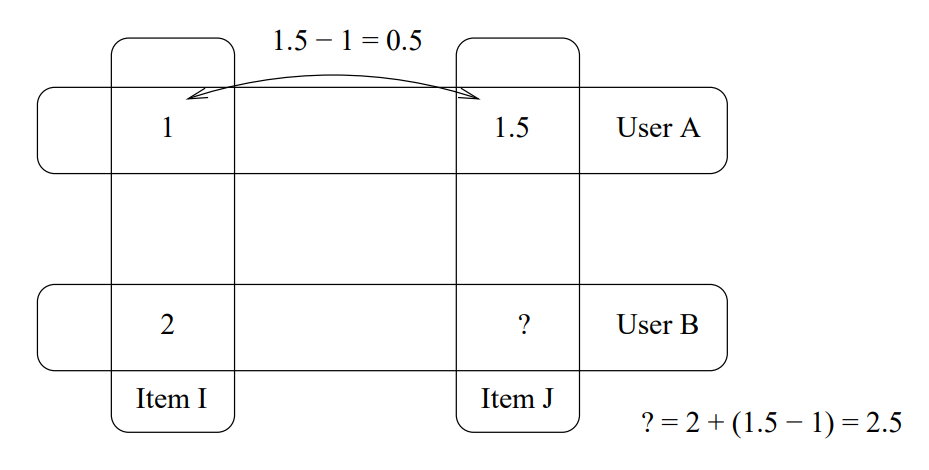
\includegraphics[keepaspectratio]{figures/algorithms/slope_one.PNG}
    \caption{Base dello schema Slope One: le valutazioni dello \textit{user} A di due \textit{item} e la valutazione  dello \textit{user} B di un \textit{item} comune vengono utilizzate per prevedere la valutazione sconosciuta dello \textit{user}.}
    \label{fig:slopeone}
\end{figure}

L'algoritmo soffre anche di diverse problematiche:
\begin{itemize}
    \item sparsità dei dati: le formule presentate prima sono approssimate considerando un dataset non sparso. Nel caso di matrici molto sparse l'algoritmo non sarà in grado di fare previsioni accurate
    \item scalabilità limitata su dataset molto grandi: la memoria necessaria per memorizzare le differenze medie dei \textit{rating} può aumentare rapidamente
    \item non tiene conto nè di personalizzazioni per \textit{user} 
    \item difficoltà a gestire grandi variazioni nelle valutazioni degli utenti
\end{itemize}

L'approccio può essere esteso a modelli ponderati e versioni più avanzate, come per esempio \textit{Weighted Slope One}, che pesa le differenze di \textit{rating} in base alla frequenza di coppie di \textit{item} valutati, e \textit{Regression-based Slope One}, che introduce funzioni non lineari per migliorare la precisione delle previsioni.

\subsection{Evaluation esplicita}\label{evaluation-esplicita}

\section{Algoritmi per il feedback implicito}\label{algoritmi-per-feedback-implicito}

\subsection{ALS (Alternating Least Squares)}\label{als}

Il lavoro di Hu, Koren e Volinsky~\cite{ALS} propone una formulazione adatta a modellare feedback impliciti, come click, acquisti o visualizzazioni.

Si basa sulla \textit{Matrix Factorization}, e una delle sue tecniche di ottimizzazione più efficaci è \textit{ALS (Alternating Least Squares)}, in particolare per dataset con \textit{feedback impliciti}.

L'obiettivo è approssimare la matrice osservata $R \in \mathbb{R}^{m \times n}$ (dove $m$ è il numero di \textit{user} e $n$ il numero di \textit{item}) come il prodotto di due matrici a bassa dimensionalità:

\[
R \approx W H^\top
\]

dove:

\begin{itemize}
    \item $W \in \mathbb{R}^{m \times k}$: matrice dei fattori latenti degli utenti,
    \item $H \in \mathbb{R}^{n \times k}$: matrice dei fattori latenti degli item,
    \item $k$: numero di fattori latenti (dimensione dello spazio latente) e iperparametro.
\end{itemize}

Si definisce la variabile binaria \textit{preferenza} $p_{ui}$ che indica la preferenza per uno \textit{user} \textit{u} per un \textit{item} \textit{i}:
\[
p_{ui} =
\begin{cases}
    1 & \text{se lo \textit{user} } u \text{ ha interagito con l'\textit{item} } i \\
    0 & \text{altrimenti}
\end{cases}
\]

e la confidenza
    
\[
c_{ui} = 1 + \alpha \cdot r_{ui}
\]
dove $r_{ui}$ in questo caso è l'interazione (es. \% visualizzazione o numero di acquisti), e $\alpha$ è un iperparametro che modula l'importanza delle osservazioni positive.

Il problema di ottimizzazione da risolvere è:

\[
\min_{W, H} \sum_{u=1}^m \sum_{i=1}^n c_{ui} (p_{ui} - w_u^\top h_i)^2 + \lambda \left( \sum_u \|w_u\|^2 + \sum_i \|h_i\|^2 \right)
\]

dove:

\begin{itemize}
    \item $w_u$: vettore dei fattori latenti per lo \textit{user} $u$,
    \item $h_i$: vettore dei fattori latenti per l' \textit{item} $i$,
\end{itemize}

Il primo termine rappresenta l'\textit{errore quadratico pesato} tra la preferenza osservata e la previsione del modello. Il secondo termine è una \textit{regolarizzazione} di tipo L2 per evitare overfitting.

Il problema in $(W,H)$ non è convesso (cioè potrebbe avere più minimi locali e non è facile trovare il minimo assoluto) ma lo diventa se si fissa una delle due variabili. Questo significa che si può trovare il minimo facilmente rispetto a $W$ tenendo $H$ fisso e viceversa. Per questo motivo, si usa un metodo iterativo finché non si arriva a una soluzione stabile:

\begin{enumerate}
    \item Si fissa $H$ e si ottimizza $W$,
    \item Si fissa $W$ e si ottimizza $H$,
    \item Si ripete per un numero prefissato di iterazioni $T$.
\end{enumerate}

Fissata $H$, per ogni \textit{user} $u$ si risolve il sistema:

\[
w_u = \left( H^\top C^u H + \lambda I \right)^{-1} H^\top C^u p^u
\]

Analogamente, per ogni \textit{item} $i$:

\[
h_i = \left( W^\top C^i W + \lambda I \right)^{-1} W^\top C^i p^i
\]

dove:

\begin{itemize}
    \item $C^u = \text{diag}(c_{u1}, \dots, c_{un})$,
    \item $p^u = (p_{u1}, \dots, p_{un})^\top$.
\end{itemize}

Il calcolo diretto dell'inversa richiede $\mathcal{O}(k^3)$ per ogni \textit{user}/\textit{item}, troppo oneroso per grandi dataset. Si può invece risolvere il sistema lineare associato:

\[
A x = b \quad \text{con} \quad A = H^\top C^u H + \lambda I, \quad b = H^\top C^u p^u
\]

utilizzando il \textit{metodo del gradiente coniugato (CG)}~\cite{ALS_opt}. Questo metodo è iterativo e richiede solo moltiplicazioni matrice-vettore, con complessità per iterazione $\mathcal{O}(k^2)$.

\begin{algorithm}[H]
    \caption{Metodo del Gradiente Coniugato per risolvere $Ax = b$}
    \begin{algorithmic}[1]
    \Require Matrice $A \in \mathbb{R}^{n \times n}$ simmetrica e definita positiva, vettore $b \in \mathbb{R}^n$, iniziale $x_0$, tolleranza $\epsilon$
    \State $r_0 \gets b - A x_0$
    \State $p_0 \gets r_0$
    \State $k \gets 0$
    \While{$\|r_k\| > \epsilon$ e $k < \text{max\_iter}$}
        \State $\alpha_k \gets \dfrac{r_k^\top r_k}{p_k^\top A p_k}$
        \State $x_{k+1} \gets x_k + \alpha_k p_k$
        \State $r_{k+1} \gets r_k - \alpha_k A p_k$
        \If{$\|r_{k+1}\| < \epsilon$}
            \State \textbf{break}
        \EndIf
        \State $\beta_k \gets \dfrac{r_{k+1}^\top r_{r+1}}{r_k^\top r_k}$
        \State $p_{k+1} \gets r_{k+1} + \beta_k p_k$
        \State $k \gets k + 1$
    \EndWhile
    \State \Return $x_{k+1}$
    \end{algorithmic}
\end{algorithm}
    
Il numero di iterazioni di \textit{GC} è un iperparametro.

Infine, lo score viene calcolato come

\[
\hat{x}_{ui} = w_u^T h_i
\]

I punti di forza dell'algoritmo sono:
\begin{itemize}
    \item efficienza computazionale: il metodo del gradiente coniugato riduce il costo computazionale rispetto all'inversione esplicita delle matrici.
    \item scalabilità: permette di gestire dataset di grandi dimensioni, grazie alla natura iterativa e alla possibilità di eseguire il calcolo in parallelo.
    \item minore uso di memoria rispetto all'inversione diretta: non è necessario costruire esplicitamente la matrice intera da invertire.
    \item velocità di convergenza: in molti casi, bastano poche iterazioni per ottenere una buona approssimazione della soluzione.
    \item supporto gpu: il calcolo iterativo si adatta bene all'accelerazione hardware, migliorando ulteriormente i tempi di addestramento.
\end{itemize}

L'algoritmo soffre anche di diverse problematiche:

\begin{itemize}
    \item approssimazione: il metodo \textit{GC} fornisce una soluzione approssimata, la cui precisione dipende dal numero di iterazioni utilizzate.
    \item sensibilità ai parametri: il numero di iterazioni (\textit{GC steps}) è un iperparametro che va scelto con attenzione per bilanciare accuratezza e prestazioni.
    \item stabilità numerica: se la matrice del sistema è mal condizionata, la convergenza del metodo \textit{GC} può essere lenta o instabile.
    \item maggiore complessità implementativa: integrare \textit{GC} richiede strutture dati e operazioni più sofisticate rispetto all'inversione diretta.
    \item overhead per piccoli dataset: su dataset piccoli, l'uso di \textit{GC} può risultare meno vantaggioso rispetto ad una soluzione esatta diretta.
\end{itemize}

\subsection{BPR (Bayesian Personalized Ranking)}\label{bpr}

Nei sistemi basati su \textit{feedback impliciti}, la mancanza di interazione tra un \textit{user} e un \textit{item} non implica necessariamente una preferenza negativa. Per affrontare tale ambiguità, BPR~\cite{BPR} adotta le seguenti ipotesi:

\begin{itemize}
    \item Se $(u, i) \in R$, cioè lo \textit{user} $u$ ha interagito con l'\textit{item} $i$, allora $u$ preferisce $i$ a tutti gli \textit{item} $j$ con cui non ha interagito.
    \item A partire da questo principio, si costruisce un insieme di triple:
    \[
    D_S := \{(u, i, j) \mid i \in I_u \wedge j \in I \setminus I_u\}
    \]
    dove ogni tripla rappresenta la preferenza dello \textit{user} $u$ per l'\textit{item} $i$ rispetto all'\textit{item} $j$.
\end{itemize}

L'obiettivo di BPR è massimizzare la probabilità a posteriori dei parametri del modello $\Theta$, dati i dati osservati:
\[
\text{BPR-Opt} = \sum_{(u, i, j) \in D_S} \ln \sigma(\hat{x}_{uij}) - \lambda_\Theta ||\Theta||^2
\]
dove:
\begin{itemize}
    \item $\hat{x}_{uij} = \hat{x}_{ui} - \hat{x}_{uj}$ è la differenza tra le valutazioni stimate per $i$ e $j$;
    \item $\sigma(x) = \frac{1}{1 + e^{-x}}$ è la funzione sigmoide;
    \item $\lambda_\Theta$ è il parametro di regolarizzazione.
\end{itemize}

Questo criterio è strettamente legato all'ottimizzazione dell'AUC (Area Under the ROC Curve), che misura la qualità del ranking.

Per prima cosa si calcola il gradiente di BPR-Opt come:

\[
\frac{\partial \text{BPR-Opt}}{\partial \Theta} =
\sum_{(u,i,j) \in D_S} 
\frac{\partial}{\partial \Theta} \ln \sigma(\hat{x}_{uij}) - 
\lambda \frac{\partial}{\partial \Theta} ||\Theta||^2
\]

\[
\propto 
\sum_{(u,i,j) \in D_S} 
\frac{-e^{-\hat{x}_{uij}}}{1 + e^{-\hat{x}_{uij}}} 
\cdot \frac{\partial}{\partial \Theta} \hat{x}_{uij} 
- \lambda \Theta
\]

L'ottimizzazione di BPR-Opt viene effettuata tramite \textit{stochastic gradient descent}. I parametri del modello sono aggirnati con:

\[
\Theta \gets \Theta - \gamma \frac{\partial \text{BPR-Opt}}{\partial \Theta}
\]


L'algoritmo effettua un campionamento \textit{bootstrap}:

\begin{algorithm}[H]
\caption{LearnBPR}
\begin{algorithmic}[1]
\Procedure{LearnBPR}{$D_S, \Theta$}
    \State Inizializza $\Theta$
    \Repeat
        \State Campiona $(u, i, j)$ da $D_S$
        \State $\Theta \gets \Theta + \gamma \cdot \left( \frac{e^{-\hat{x}_{uij}}}{1 + e^{-\hat{x}_{uij}}} \cdot \frac{\partial \hat{x}_{uij}}{\partial \Theta} - \lambda_\Theta \cdot \Theta \right)$
    \Until{convergenza}
    \State \Return $\Theta$
\EndProcedure
\end{algorithmic}
\end{algorithm}

Questo approccio consente una rapida convergenza e un buon bilanciamento tra classi positive e negative.

BPR può essere applicato a diverse famiglie di modelli. Di seguito viene presentata la versione con \textit{matrix factorization} (BPR-MF):

Ogni \textit{user} \( u \in U \) e ogni \textit{item} \( i \in I \) sono rappresentati da un vettore latente in \( \mathbb{R}^k \):

\[
\mathbf{w}_u \in \mathbb{R}^k \quad \text{(user)} \qquad
\mathbf{h}_i \in \mathbb{R}^k \quad \text{(item)}
\]


Per ogni tripla \( (u, i, j) \), il modello calcola:

\[
\hat{x}_{ui} = \langle \mathbf{w}_u, \mathbf{h}_i \rangle = \sum_{f=1}^{k} w_{uf} \cdot h_{if}
\]

\[
\hat{x}_{uj} = \langle \mathbf{w}_u, \mathbf{h}_j \rangle = \sum_{f=1}^{k} w_{uf} \cdot h_{jf}
\]

\[
\hat{x}_{uij} = \hat{x}_{ui} - \hat{x}_{uj} = \langle \mathbf{w}_u, \mathbf{h}_i - \mathbf{h}_j \rangle
\]


La funzione obiettivo da massimizzare è:

\[
\text{BPR-Opt} = \sum_{(u,i,j) \in D_S} \log \sigma(\hat{x}_{uij}) 
- \lambda \left( \|\mathbf{w}_u\|^2 + \|\mathbf{h}_i\|^2 + \|\mathbf{h}_j\|^2 \right)
\]

Definiamo:

\[
z = -\frac{\partial}{\partial \Theta} \ln \sigma(\hat{x}_{uij}) = \frac{e^{-\hat{x}_{uij}}}{1 + e^{-\hat{x}_{uij}}}
\]

Gli aggiornamenti dei parametri sono:

\begin{align*}
\mathbf{w}_u &\leftarrow \mathbf{w}_u + \gamma \left( z \cdot (\mathbf{h}_i - \mathbf{h}_j) - \lambda \cdot \mathbf{w}_u \right) \\
\mathbf{h}_i &\leftarrow \mathbf{h}_i + \gamma \left( z \cdot \mathbf{w}_u - \lambda \cdot \mathbf{h}_i \right) \\
\mathbf{h}_j &\leftarrow \mathbf{h}_j + \gamma \left( -z \cdot \mathbf{w}_u - \lambda \cdot \mathbf{h}_j \right)
\end{align*}

I punti di forza dell'algoritmo sono:

\begin{itemize}
    \item ottimizzazione diretta: massimizza la probabilità che un \textit{item} positivo sia sopra uno negativo.
    \item scalabilità: efficiente con \textit{SGD} e \textit{negative sampling}, anche su grandi dataset.
    \item flessibilità: compatibile con \textit{matrix factorization}, \textit{Neural Collaborative Filtering} e modelli più avanzati (CNN, RNN, GNN).
    \item empiricamente superiore: spesso batte metodi classici come \textit{Weighted Regularized Matrix Factorization} e \textit{SVD}\ref{svd}.
    \item indipendente da valutazioni esplicite: non richiede rating numerici.
\end{itemize}

L'algoritmo soffre anche di diverse problematiche:

\begin{itemize}
    \item negative sampling critico: la scelta degli \textit{item} negativi influisce molto sull'apprendimento.
    \item convergenza lenta: su dati sparsi può avere una convergenza lenta
    \item rischio overfitting: sensibile alla mancanza di regolarizzazione.
    \item limiti nelle relazioni globali: non cattura bene la struttura complessiva degli item.
    \item poca interpretabilità: difficile capire il motivo dietro una raccomandazione.
\end{itemize}

\subsection{LMF (Logistic Matrix Factorization)}\label{lmf-logistic-matrix-factorization}

Il modello di \textit{Logistic Matrix Factorization (LMF)}~\cite{LMF} descrive un approccio probabilistico per la fattorizzazione di matrici nel caso di feedback implicito. La probabilità che uno \textit{user} $u$ interagisca con un \textit{item} $i$ è modellata tramite una funzione logistica.

L'idea è approssimare la matrice $R$ come prodotto di due matrici più piccole:

\[
R \approx WH
\]

dove:
\begin{itemize}
    \item $W \in \mathbb{R}_{\geq 0}^{m \times k}$ rappresenta la matrice dei profili latenti degli \textit{user};
    \item $H \in \mathbb{R}_{\geq 0}^{k \times n}$ rappresenta la matrice dei profili latenti degli \textit{item};
    \item $k$ è il numero di fattori latenti e iperparametro dell'algoritmo
\end{itemize}

La probabilità che uno \textit{user} $u$ preferisca un \textit{item} $i$ è data dalla funzione logistica applicata al prodotto scalare dei fattori latenti dello \textit{user} e dell'\textit{item}, più i rispettivi bias:

\[
p(l_{ui} | w_u, h_i, \beta_u, \beta_i) = \frac{\exp(w_u^T h_i + \beta_u + \beta_i)}{1 + \exp(w_u^T h_i + \beta_u + \beta_i)}
\]

Dove:
\begin{itemize}
    \item $w_u$ è il vettore dei fattori latenti dell'\textit{user} $u$
    \item $h_i$ è il vettore dei fattori latenti dell'\textit{item} $i$
    \item $\beta_u$ è il bias dello \textit{user}
    \item $\beta_i$ è il bias dell'\textit{item}
\end{itemize}

La verosimiglianza dei dati osservati $R$ data dai parametri $W$, $H$, e $\beta$ è espressa come segue:

\[
L(R \mid W, H, \beta) = \prod_{u, i} p(l_{ui} \mid w_u, h_i, \beta_u, \beta_i)^{\alpha r_{ui}} 
\left( 1 - p(l_{ui} \mid w_u, h_i, \beta_u, \beta_i) \right)^{(1 - \alpha r_{ui})}
\]

Dove $\alpha$ è un iperparametro che bilancia il peso tra le osservazioni positive e negative.

La funzione di verosimiglianza descrive la probabilità complessiva del modello dato il comportamento osservato. In altre parole, misura quanto bene il modello spiega $R$.

Per evitare l'overfitting, si impone una distribuzione gaussiana a media zero sui vettori latenti degli utenti e degli oggetti:

\[
p(W \mid \sigma^2) = \prod_u N(w_u \mid 0, \sigma_u^2 I), \quad 
p(H \mid \sigma^2) = \prod_i N(h_i \mid 0, \sigma_i^2 I)
\]

Dove $\sigma_u^2$ e $\sigma_i^2$ sono i parametri di varianza per le distribuzioni degli utenti e degli oggetti.

L'obiettivo del modello è massimizzare il logaritmo della funzione di verosimiglianza (log-likelihood), che è dato da:

\[
\log p(W, H, \beta \mid R) = \sum_{u,i} \alpha r_{ui} (w_u^T h_i + \beta_u + \beta_i) 
- (1 + \alpha r_{ui}) \log(1 + \exp(w_u^T h_i + \beta_u + \beta_i)) 
- \lambda \|w_u\|^2 - \lambda \|h_i\|^2
\]


Il termine di regolarizzazione $\lambda$ aiuta a prevenire l'overfitting, penalizzando la grandezza dei vettori latenti.

Per ottimizzare la funzione obiettivo, vengono calcolati i gradienti parziali rispetto ai fattori latenti $w_u$ e $h_i$ e ai bias $\beta_u$ e $\beta_i$, come segue:

\[
\frac{\partial}{\partial w_u} \log p(W, H, \beta \mid R) = 
\sum_i \alpha r_{ui} h_i 
- \frac{h_i (1 + \alpha r_{ui}) \exp(w_u^T h_i + \beta_u + \beta_i)}{1 + \exp(w_u^T h_i + \beta_u + \beta_i)} 
- \lambda w_u
\]

\[
\frac{\partial}{\partial \beta_u} \log p(W, H, \beta \mid R) = 
\sum_i \alpha r_{ui} 
- \frac{(1 + \alpha r_{ui}) \exp(w_u^T h_i + \beta_u + \beta_i)}{1 + \exp(w_u^T h_i + \beta_u + \beta_i)}
\]

L'ottimizzazione avviene alternando l'ottimizzazione dei fattori latenti prima per gli \textit{user} e poi degli \textit{item}. 

Per migliorare la velocità di convergenza, viene utilizzato l'algoritmo \textit{AdaGrad} per aggiornare i parametri, adattando il tasso di apprendimento in base alla somma dei gradienti passati:

\[
w_u^t = w_u^{t-1} + \gamma \frac{g_u^{t-1}}{\sqrt{\sum_{t'=1}^t (g_u^{t'})^2}}
\]


Dove $g_u^{t-1}$ è il gradiente calcolato all'iterazione precedente e $\gamma$ è il passo di apprendimento.

Infine lo score per la coppia \textit{user} $u$ e \textit{item} $i$ si calcola come:

\[
\hat{x}_{ui} = \sigma(w_u^T h_i + \beta_u + \beta_i)
\]

I punti di forza dell'algoritmo sono:

\begin{itemize}
    \item migliore qualità e velocità di convergenza: l'utilizzo di \textit{AdaGrad} permette di migliorare e velocizzare la convergenza grazie ad una regolazione automatica dei \textit{learning rate} per ogni parametro
    \item scalabilità e semplicità: il metodo è adatto per grandi dataset e facilmente implementabile, senza la necessità di configurare iperparametri complessi
    \item modello probabilistico: LMF prevede le preferenze degli \textit{user} in modo probabilistico, il che lo rende interpretabile e facile da usare
\end{itemize}

L'algoritmo soffre anche di diverse problematiche:

\begin{itemize}
    \item complessità computazionale: nonostante sia scalabile, l'allenamento del modello su grandi dataset può richiedere una notevole potenza computazionale, specialmente con un alto numero di fattori latenti.
    \item sensibilità alla scelta dei parametri: il modello è molto dipendente dagli iperparametri, come il \textit{learning rate} e la regolarizzazione
\end{itemize}

\subsection{Evaluation implicita}\label{evaluation-implicita}

\section{Algoritmi per la similarità item-item}\label{algoritmi-per-la-similarita-item-item}

\section{Algoritmi ibridi}\label{algoritmi-ibridi}

\subsection{LightFM}\label{lightfm}

\section{Introduzione a modelli di Deep Learning}\label{introduzione-a-modelli-di-deep-learning}

\chapter{Analisi}

\section{Analisi del problema}

L'azienda \textit{Data Reply} ha bisogno di sviluppare una libreria che raccolga diversi algoritmi per la \textit{recommendation} di tipo utente-prodotto. Attualmente, le librerie open-source più conosciute in questo ambito, come \textit{Surprise}, \textit{LightFM} e \textit{Implicit}, presentano delle interfacce abbastanza complesse e non standardizzate, che risultano difficili da utilizzare, specialmente per chi non è completamente familiare con il loro funzionamento interno. Questo può causare rallentamenti nello sviluppo dei modelli e difficoltà nell’integrazione dei vari algoritmi nei flussi di lavoro aziendali.

Per risolvere questa situazione, l'azienda ha deciso di creare una libreria personalizzata, che permetta di sviluppare modelli di \textit{recommendation} con dimensioni più ridotte rispetto alle soluzioni più moderne e complesse. La motivazione alla base di questa scelta è quella di poter gestire meglio i costi operativi, garantendo comunque buone prestazioni. Inoltre, questa libreria sarà progettata per essere facilmente estendibile, permettendo ai dipendenti di adattarla a esigenze future, come l'integrazione di nuovi algoritmi o il trattamento di diversi tipi di dati.

Un ulteriore vantaggio nello sviluppare una libreria interna riguarda il controllo che l'azienda può mantenere sui dati e sulla gestione della privacy. A differenza delle piattaforme esterne, che potrebbero avere politiche di gestione dei dati non completamente trasparenti, lo sviluppo di modelli personalizzati consente all'azienda di avere un maggiore controllo sulla protezione dei dati sensibili e di garantire che vengano rispettate le normative vigenti, come il GDPR. Questo approccio consente anche una maggiore flessibilità nei sistemi e nelle soluzioni che possono essere adottate.

\section{Obiettivi e requisiti del progetto}

\section{Requisiti funzionali}

Di seguito sono elencati i principali requisiti funzionali che la libreria deve soddisfare:

\begin{itemize}
    \item la libreria deve seguire lo stile e la struttura di \textit{Scikit-learn}, in modo da garantire un utilizzo intuitivo per gli utenti che già conoscono questa piattaforma
    \item deve includere, come base, algoritmi provenienti da librerie esistenti come \textit{Surprise}, \textit{LightFM} e \textit{Implicit}, ma con interfacce standardizzate per semplificare l'uso e renderle più facili da integrare
    \item la libreria deve supportare sia algoritmi espliciti che impliciti, per gestire diversi tipi di dati, come feedback espliciti (e.g. valutazioni dirette) e interazioni indirette (e.g. acquisti, visualizzazioni, click)
    \item gli utenti devono poter creare e integrare facilmente modelli personalizzati che siano compatibili con l'interfaccia della libreria e possano sfruttare tutte le funzionalità di \textit{preprocessing} e valutazione già standardizzate
    \item l'interfaccia comune dei modelli deve supportare feature aggiuntive, che siano informazioni supplementari per utenti e prodotti
    \item deve includere funzionalità per il \textit{preprocessing} automatico del dataset, come la gestione delle colonne categoriche e numeriche, e la conversione di dataset sparsi in notazione di coordinate (COO) a formati accettati dalla libreria
    \item deve essere incluso un modulo che contiene classi per la manipolazione dei \textit{DataFrame} che permetta operazioni generiche (e.g. rimozione di colonne, normalizzazione e mapping)
    \item la libreria deve fornire anche funzioni per analizzare e visualizzare facilmente i dataset, offrendo grafici e statistiche che aiutino a comprendere meglio i dati
\end{itemize}

\section{Requisiti non funzionali}

Per quanto riguarda i requisiti non funzionali, la libreria dovrà:

\begin{itemize}
    \item garantire un'interfaccia semplice ed intuitiva, in modo che gli utenti possano adottarla senza dover conoscere in profondità la parte implementativa del codice
    \item essere modulare, per permettere estensioni e adattamenti a diverse esigenze o casi d'uso
\end{itemize}

In generale, l'obiettivo finale è quello di creare una libreria modulare, scalabile e facile da usare, che rispetti i vincoli aziendali e che, al contempo, risponda alle esigenze specifiche di modelli di \textit{recommendation} meno complessi ma altamente efficaci.




% \chapter{Progettazione}

\section{Analisi dei vincoli e scelte progettuali}

\subsection{Scelta sul tipo di dato}

Il tipo di dati che la libreria è in grado di gestire sono due:

\begin{itemize}
    \item \texttt{NumPy array}
    \item \texttt{Pandas DataFrame}
\end{itemize}

La scelta sull'utilizzo di questi due tipi di dati è stata fatta sulla base sia del fatto che sono tipi ampiamente diffusi ed utilizzati, sia per la compatibilità con la libreria \textit{Scikit-learn}.

Ogni algoritmo può quindi ricevere in ingresso dati in uno di questi due formati. Questo vincolo vale anche per tutte le altre funzionalità della libreria.


\subsection{Divisione in moduli}

La libreria è composta principalmente da cinque moduli, in modo che ogni funzionalità sia ben separata:

\begin{itemize}
    \item \texttt{preprocessing}
    \item \texttt{models}
    \item \texttt{model\_selection}
    \item \texttt{evaluation}
    \item \texttt{utils}
    \item \texttt{visualization}
\end{itemize}

I moduli di \texttt{models} e di \texttt{evaluation} sono a sua volta divisi in \texttt{implicit} e \texttt{explicit} che contengono le classi dei modelli e le funzioni di \textit{evaluation} che gestiscono i dati e i modelli con i feedback del tipo corrispondente.

\section{Preprocessing}
Il modulo contiene un serie di funzionalità che hanno lo scopo di processare i dati in modo semplice per poterli renderli adatti per i modelli. Vengono definite diverse funzioni di trasformazione che applicano una specifica trasformazione ai dati in input.

\subsection{Compatibilità con Scikit-learn, preprocessing}

Per avere compatibilità con \textit{Scikit-learn} ogni funzione di trasformazione, chiamata \textit{transformer}, deve soddisfare i seguenti requisiti:

\begin{itemize}
    \item estendere il mixin \texttt{TransformerMixin}: fornisce un'implementazione del metodo \texttt{fit\_transform} che, basata sui metodi \texttt{fit} e \texttt{transform} obbliga a definirne l'implementazione
    \begin{itemize}
        \item \texttt{fit}: impara dai dati calcolando i parametri necessari per la trasformazione. Restituisce l'istanza del \textit{transformer} stesso
        \item \texttt{transform}: applica la trasformazione ai dati usando i parametri calcolati in \texttt{fit}. Viene prodotto un nuovo \textit{DataFrame} senza modificare quello in input
        \item \texttt{fit\_transform}: esegue \texttt{fit} e poi \texttt{transform} sequenzialmente
    \end{itemize}
    \item estendere la classe \texttt{BaseEstimator}: fornisce funzionalità di base comuni a tutti gli \textit{estimator}
    \begin{itemize}
        \item implementazione automatica di \texttt{get\_params()} e \texttt{set\_params()} che rispettivamente restituiscono e impostano i parametri del \textit{transformer}
        \item supporto alla ricerca di iperparametri con \texttt{GridSearchCV} e \texttt{RandomizedSearchCV}
        \item una struttura standard per la serializzazione con \texttt{joblib} o \texttt{pickle}
    \end{itemize}
    \item se il \textit{transformer} apprende informazioni con la chiamata al metodo \texttt{fit} allora:
    \begin{itemize}
        \item i parametri appresi devono essere settati come campi pubblici e devono terminare con il carattere "\_" (e.g. \texttt{transformer.min\_} o \\ \texttt{transformer.scale\_} per \texttt{MinMaxScaler})
        \item se durante la \texttt{fit} vengono appresi dei parametri nel metodo \texttt{transform} deve essere chiamata la funzione \texttt{check\_is\_fitted}. Questa funzione verifica la presenza di almeno un attributo il cui nome termini con il carattere ``\_'' (convenzionalmente utilizzato da \textit{Scikit-learn} per indicare che l'attributo è stato appreso durante la \texttt{fit}). In caso contrario, viene sollevata un'eccezione di tipo \texttt{NotFittedError}
    \end{itemize} 
\end{itemize}

Alcune considerazioni importanti:

\begin{itemize}
    \item in questo caso i metodi \texttt{fit}, \texttt{transform} e \texttt{fit\_transform} ricevono in ingresso solamente il tipo di dato \textit{DataFrame}, perché le trasformazioni sono specifiche per questo tipo di dato
    \item ogni \textit{transformer} è caratterizzato da specifici parametri che dipendono dal tipo di trasformazione stessa
    \item non tutti i \textit{transformers} apprendono parametri durante la \textit{fit} perché sono \textit{stateless}. In quel caso non si aggiunge il controllo con \texttt{check\_is\_fitted} all'interno della \texttt{transform}
\end{itemize}

\subsection{DataFramePreprocessFunction}

Viene definita la classe \texttt{DataFramePreprocessFunction} come estensione delle due classi sopra citate e che rappresenta una generica trasformazione.

\begin{figure}[H]
    \centering
    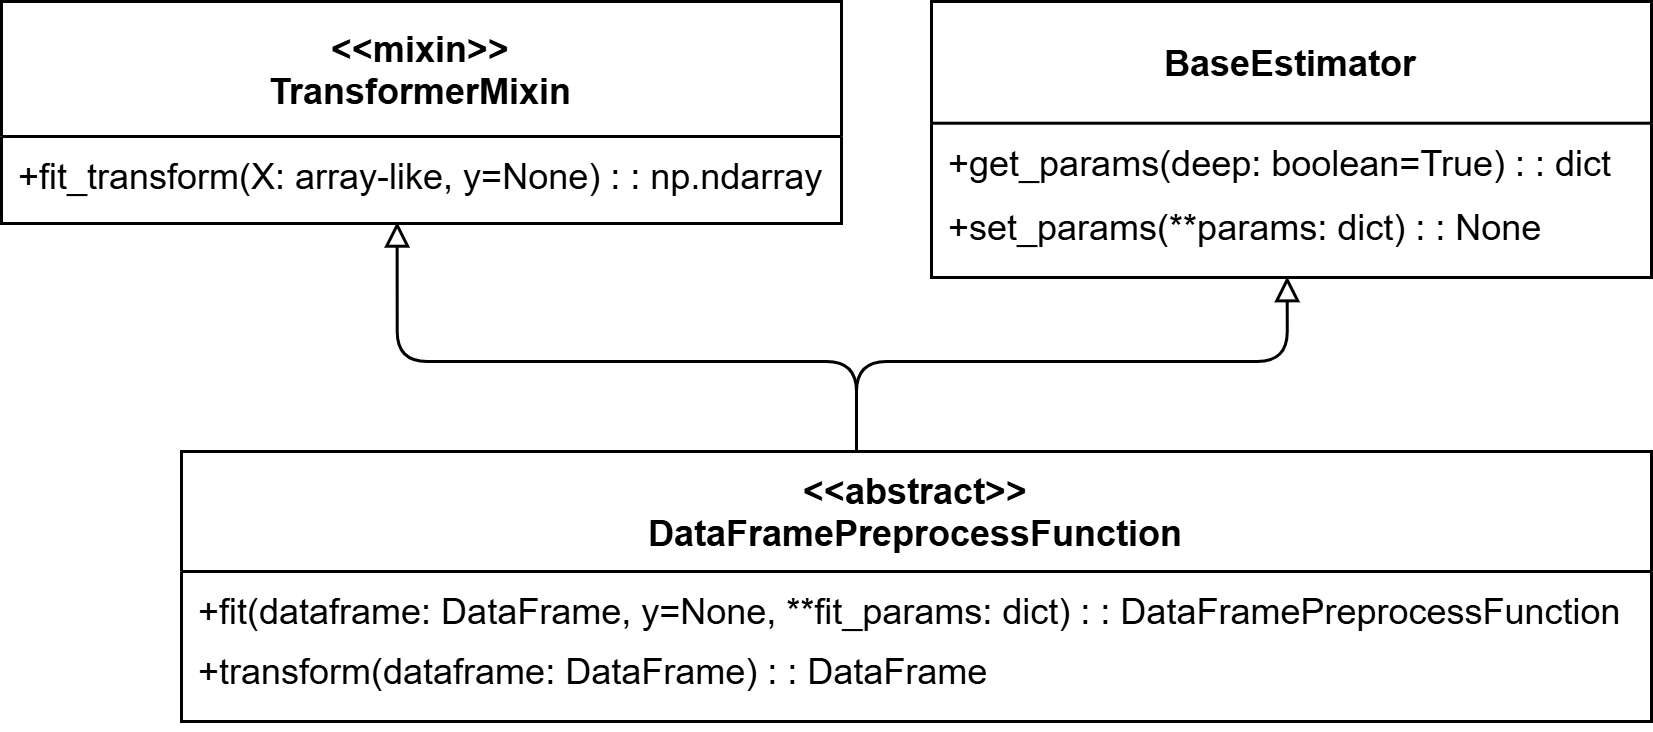
\includegraphics[scale=0.2]{figures/UML/preprocessing/dataframe_preprocess_function.png}
    \caption{Diagramma della classe \texttt{DataFramePreprocessFunction}}
\end{figure}

Tutti i \textit{transformers} della libreria estendono direttamente o indirettamente questa classe per poter implementare i metodi \texttt{fit} e \texttt{transform}. 

Vengono create anche diverse classi per poter raggruppare comportamenti comuni di alcune tipologie di \textit{transformers}:

\begin{itemize}
    \item \texttt{GroupByFunction}: estende \texttt{DataFramePreprocessFunction} e modella l'applicazione di una trasformazione su dati raggruppati (\textit{group-by}). Viene definito il metodo astratto \texttt{\_build\_transform\_function}, applicando il pattern \textit{Template Method}. Questo metodo viene invocato all'interno del metodo \texttt{fit} e restituisce una funzione, che viene salvata come attributo. Questa funzione viene poi utilizzata nel metodo \texttt{transform} sui dati in input trasformandoli.
    
    La classe viene estesa a sua volta da \texttt{Normalizer}, che normalizza vettori per lunghezza unitaria.

    \begin{figure}[H]
        \centering
        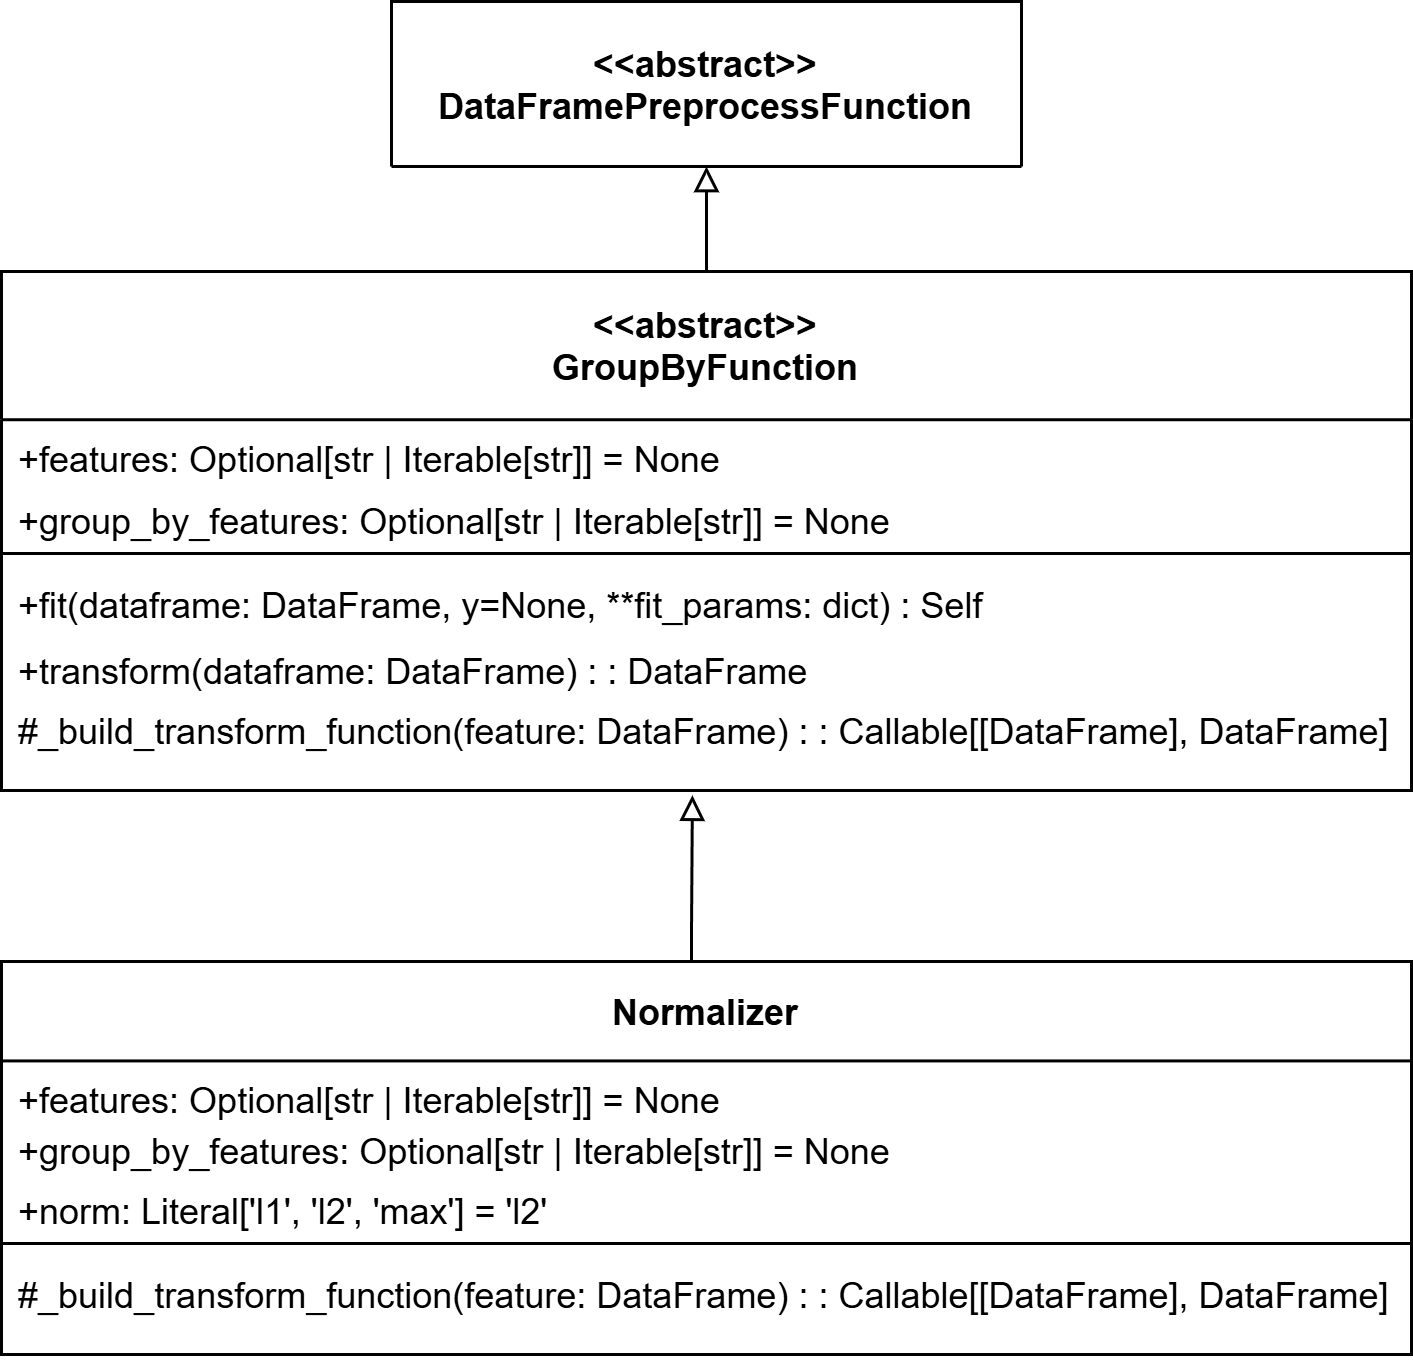
\includegraphics[scale=0.2]{figures/UML/preprocessing/group_by.png}
        \caption{Gerarchia di \texttt{GroupByFunction}}
    \end{figure}

    \item \texttt{InverseTransformer}: classe base per trasformazioni invertibili (che permettono di tornare ai dati originali) grazie alla invocazione al metodo \texttt{inverse\_transform}.
    
    La classe viene estesa a sua volta da \texttt{LabelEncoder}, che codifica etichette categoriali in valori numerici e permette l'inversione.
    
    \begin{figure}[H]
        \centering
        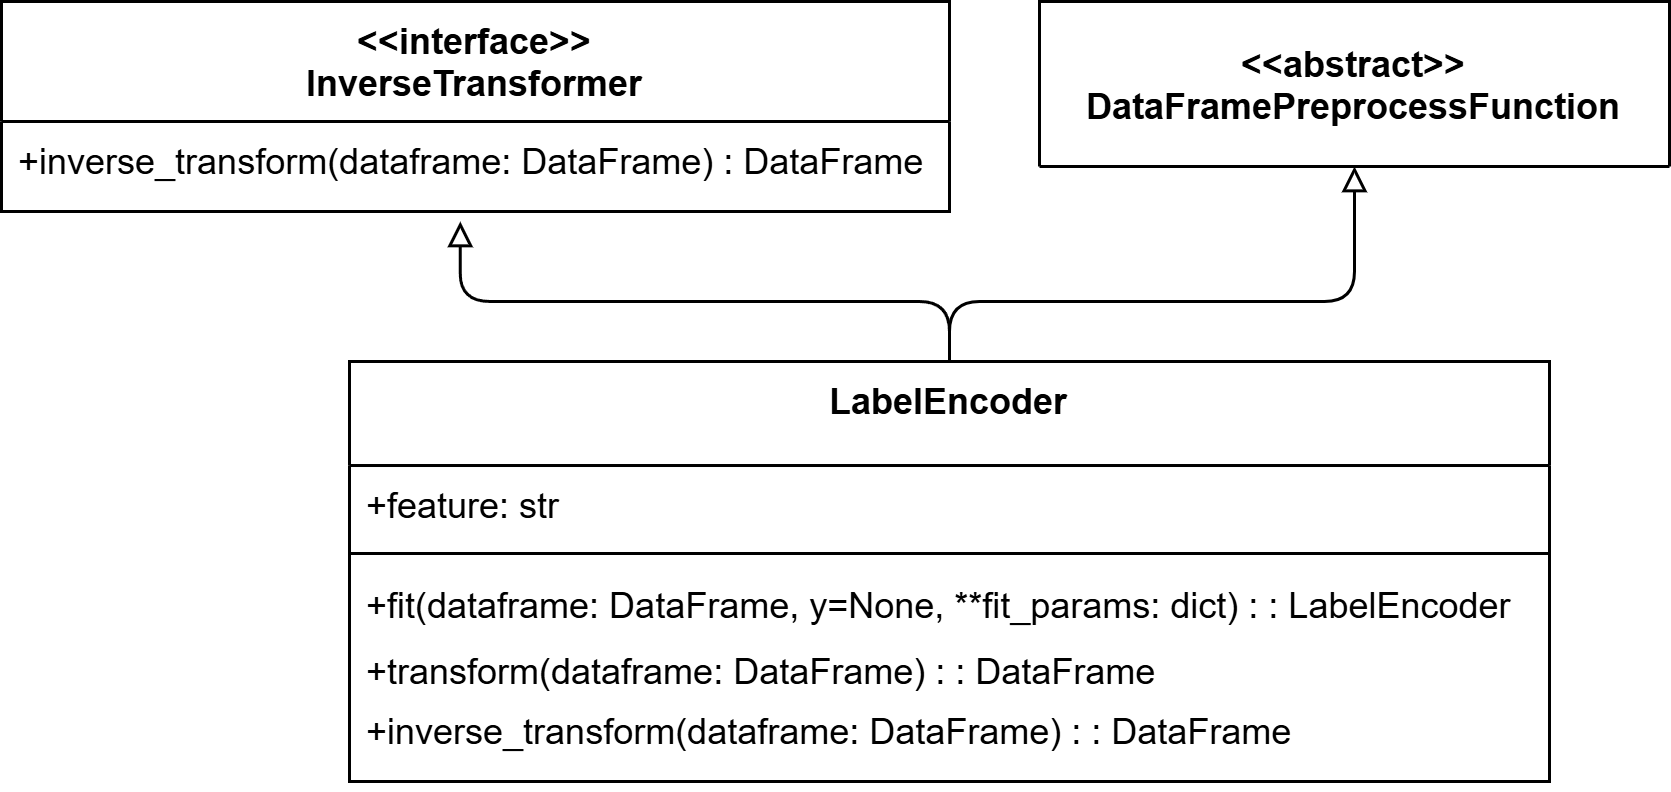
\includegraphics[scale=0.2]{figures/UML/preprocessing/inverse_transformer.png}
        \caption{Gerarchia di \texttt{InverseTransformer}}
    \end{figure}

    \item \texttt{InvertibleGroupByFunction}: estende \texttt{GroupByFunction} e \texttt{InverseTransformer}, permette di invertire le trasformazioni su gruppi. Vengono definiti i metodi astratti \texttt{\_build\_transform\_function} e \texttt{\_build\_inverse\_function}, applicando il pattern \textit{Template Method}, i quali vengono invocati entrambi dentro i metodi \texttt{fit} e restituiscono una funzione ciascuno che vengono salvate come attributi. Queste funzioni vengono poi utilizzate durante l'invocazione dei metodi \texttt{transform} e di \texttt{inverse\_transform} per applicare la trasformazione corrispondente.
    
    La classe viene estesa a sua volta da \texttt{StandardScaler}, che normalizza i dati rendendoli con media $0$ e deviazione standard $1$, e \texttt{MinMaxScaler}, che scala i dati in un intervallo specifico (di solito $[0, 1]$).
    
    \begin{figure}[H]
        \centering
        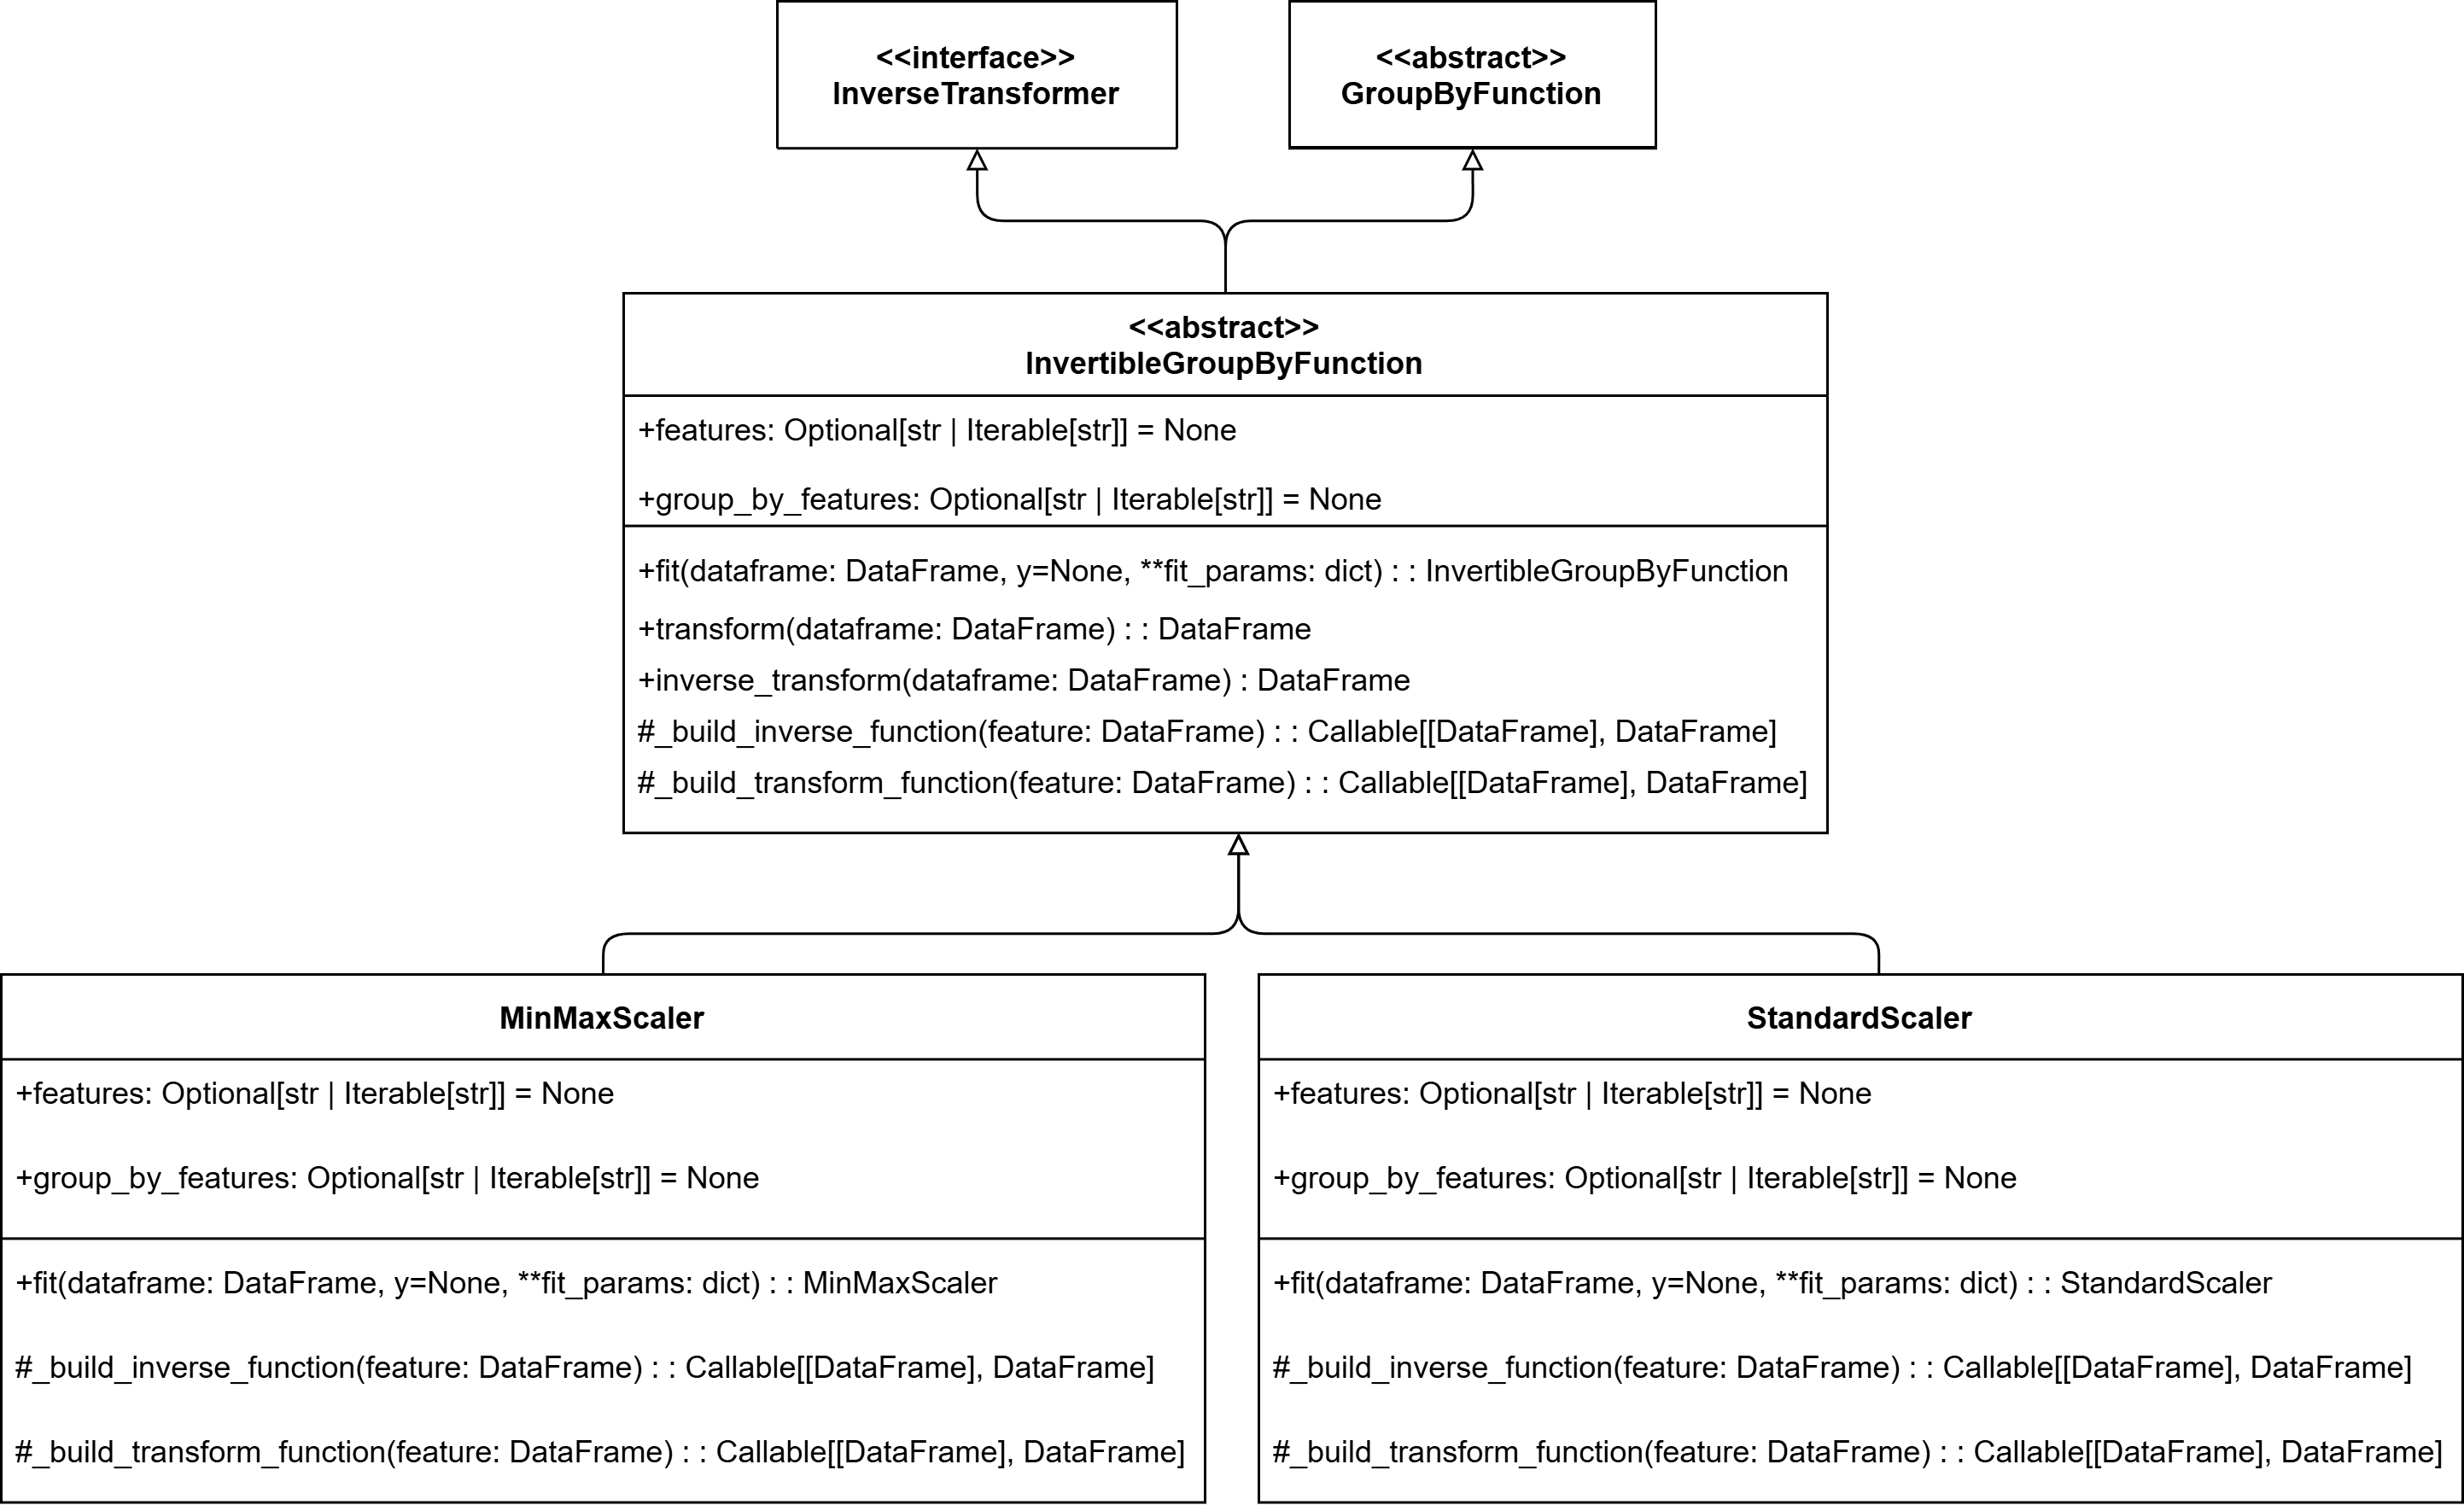
\includegraphics[scale=0.1]{figures/UML/preprocessing/invertible_group_by.png}
        \caption{Gerarchia di \texttt{InvertibleGroupByFunction}}
    \end{figure}
    
    \item \texttt{BinDensity}: estende \texttt{DataFramePreprocessFunction}, si occupa di binning e densità dei dati. Viene definito il metodo astratto \texttt{\_divide} applicando il pattern \textit{Template Method}, il quale viene invocato dentro il metodo \texttt{fit} e restituisce una funzione che viene salvata come attributo. Questa funzione viene poi utilizzata nel metodo \texttt{transform} per applicare la trasformazione corrispondente.
    
    La classe viene estesa a sua volta da \texttt{BinThreshold}, che effettua \textit{binning} basato su una soglia di frequenza, e \texttt{BinCumulative}, che effettua \textit{binning} basato su cumulativi di distribuzione.
    \begin{figure}[H]
        \centering
        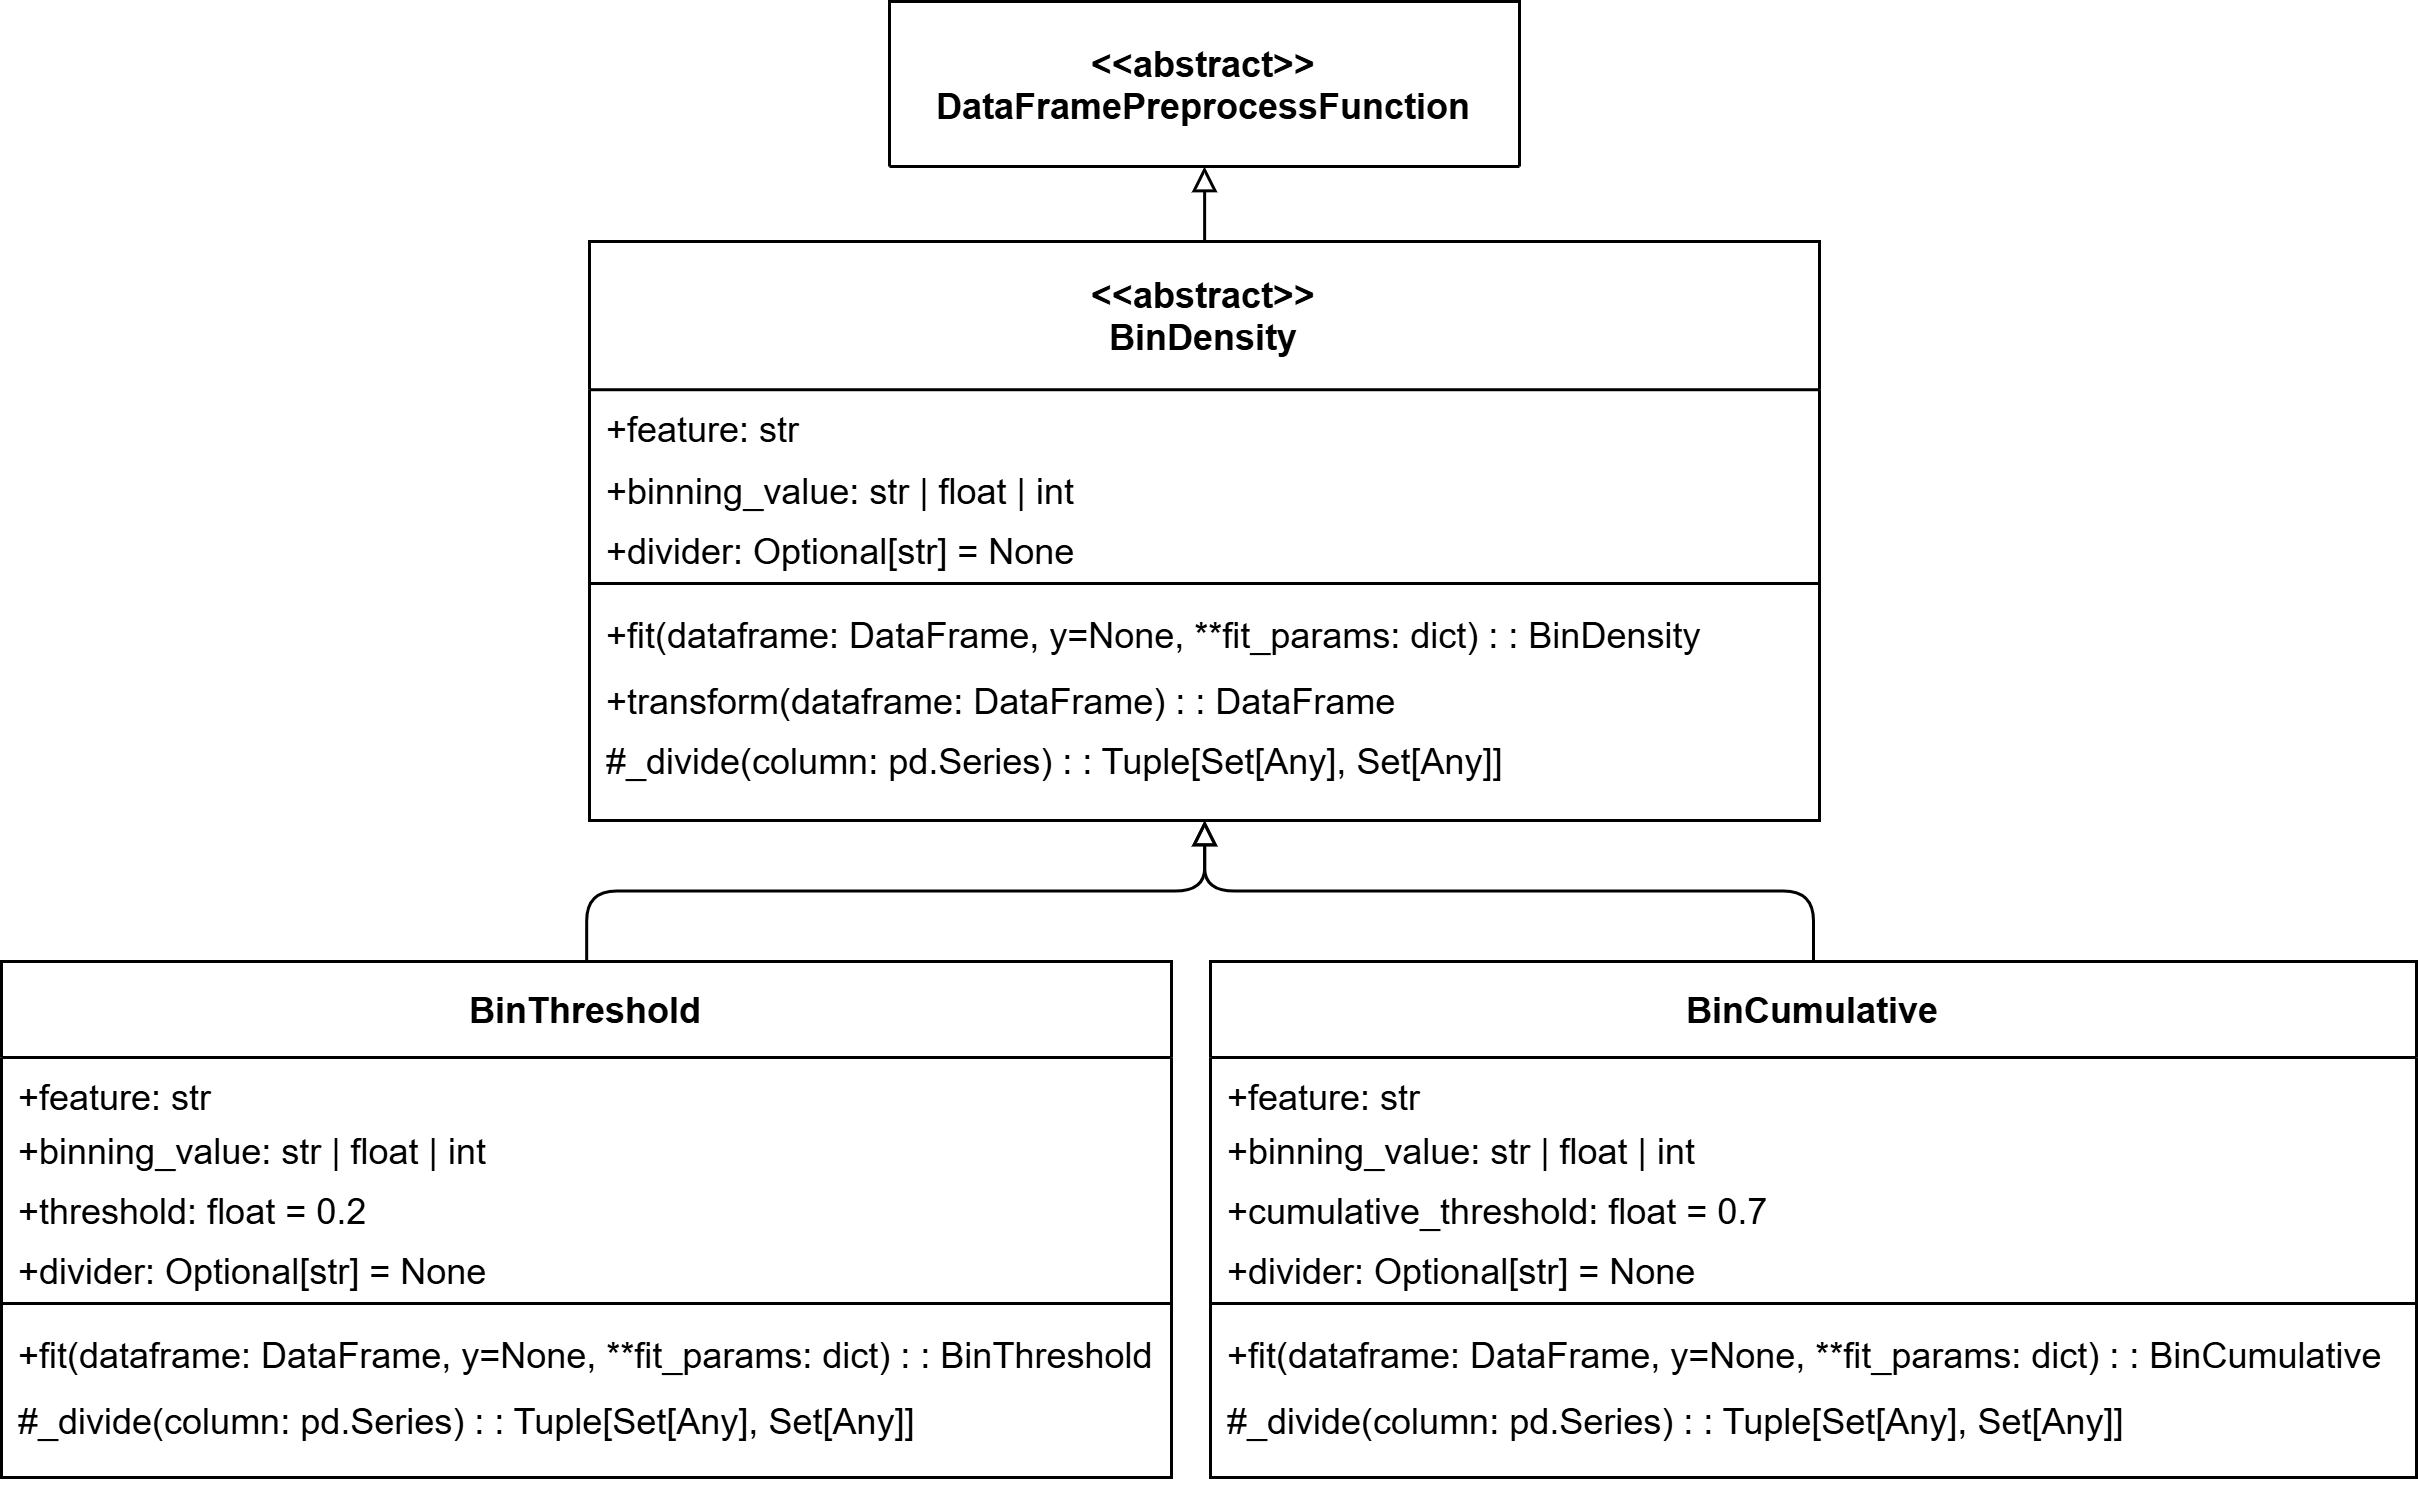
\includegraphics[scale=0.10]{figures/UML/preprocessing/bin_density.png}
        \caption{Gerarchia di \texttt{BinDensity}}
    \end{figure}
\end{itemize}

\subsection{Pipeline pattern}

Si è deciso di utilizzare il \textit{pipeline pattern} per l'applicazione dei \textit{transformer} ai dati. Questo pattern è una struttura architetturale in cui una serie di elaborazioni vengono applicate sequenzialmente a un flusso di dati, in questo caso il \textit{dataset} del tipo \textit{DataFrame}. Ogni stadio della \textit{pipeline} prende in input l'output dello stadio precedente, eseguendo una trasformazione. Ogni componente della \textit{pipeline} è modulare, indipendente, non modifica i valori in input (genera una copia in output) né causa \textit{side effect}. L'elaborazione delle trasformazioni avviene in sequenza ed è possibile modificare sia l'ordine delle trasformazioni che le trasformazioni stesse. In caso ci fosse un errore in una delle trasformazioni la \textit{pipeline} non va a buon fine.

\begin{figure}[H]
    \centering
    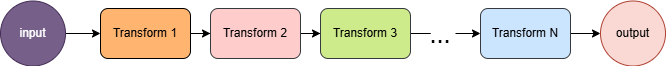
\includegraphics[scale=0.45]{figures/pipeline.png}
    \caption{\textit{Pipeline pattern}}
    \label{fig:pipeline}
\end{figure}

La pipeline, anch'essa una \textit{DataFramePreprocessFunction} che applica tutte le trasformazioni specificate, è definita come \texttt{PreprocessPipeline}.

\begin{figure}[H]
    \centering
    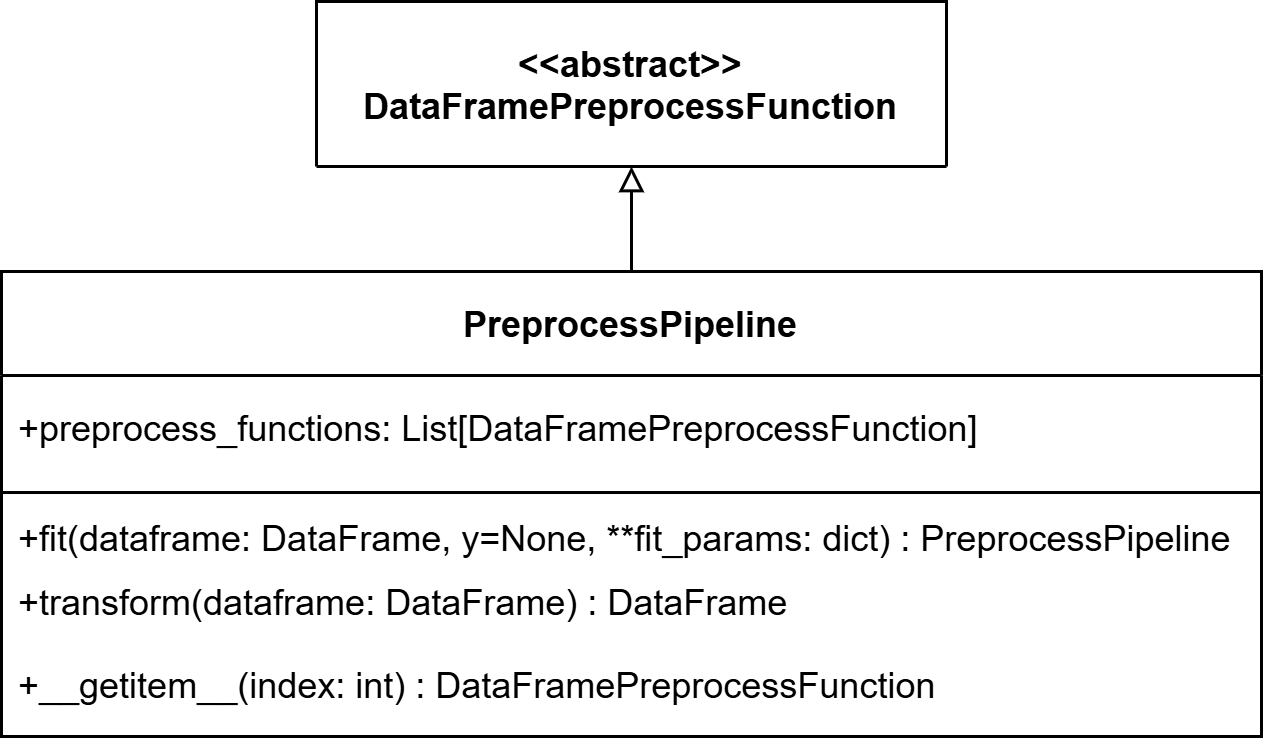
\includegraphics[scale=0.2]{figures/UML/preprocessing/preprocess_pipeline.png}
    \caption{Diagramma della classe \texttt{PreprocessPipeline}}
    \label{fig:preprocess_pipeline}
\end{figure}

Un esempio di utilizzo è:

\begin{lstlisting}[caption=esempio di utilizzo di \texttt{PreprocessPipeline}]
pipeline = PreprocessPipeline([
    Drop('timestamp'),
    Bin('rating', bins=5),
    ...
])
preprocessed_dataset = pipeline.fit_transform(dataset) 
\end{lstlisting}

\subsection{Tranformers}

Un elenco dei \textit{transformers} che estendono direttamente la classe \\
\texttt{DataFramePreprocessFunction} e una descrizione delle operazioni che svolgono:

\begin{itemize}
    \item \texttt{Select}: seleziona specifiche colonne
    \item \texttt{FillNa}: riempie i valori mancanti
    \item \texttt{Filter}: filtra le righe secondo una funzione di filtro
    \item \texttt{Drop}: rimuove colonne specificate
    \item \texttt{Rename}: rinomina colonne
    \item \texttt{Update}: aggiorna dati esistenti
    \item \texttt{Round}: arrotonda valori numerici a un numero specifico di cifre decimali
    \item \texttt{Bin}: crea categorie (\textit{bin}) da valori continui in una colonna
    \item \texttt{ExtractDate}: estrae componenti della data da una colonna \textit{datetime}
    \item \texttt{DropNa}: elimina righe con valori mancanti in colonne specifiche
    \item \texttt{DropDuplicates}: rimuove righe duplicate
    \item \texttt{Cycle}: calcola valori ciclici (es. per data o tempo)
    \item \texttt{Clip}: limita i valori numerici entro un intervallo specificato
    \item \texttt{Map}: mappa i valori di una colonna usando una funzione o dizionario
    \item \texttt{OneHotEncode}: codifica variabili categoriali in variabili \textit{dummy} (\textit{one-hot})
    \item \texttt{Condense}: aggrega dati raggruppandoli e concatenandoli
    \item \texttt{ToCOOMatrix}: trasforma dati in una matrice sparsa in rappresentazione \textit{COO} (sempre nel tipo \textit{DataFrame})
\end{itemize}

\begin{figure}[H]
    \centering
    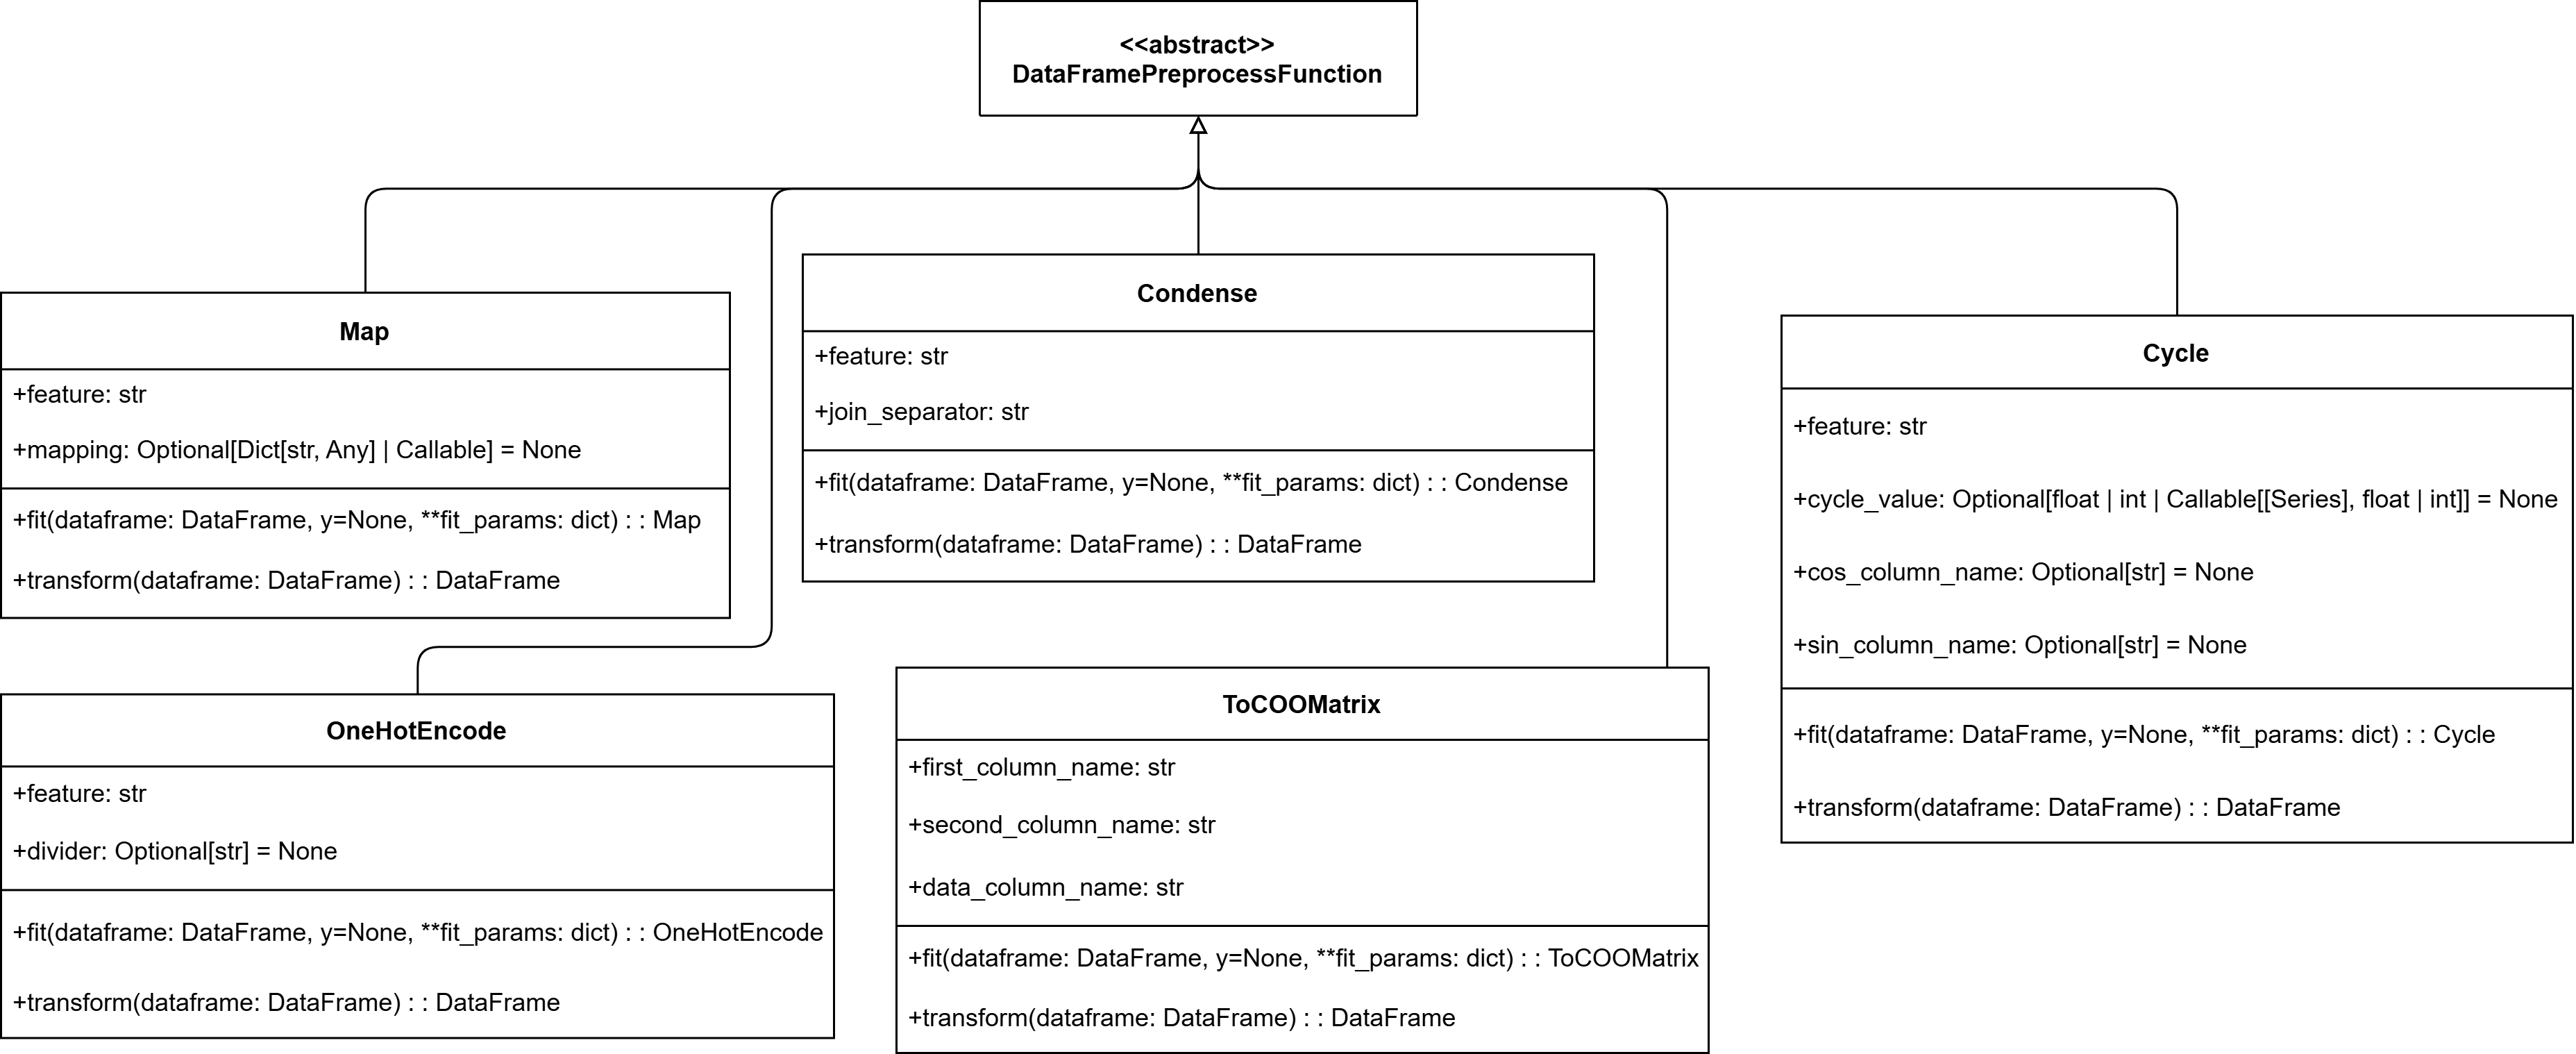
\includegraphics[angle=90, scale=0.14]{figures/UML/preprocessing/direct_1.png}
    \caption{Diagrammi delle classi \texttt{Map}, \texttt{Condense}, \texttt{Cycle}, \\ \texttt{OneHotEncode}, \texttt{ToCOOMatrix}}

\end{figure}\begin{figure}[H]
    \centering
    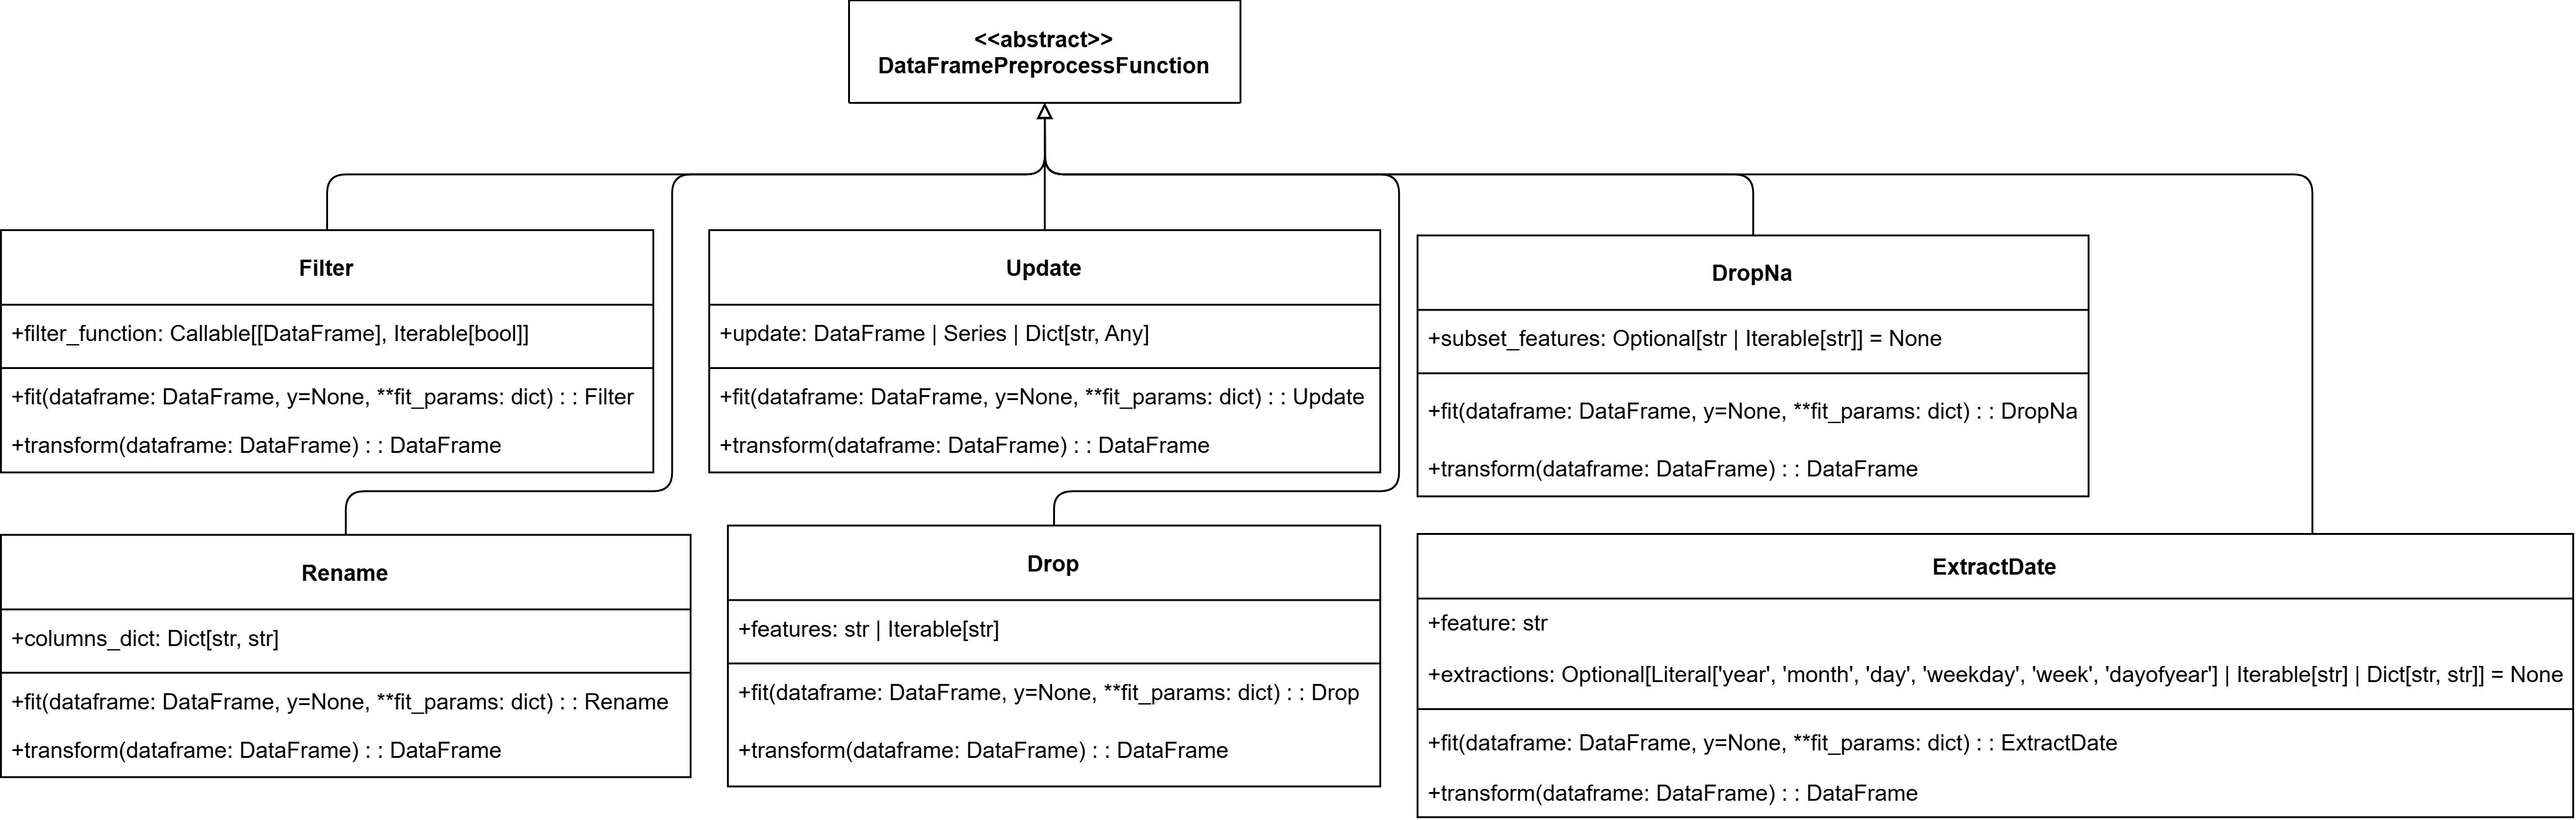
\includegraphics[angle=90, scale=0.13]{figures/UML/preprocessing/direct_2.png}
    \caption{Diagrammi delle classi \texttt{Filter}, \texttt{Update}, \texttt{DropNa}, \texttt{Rename}, \texttt{Drop}, \texttt{ExtractDate}}

\end{figure}\begin{figure}[H]
    \centering
    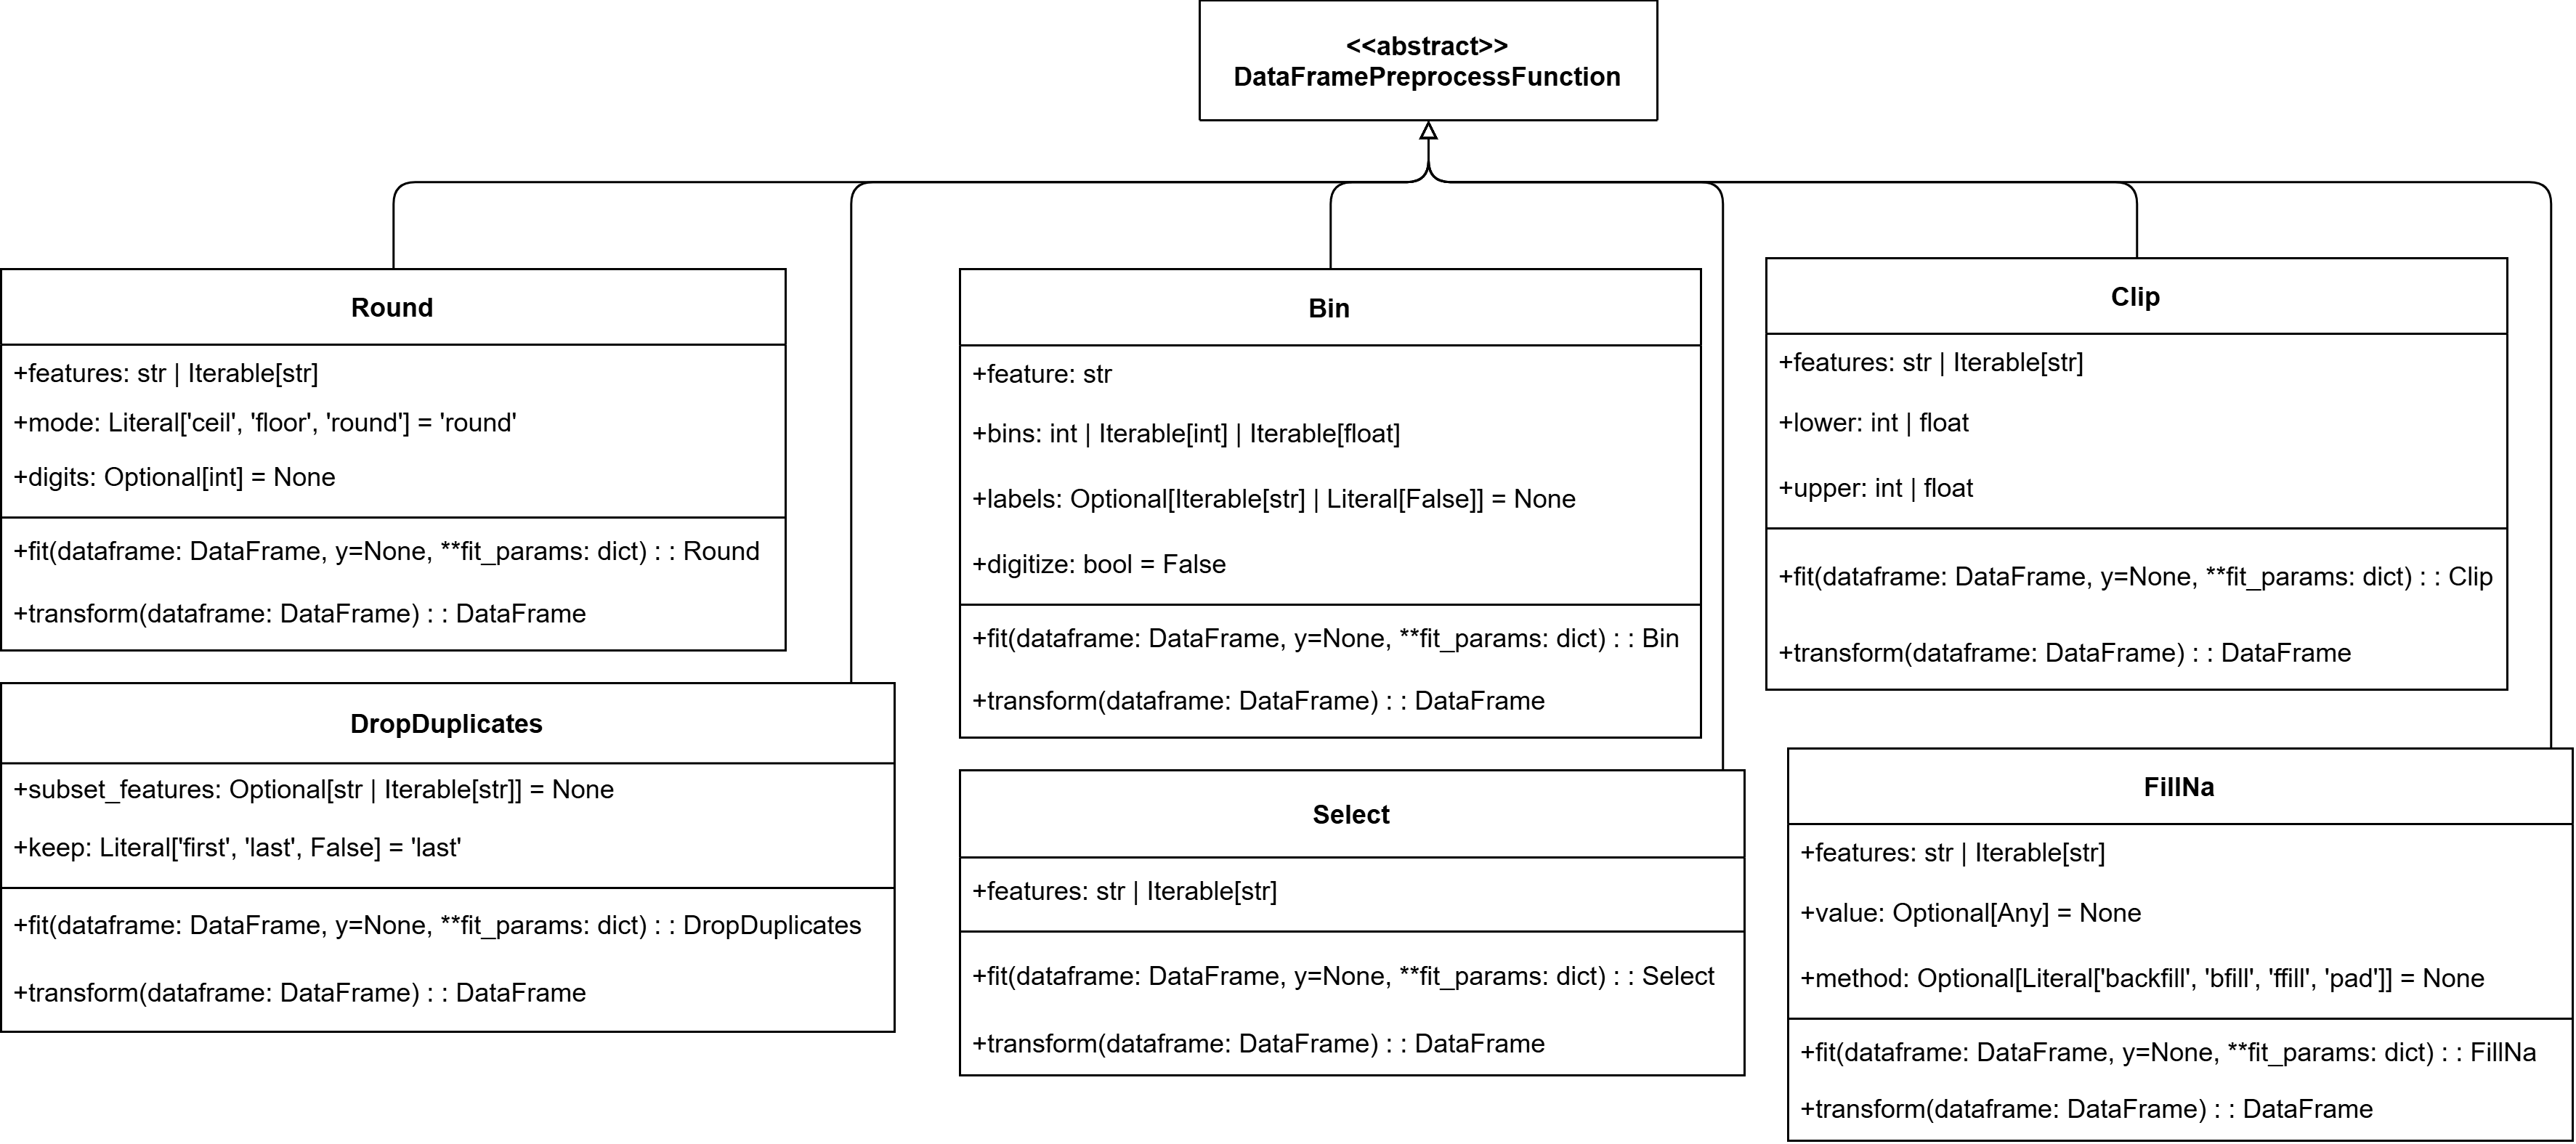
\includegraphics[angle=90, scale=0.15]{figures/UML/preprocessing/direct_3.png}
    \caption{Diagrammi delle classi \texttt{Round}, \texttt{Bin}, \texttt{Clip}, \texttt{DropDuplicates}, \texttt{Select}, \texttt{FillNa}}
\end{figure}

\section{Models}
Il modulo comprende l'insieme delle classi dei modelli di \textit{recommendation}.

Per i modelli che gestiscono feedback espliciti sono presenti i seguenti algoritmi:

\begin{itemize}
    \item \textit{SVD}~\ref{svd}
    \item \textit{SVD++}~\ref{svdpp}
    \item \textit{NFM}~\ref{nmf}
    \item \textit{KNN con baseline}~\ref{knn}
    \item \textit{CoClustering}~\ref{coclustering}
    \item \textit{SlopeOne}~\ref{slopeone}
\end{itemize}

mentre per quelli che gestiscono feedback impliciti:

\begin{itemize}
    \item \textit{ALS}~\ref{als} 
    \item \textit{BRP}~\ref{bpr} 
    \item \textit{LMF}~\ref{lmf}
    \item \textit{LightFM}~\ref{lightfm}  
\end{itemize}

Per ogni algoritmo, la libreria applica il pattern \textit{Adapter} per rendere compatibili i modelli con la libreria \textit{Scikit-learn}.

\subsection{Compatibilità con Scikit-learn, modelli}\label{compatibilita_sklearn}

Per definire un modello custom compatibile con la suite di \textit{Scikit-learn} occorre seguire alcuni requisiti che possono essere variabili. Vengono presentate le scelte effettuate per la libreria e che ogni modello deve rispettare:

\begin{itemize}
    \item estendere la classe \texttt{BaseEstimator}
    \item implementare il metodo \texttt{fit} che abbia almeno come parametri:
    \begin{itemize}
        \item \texttt{X} di tipo \textit{array-like}, \textit{sparse matrix} o \textit{DataFrame}
        \item \texttt{y} che in questo caso viene sempre inizializzata con un valore di default \texttt{None} e che non viene utilizzata ma che viene specificata per convenzione per avere una API coerente
    \end{itemize}
    \item implementare il metodo \texttt{predict} che abbia almeno come parametro X di tipo \textit{array-like}, \textit{sparse matrix} o \textit{DataFrame} e che restituisca come risultato un \textit{NumPy array}
    \item tutti i campi devono essere pubblici e chiamarsi allo stesso modo dei parametri del costruttore
    \item non ci devono essere computazioni all'interno del costruttore ma solamente le inizializzazioni dei campi
    \item una volta che il metodo \texttt{fit} viene invocato devono essere valorizzati parametri che terminano con il carattere "\_" (e.g. \texttt{model.item\_factors\_} e \\ \texttt{model.user\_factors\_})
    \item inserire, all'interno del metodo \texttt{predict}, un controllo che verifichi che il modello sia stato addestrato, utilizzando la funzione \texttt{check\_is\_fitted}. Questa funzione verifica la presenza di almeno un attributo il cui nome termini con il carattere ``\_'' (convenzionalmente utilizzato da \textit{Scikit-learn} per indicare che l'attributo è stato appreso durante il training). In caso contrario, viene sollevata un'eccezione di tipo \texttt{NotFittedError}
\end{itemize}

I modelli possono, in base alle necessità, aggiungere parametri aggiuntivi alle funzioni di \texttt{fit} e di \texttt{predict}, per esempio eventuali \texttt{user\_features} o \texttt{item\_features}.

\subsection{Salvataggio modelli}

Viene definita l'interfaccia \texttt{PersistableModel} che espone il metodo \texttt{save} per il salvataggio dei modelli. Il metodo riceve come parametro \texttt{fileobj\_or\_path} che corrisponde al nome del file (che include anche il percorso, tipo \texttt{str}) oppure un oggetto file aperto (tipo \texttt{io.IOBase}) su cui salvare il modello.

\begin{figure}[H]
    \centering
    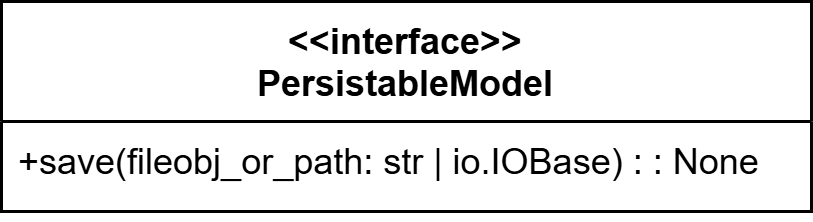
\includegraphics[scale=0.3]{figures/UML/models/persistable_model.png}
    \caption{Diagramma del'interfaccia \texttt{PersistableModel}}
\end{figure}

Per il caricamento da file ogni modello implementerà autonomamente un metodo \texttt{load}, che potrà essere tipo \textit{classmethod} oppure un \textit{staticmethod}.

\subsection{Model fit data}\label{model_fit_data}

I vari modelli possono essere addestrati con il metodo \texttt{fit} su diversi formati di dati, purché rispettino i vincoli sopra descritti. Per i modelli sviluppati si è deciso un formato standard. La prima colonna è composta dagli \textit{user\_id}, che corrispondono agli id degli \textit{user}, la seconda colonna all'\textit{item\_id}, che corrispondono agli id degli \textit{item}, e le eventuali colonne successive a informazioni aggiuntive sull'interazione, per esempio il \textit{rating} o il \textit{timestamp}. Le uniche informazioni obbligatorie sono quindi solamente le coppie (\textit{user\_id}, \textit{item\_id}). I modelli possono in modo indipendente introdurre eventuali vincoli sui dati in input.

Un esempio di input in formato \textit{DataFrame}:

\begin{table}[H]
    \centering
    \begin{tabular}{|c|c|c|c|}
    \hline
    \textbf{user\_id} & \textbf{item\_id} & \textbf{rating} & \textbf{timestamp} \\
    \hline
        101 & 501 & 4.0 & 2021-03-14 08:23:45 \\
        102 & 502 & 5.0 & 2022-07-19 16:45:10 \\
        103 & 503 & 3.5 & 2020-11-03 03:12:00 \\
        104 & 504 & 2.0 & 2019-01-27 22:58:36 \\
        105 & 505 & 4.5 & 2023-09-05 13:37:21 \\
    \hline
    \end{tabular}
    \caption{Esempio di input con due colonne extra per i \textit{rating} e il \textit{timestamp}}
    \label{tab:ratings}
\end{table}

\subsubsection{Ids}

Ogni volta che si fa riferimento ad un id, che sia \texttt{user\_id} o \texttt{item\_id}, si considera che il tipo sia \texttt{int} oppure \texttt{str}. 

\subsection{Model predict data}\label{model_predict_data}

I vari modelli possono predire il \textit{rating} o lo \textit{score} con il metodo \texttt{predict} su diversi formati di dati, purché rispettino i vincoli sopra descritti. Il formato standard deciso è identico a quello utilizzato per l'addestramento~\ref{model_fit_data}. I modelli possono in modo indipendente introdurre eventuali vincoli sui dati in input.

In questo caso però il modello utilizza la singola coppia (\textit{user\_id}, \textit{item\_id}) alla quale viene associato un \textit{rating} o lo \textit{score} in base al tipo di modello utilizzato, rispettivamente per feedback espliciti e per feedback impliciti. Se, per esempio, vengono dati in input al modello, che gestisce feedback impliciti, cinque coppie (\textit{user\_id}, \textit{item\_id}) quest'ultimo restituisce un \textit{NumPy array} di cinque valori, ciascuno corrispondente allo \textit{score} ottenuto da ciascuna coppia. Se si vuole ottenere il \textit{ranking} occorre ordinare gli \textit{score} ottenuti in ordine decrescente. Se si vuole calcolare \textit{rating} o lo \textit{score}, dati un insieme $U$ di \textit{user} e $I$ di \textit{item}, occorre dare in input al metodo \texttt{predict} tutte le combinazioni $\left\{(u, i) \mid u \in U,\; i \in I \right\}$.

Un esempio di input in formato \textit{DataFrame} e di output in formato \textit{NumPy array}:

\begin{table}[H]
    \centering
    \begin{minipage}{0.6\textwidth}
        \centering
        \begin{tabular}{|c|c|c|c|}
        \hline
        \textbf{user\_id} & \textbf{item\_id} \\
        \hline
            101 & 501 \\
            102 & 502 \\
            103 & 503 \\
            104 & 504 \\
            105 & 505 \\
        \hline
        \end{tabular}
    \end{minipage}%
    \hfill
    \begin{minipage}{0.3\textwidth}
        \centering
        \begin{tabular}{|c|}
        \hline
        0.97 \\
        -0.12 \\
        1.02 \\
        0.08 \\
        0.55 \\
        \hline
        \end{tabular}
    \end{minipage}
    \caption{Esempio output restituito dal modello che gestisce feedback impliciti}
    \label{tab:ratings_with_score}
\end{table}

Importante considerare che gli \textit{score}, generati dai modelli impliciti, singolarmente non hanno alcun significato ma vengono utilizzati solamente per definire un ordinamento.

\subsection{Similarità user-user o item-item}

I modelli posso estendere l'interfaccia \texttt{SimilarityModel} che espone due metodi per calcolare la similarità tra \textit{users-users} e tra \textit{items-items}. Solitamente il calcolo include l'utilizzo di vettori \textit{embedding} appresi durante l'addestramento. Sono strumento che permette di effettuare \textit{up-selling}, trovando \textit{item} simili si può proporre una versione più costosa o avanzata.

Il metodo \texttt{similar\_users} ha i seguenti parametri:

\begin{itemize}
    \item \texttt{user\_id} (singolo id o \texttt{NumPy array} o \texttt{Series}): id dello \textit{user} o lista di id per cui si desidera trovare \textit{user} simili
    \item \texttt{N} (\texttt{int}): numero di \textit{user} simili da restituire. Il valore di default è 10
    \item \texttt{filter\_users} (\texttt{NumPy array} o \texttt{Series}): lista di id di \textit{user} da escludere dai risultati
    \item \texttt{users} (\texttt{NumPy array} o \texttt{Series}): lista di id di \textit{users} da includere nei risultati. Non può essere utilizzata insieme a \texttt{filter\_users}
\end{itemize}

Il metodo \texttt{similar\_items} ha i seguenti parametri:
\begin{itemize}
    \item \texttt{item\_id} (singolo id o \texttt{NumPy array} o \texttt{Series}): id dell'\textit{item} o lista di id per cui si desidera trovare \textit{item} simili
    \item \texttt{N} (\texttt{int}): numero di \textit{item} simili da restituire. Il valore di default è 10
    \item \texttt{filter\_items} (\texttt{NumPy array} o \texttt{Series}): lista di id di \textit{item} da escludere dai risultati
    \item \texttt{items} (\texttt{NumPy array} o \texttt{Series}): lista di id di \textit{item} da includere nei risultati. Non può essere utilizzata insieme a \texttt{filter\_items}
\end{itemize}

Entrambi i metodo restituiscono un \textit{NumPy array} di (\textit{user\_id}/\textit{item\_id}, \textit{score}), dove lo \textit{score} indica quanto sono simili. In base al modello utilizzato il valore potrebbe essere compreso in un intervallo oppure no.

\begin{figure}[H]
    \centering
    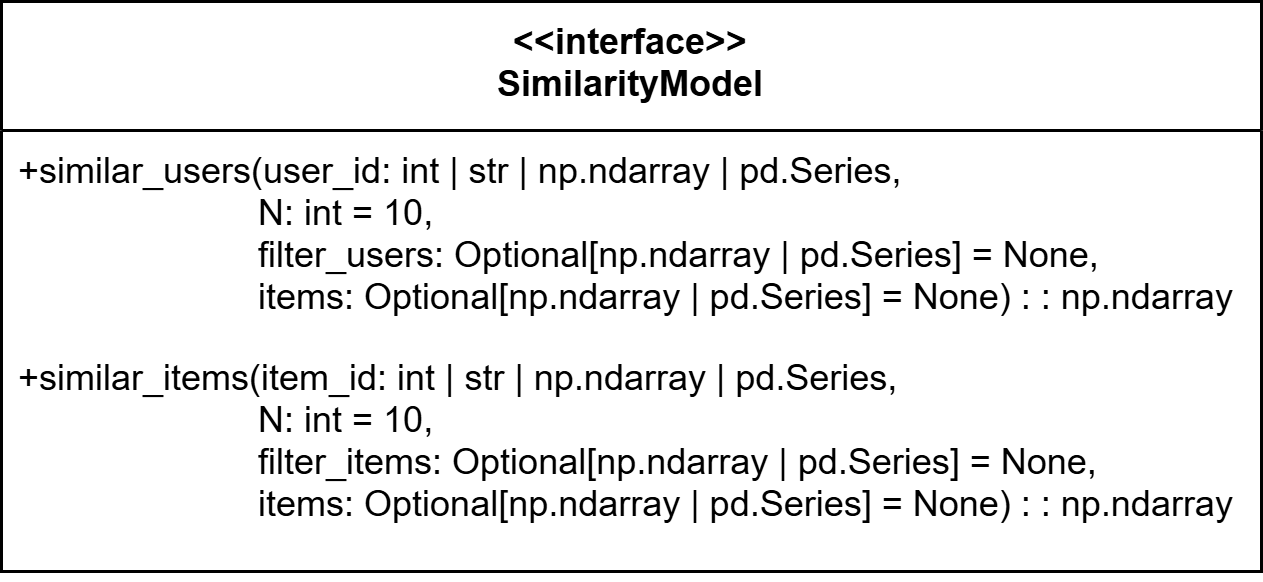
\includegraphics[scale=0.25]{figures/UML/models/similarity_model.png}
    \caption{Diagramma dell'interfaccia \texttt{SimilarityModel}}
\end{figure}

Importante inserire, all'interno del due metodi, un controllo che verifichi che il modello sia stato addestrato, utilizzando la funzione \texttt{check\_is\_fitted} come per il metodo \texttt{predict}~\ref{compatibilita_sklearn}.

\subsection{Modelli Surprise}

Viene definita la classe astratta \texttt{SurpriseModel} che estende \texttt{BaseEstimator} e \texttt{PersistableModel} e che gestisce il comportamento comune della \texttt{fit} e della \texttt{predict} di tutti i modelli della libreria \textit{Surprise}. Viene definito il metodo astratto \texttt{\_fit\_surprise\_model}, applicando il pattern \textit{Template Method}. Così facendo, l'implementazione di ogni modello deve definire solamente le modalità di addestramento del modello della libreria \textit{Surprise} e quali attributi, il cui nome termina con il carattere "\_", vengono appresi.

\begin{figure}[H]
    \centering
    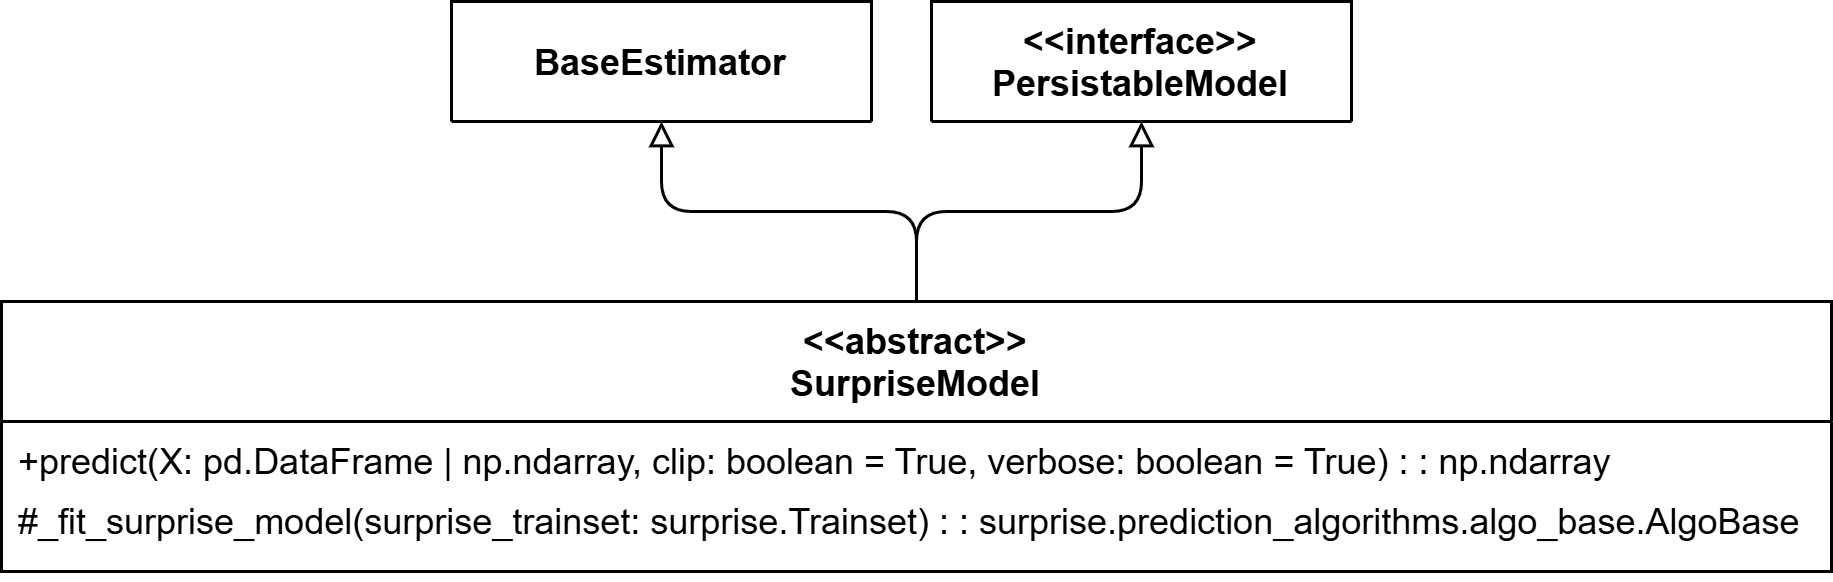
\includegraphics[scale=0.17]{figures/UML/models/surprise_model.png}
    \caption{Diagramma della classe astratta \texttt{SurpriseModel}}
\end{figure}'


La classe viene estesa creando i vari adapter dei modelli:

\begin{itemize}
    \item \texttt{SVD}
    \item \texttt{SVDpp}
    \item \texttt{KNNBaseline}
    \item \texttt{SlopeOne}
    \item \texttt{CoClustering}
\end{itemize}

Ogni modello riceve nel costruttore gli stessi parametri del modello originale della libreria \textit{Surprise}.

Tutti i modelli sopra elencati gestiscono feedback espliciti e quindi i valori restituiti dal metodo \textit{predict} corrispondono a \textit{score}.


\begin{figure}[H]
    \centering
    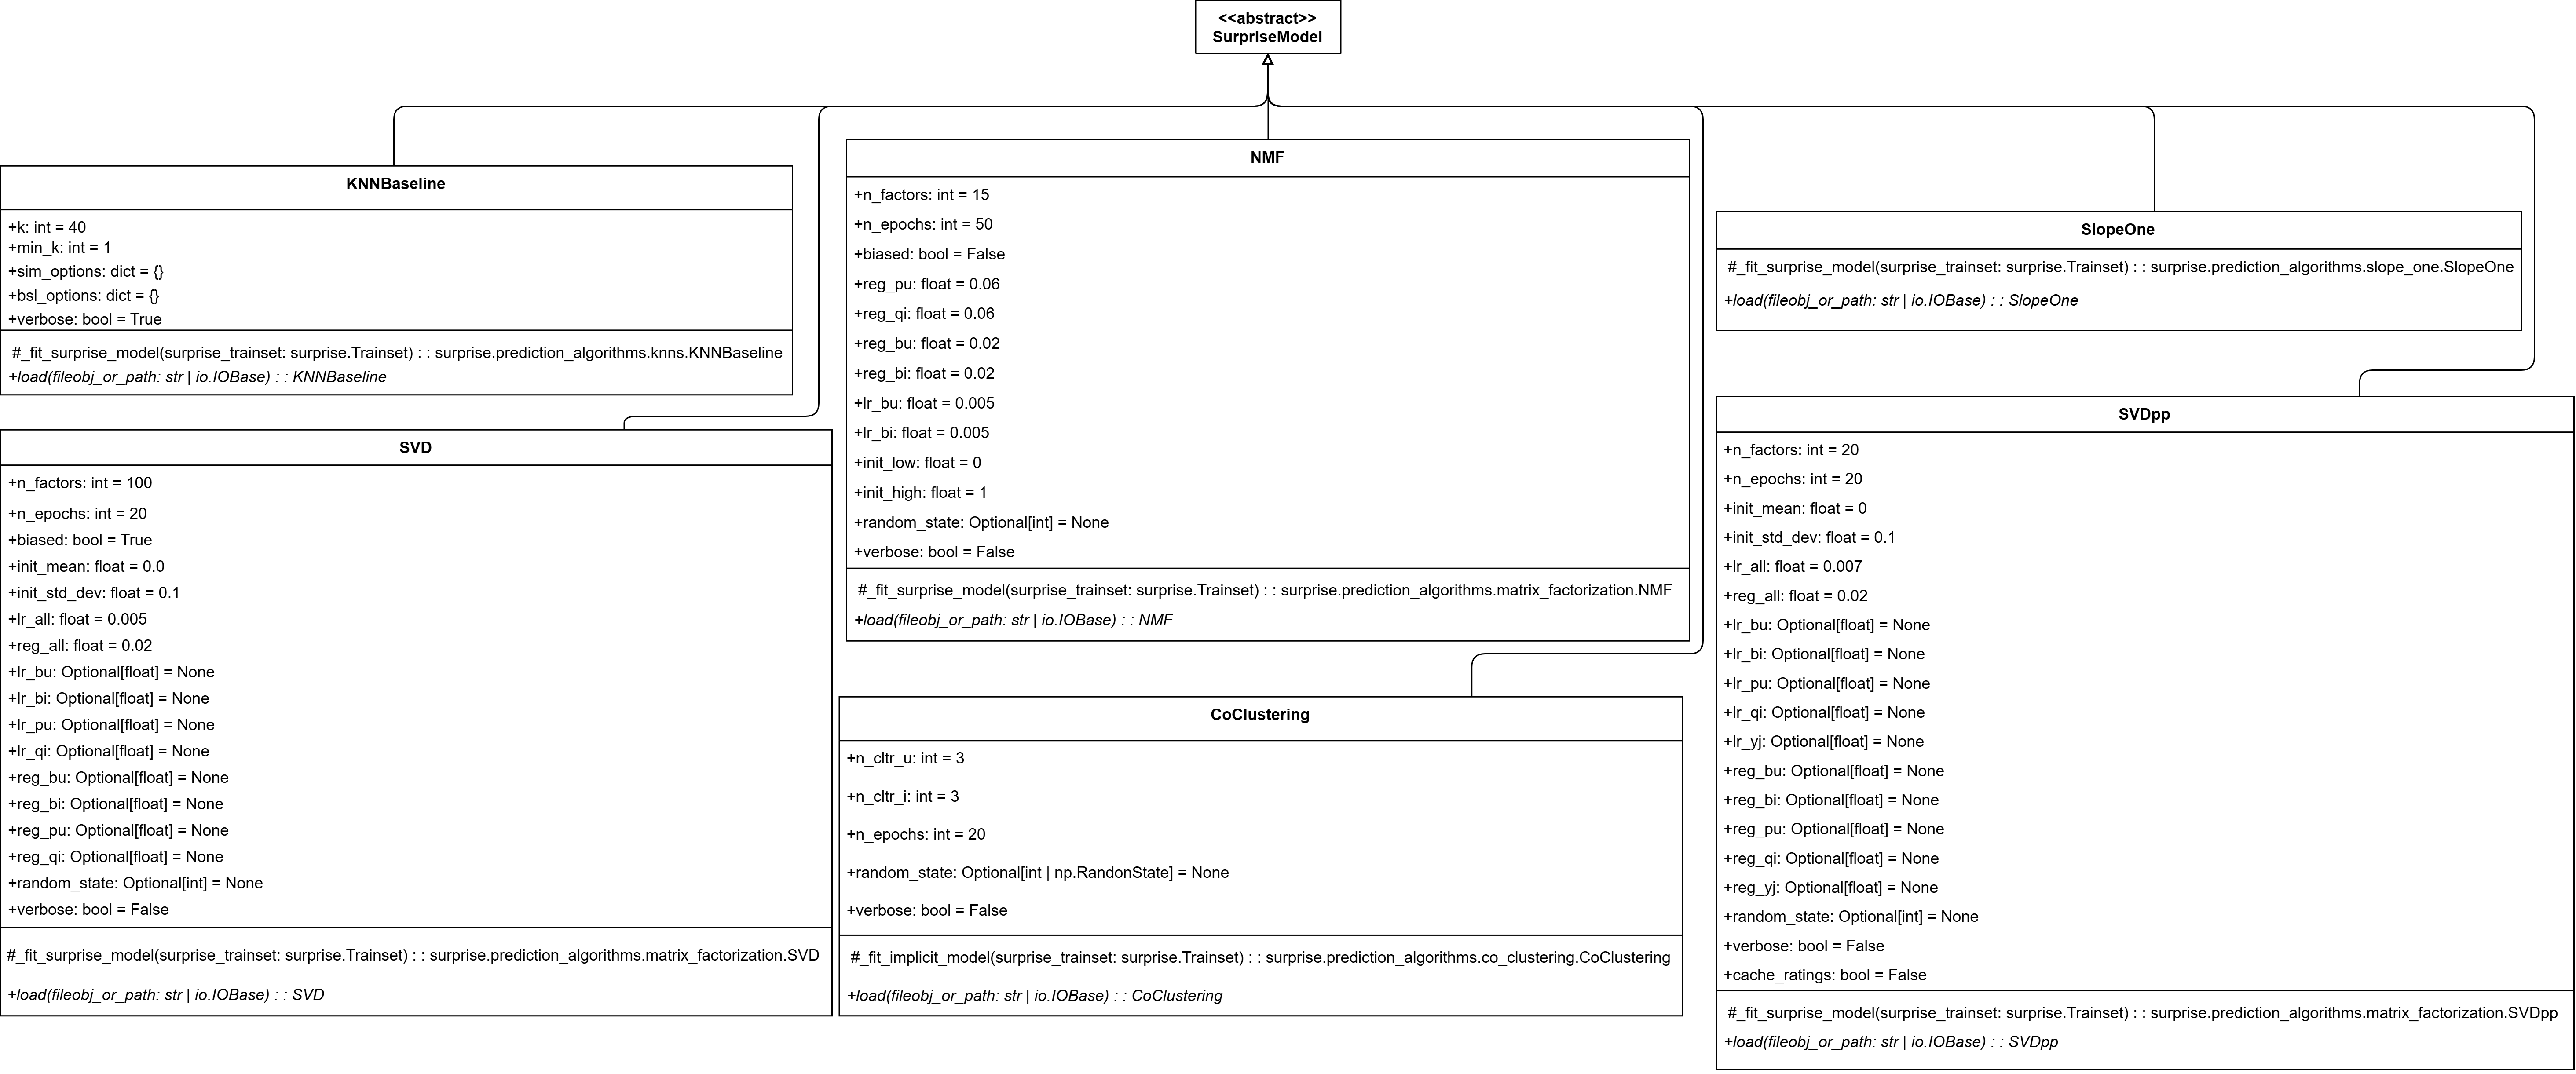
\includegraphics[angle=90, scale=0.09]{figures/UML/models/surprise_models.png}
    \caption{Diagrammi dei modelli di \textit{Surprise}}
\end{figure}

\subsubsection{Modifiche ai metodi}

Il metodo \texttt{predict} di questi modelli può riceve due parametri extra:

\begin{itemize}
    \item \texttt{clip} (\texttt{boolean}): indica se limitare la stima all'interno della scala di valutazione. Ad esempio, se $\hat{r}_{ui} = 5.5$ mentre la scala di valutazione è $[1, 5],$ allora $\hat{r}_{ui}$ viene impostato a 5. Lo stesso vale se $\hat{r}_{ui} < 1.$ Il valore di default è \texttt{True}
    \item \texttt{verbose} (\texttt{boolean}): indica se stampare i dettagli della previsione. Il valore di default è \texttt{False}
\end{itemize}

\subsection{Modelli Implicit}

Viene definita la classe astratta \texttt{ImplicitModel} che estende \texttt{BaseModel},\\ \texttt{PersistableModel} e \texttt{SimilarityModel} e che gestisce il comportamento comune della \texttt{fit} e della \texttt{predict} di tutti i modelli della libreria \textit{Implicit}. Viene definito il metodo astratto \texttt{\_fit\_implicit\_model}, applicando il pattern \textit{Template Method}. Così facendo, l'implementazione di ogni modello deve definire solamente le modalità di addestramento del modello della libreria \textit{Implicit} e quali attributi, il cui nome termina con il carattere "\_", vengono appresi.

\begin{figure}[H]
    \centering
    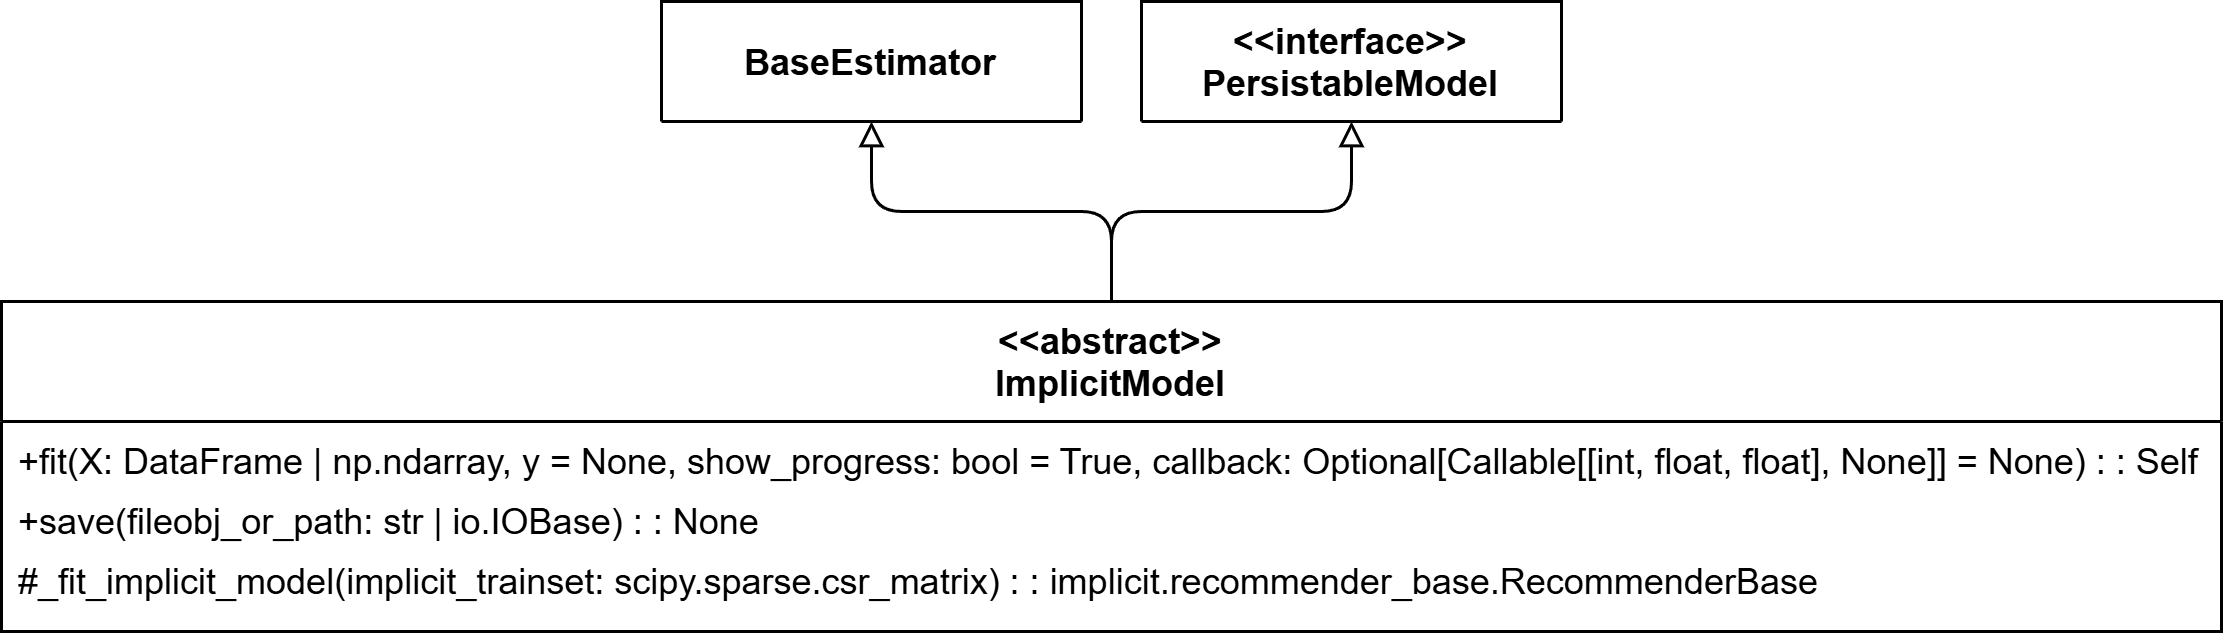
\includegraphics[scale=0.15]{figures/UML/models/implicit_model.png}
    \caption{Diagramma della classe astratta \texttt{ImplicitModel}}
\end{figure}

La classe viene estesa creando i vari adapter dei modelli:

\begin{itemize}
    \item \texttt{ALS}
    \item \texttt{BRP}
    \item \texttt{LMF}
\end{itemize}

Ogni modello riceve nel costruttore gli stessi parametri del modello originale della libreria \textit{Implicit}.

Tutti i modelli sopra elencati gestiscono feedback impliciti e quindi i valori restituiti dal metodo \textit{predict} corrispondono a \textit{rating}.

\begin{figure}[H]
    \centering
    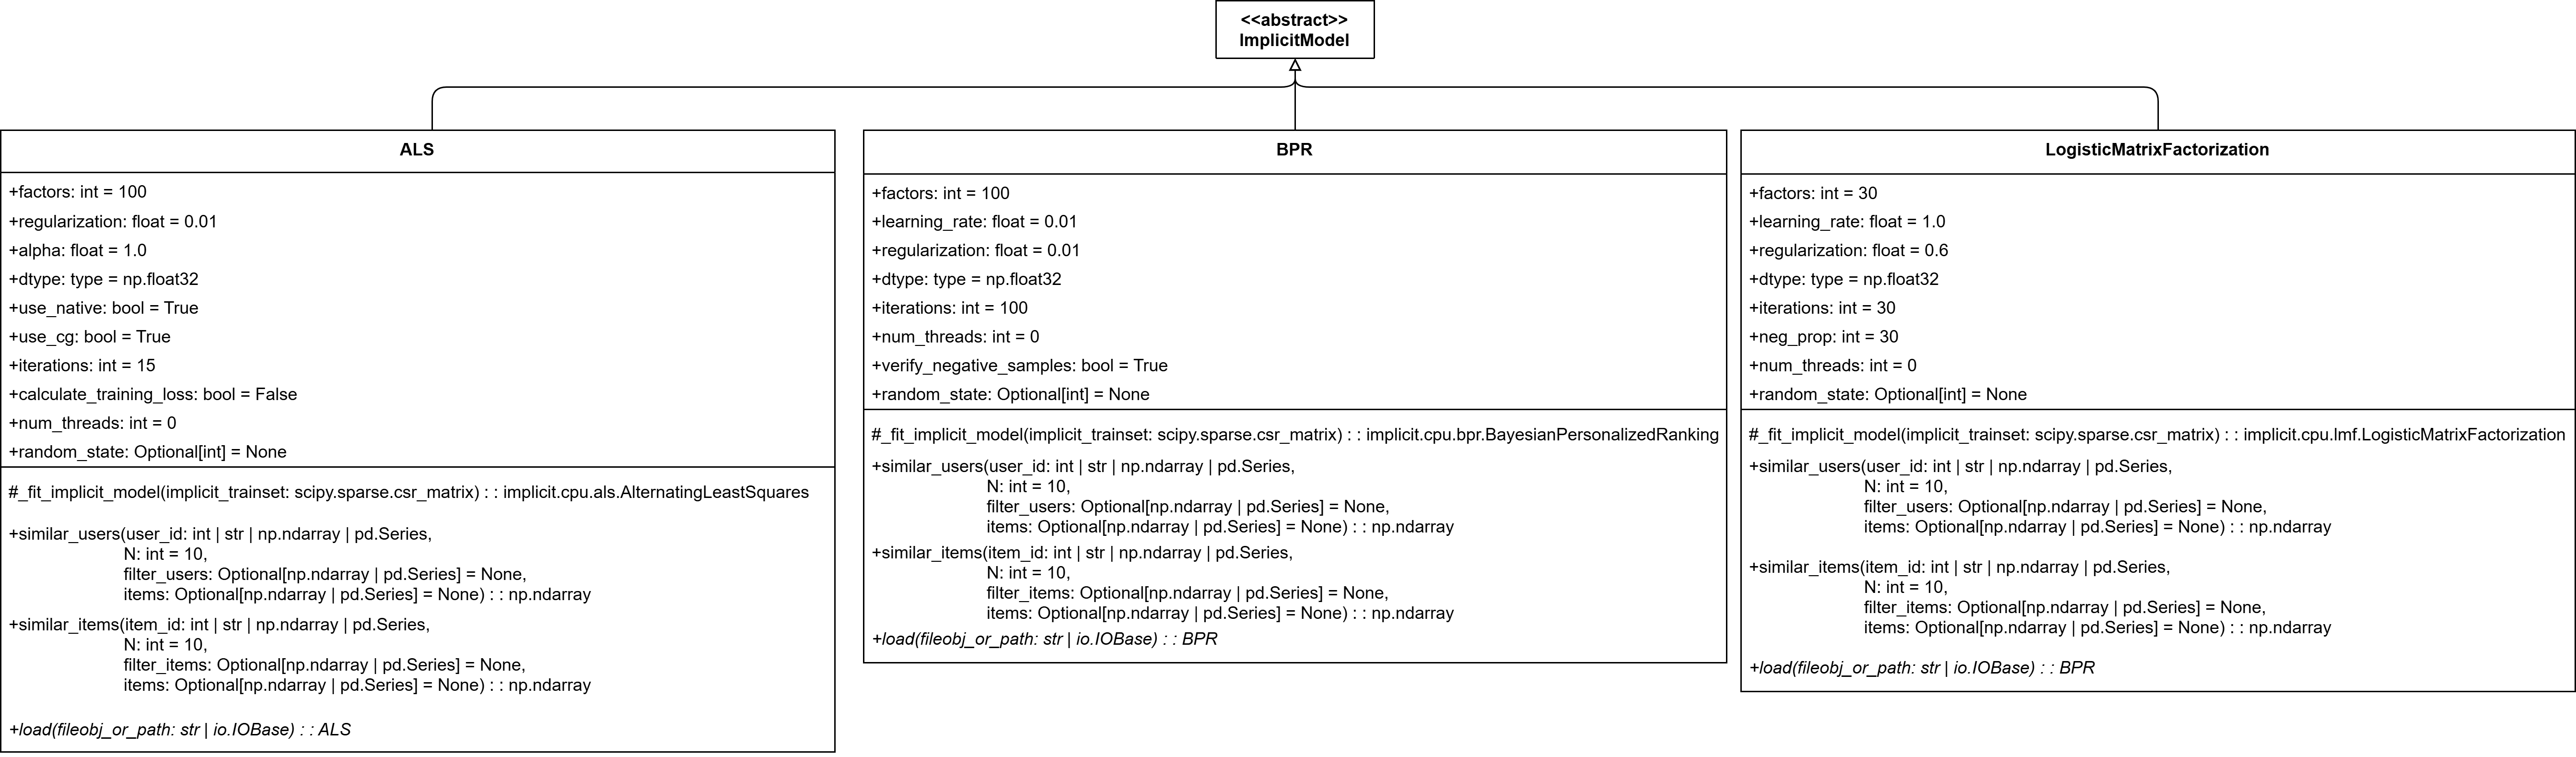
\includegraphics[angle=90, scale=0.1]{figures/UML/models/implicit_models.png}
    \caption{Diagrammi dei modelli di \textit{Implicit}}
\end{figure}

\subsubsection{Modifiche ai metodi}

Il metodo \texttt{fit} di questi modelli può riceve due parametri extra:

\begin{itemize}
    \item \texttt{show\_progress} (\texttt{bool}): indica se mostrare una barra di avanzamento durante il fitting. Il valore di default è \texttt{True}.
    \item \texttt{callback} (\texttt{Callable[[int, float, float], None]}, opzionale): funzione che viene chiamata ad ogni epoca:
    \begin{itemize}
        \item il primo parametro, di tipo \texttt{int}, corrisponde il numero corrente dell'epoca (ad esempio 1, 2, 3, \ldots)
        \item il secondo parametro, di tipo \texttt{float}, corrisponde al tempo trascorso dall'inizio dell'allenamento (in secondi, tipo \texttt{float})
        \item il terzo parametro, di tipo \texttt{float}, corrisponde alla frazione tra 0 e 1 che indica il progresso complessivo
    \end{itemize}
    Il valore di default è \texttt{None}.
\end{itemize}

\subsection{Modello LightFM}
Viene definita la classe \texttt{LightFM}, classe che estende \texttt{BaseModel}, \texttt{PersistableModel} e \texttt{SimilarityModel} e rappresenta l'\textit{Adapter} del modello \texttt{LightFM} dell'omonima libreria \texttt{LightFM}. 

Il modello gestisce feedback impliciti e quindi i valori restituiti dal metodo \textit{predict} corrispondono a \textit{score}.

\begin{figure}[H]
    \centering
    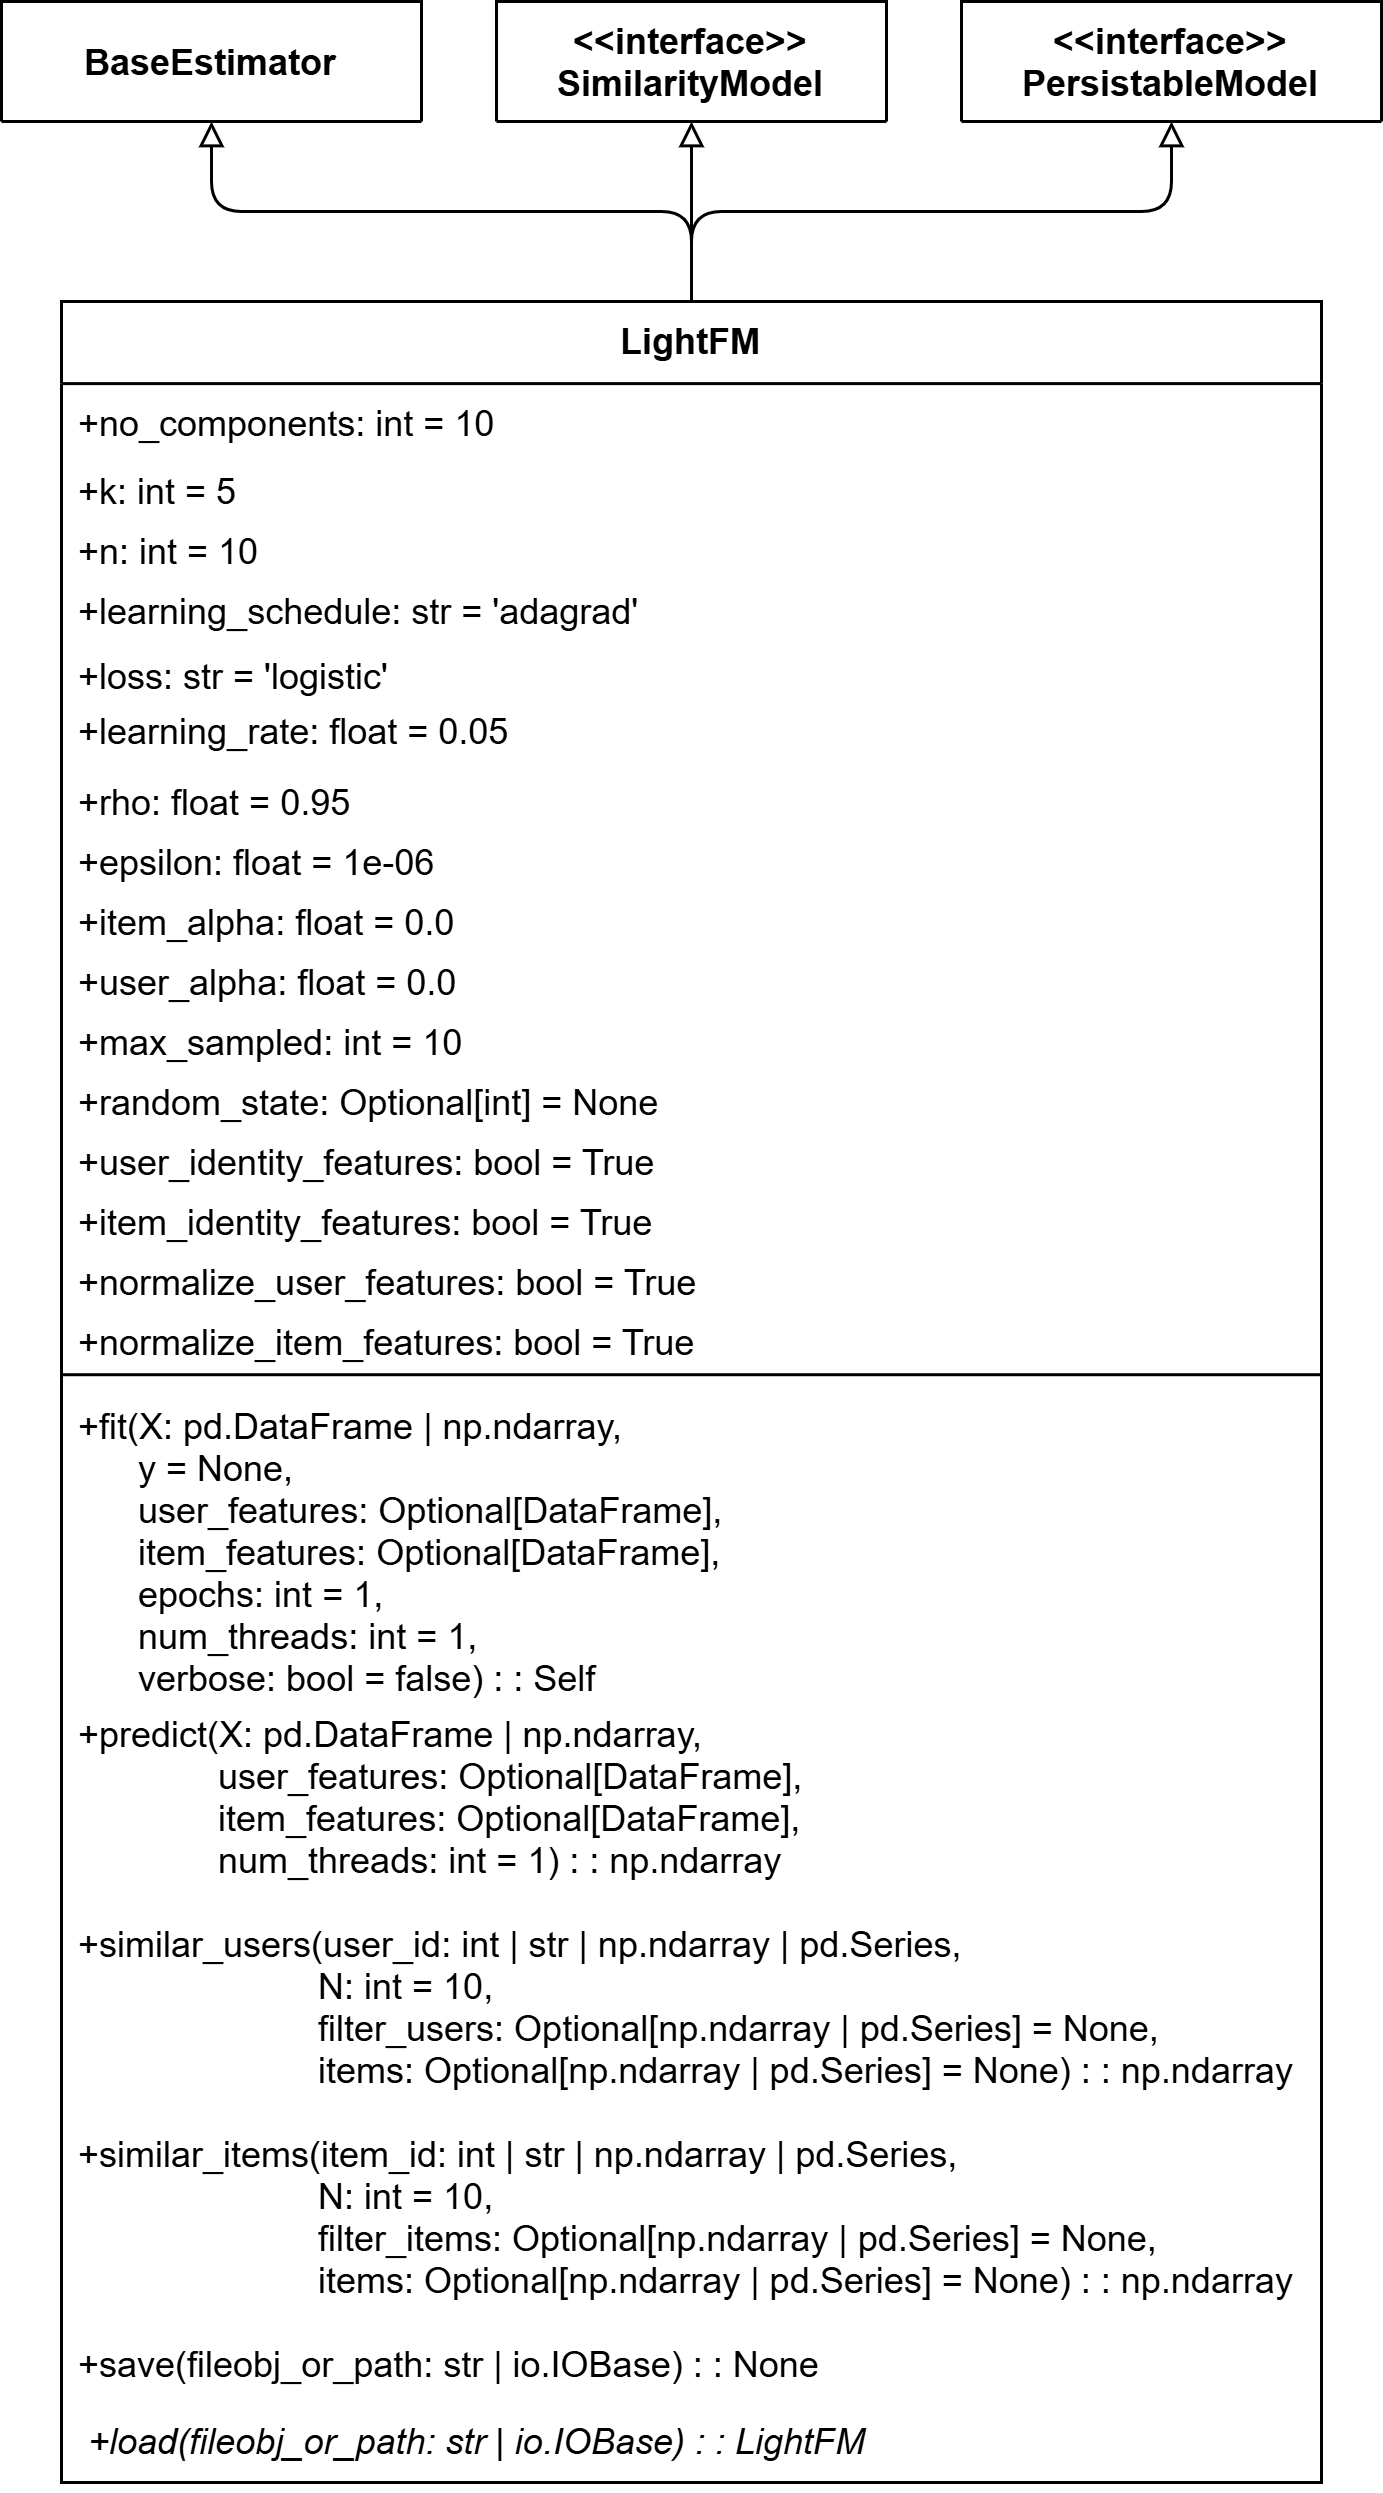
\includegraphics[scale=0.2]{figures/UML/models/light_fm.png}
    \caption{Diagrammi della classe \textit{LightFM}}
\end{figure}

\subsubsection{Costruttore}

Il costruttore riceve gli stessi parametri del modello originale della libreria \textit{LightFM} più quattro parametri extra:

\begin{itemize}
    \item \texttt{user\_identity\_features} (\texttt{bool}): crea una feature unica per ogni \textit{user} in aggiunta alle altre features. Se impostato su \texttt{True} (il valore di default), verrà allocato un vettore latente per ogni \textit{user}.  Questo è un valore predefinito ragionevole per la maggior parte delle applicazioni, ma dovrebbe essere impostato su \texttt{false} se sono disponibili pochissimi dati per ciascun \textit{user}. Per ulteriori dettagli, consultare le \textit{Note} sulla documentazione di \textit{LightFM}
    \item \texttt{item\_identity\_features} (\texttt{bool}): crea una feature unica per ogni \textit{item} in aggiunta alle altre features. Se impostato su \texttt{True} (il valore di default), verrà allocato un vettore latente per ogni \textit{item}. Questo è un valore predefinito ragionevole per la maggior parte delle applicazioni, ma dovrebbe essere impostato su \texttt{false} se sono disponibili pochissimi dati per ciascun \textit{item}. Per ulteriori dettagli, consultare le \textit{Note} sulla documentazione di \textit{LightFM}
    \item \texttt{normalize\_user\_features} (\texttt{bool}): se impostato su \texttt{True} (il valore di default), il modello utilizzerà, per l'addestramento, una versione normalizzata delle feature degli \textit{user}, garantendo che i pesi delle features sommino a 1 in ogni riga
    \item \texttt{normalize\_item\_features} (\texttt{bool}): se impostato su \texttt{True} (il valore di default), il modello utilizzerà, per l'addestramento, una versione normalizzata delle feature degli \textit{item}, garantendo che i pesi delle features sommino a 1 in ogni riga
\end{itemize}

\subsubsection{User e Item features}

\textit{LightFM} può utilizzare, sia per l'addestramento che per la predizione, informazioni aggiuntive, che corrispondono alle features di \textit{user} e di \textit{item}. 

Ciascun \textit{DataFrame} in input deve seguire la seguente struttura:
\begin{itemize}
    \item devono avere nella prima colonna tutti gli id, per \texttt{user\_id} o \texttt{item\_id}, che compaiono nel \textit{trainset}
    \item le colonne successive devono essere avere un titolo
\end{itemize}

Le stesse considerazioni valgono per le features degli \textit{user}.

Non è obbligatorio specificare entrambe le features contemporaneamente.

\begin{table}[H]
    \centering
    \begin{tabular}{|c|c|c|c|c|}
    \hline
    \textbf{item\_id} & \textbf{genre} & \textbf{pages} & \textbf{year} & \textbf{author} \\
    \hline
    B001 & Fantasy       & 432 & 2010 & Luca Ferri       \\
    B002 & Giallo        & 289 & 1998 & Martina Rossi     \\
    B003 & Sci-Fi        & 521 & 2022 & Giovanni Bianchi  \\
    B004 & Storico       & 376 & 1985 & Elena Neri        \\
    B005 & Romanzo       & 645 & 2001 & Paolo Conti       \\
    \hline
    \end{tabular}
    \caption{Esempio di \texttt{item\_features} con features su libri}
    \label{tab:book_metadata}
\end{table}

\subsubsection{Modifiche ai metodi}

Il metodo \texttt{fit} di questo modello può ricevere cinque parametri extra:

\begin{itemize}
    \item \texttt{user\_features} (\texttt{DataFrame}): matrice delle features degli \textit{user}. Il valore di default è \texttt{None}
    \item \texttt{item\_features} (\texttt{DataFrame}): matrice delle features degli \textit{item}. Il valore di default è \texttt{None}
    \item \texttt{epochs} (\texttt{int}): numero di epoche da eseguire. Il valore di default è 1
    \item \texttt{num\_threads} (\texttt{int}): numero di thread da utilizzare. Non dovrebbe essere impostato maggiore del numero di core fisici. Il valore di default è 1
    \item \texttt{verbose} (\texttt{bool}): se stampare messaggi durante l'addestramento. Se \texttt{tqdm} è installato, verrà mostrata una barra con il progresso. Il valore di default è \texttt{False}
\end{itemize}

Il metodo \texttt{predict} di questo modello può ricevere tre parametri extra:

\begin{itemize}
    \item \texttt{user\_features} (\texttt{DataFrame}): matrice delle features degli \textit{user}. Il valore di default è \texttt{None}
    \item \texttt{item\_features} (\texttt{DataFrame}): matrice delle features degli \textit{item}. Il valore di default è \texttt{None}
    \item \texttt{num\_threads} (\texttt{int}): numero di thread da utilizzare. Non dovrebbe essere impostato maggiore del numero di core fisici
\end{itemize}

\section{Model Selection}

Il modulo contiene solamente la funzione per poter eseguire lo split del 
\textit{dataset} in \textit{trainset} e \textit{testset}, chiamata \texttt{train\_test\_split\_with\_coverage}. 

La funzione riceve in ingresso un \textit{DataFrame} o un \textit{NumPy array} che deve rispettare il formato standard definito sui dati che utilizzano i modelli~\ref{model_fit_data}. 

Lo \textit{split} viene effettuato in modo che nel \textit{trainset} ci sia almeno un'interazione per ogni \textit{user} e ogni \textit{item} in modo che, durante la \textit{prediction}, sia possibile generare un risultato per qualunque \textit{user}/\textit{item} presente durante la fase di \textit{training}. Non ci sono invece sicurezze sul fatto che nel \textit{testset} ci sia, per ogni \textit{user}/\textit{item}, almeno un'interazione. Questo potrebbe portare ad un caso particolare di \textit{cold-start} nel \textit{testset}.


\section{Model Evaluation}
Il modulo comprende l'insieme delle funzioni per calcolare le prestazioni dei modelli addestrati.

Per i modelli che gestiscono feedback espliciti sono presenti i seguenti algoritmi:

\begin{itemize}
    \item Root Mean Squared Error (RMSE) con la funzione \texttt{rmse}
    \item Mean Absolute Error (MAE) con la funzione \texttt{mae}
\end{itemize}

mentre per quelli che gestiscono feedback impliciti:

\begin{itemize}
    \item Precision@K con la funzione \texttt{precision\_at\_k}
    \item Recall@K con la funzione \texttt{recall\_at\_k}
    \item F1@K con la funzione \texttt{f1\_at\_k}
    \item Hit@K con la funzione \texttt{hit\_at\_k}
    \item Area Under the ROC Curve (AUC) con la funzione \texttt{auc}
    \item Normalized Discounted Cumulative Gain (NDCG) con la funzione \texttt{ndcg}
\end{itemize}

\section{Utils}

Il modulo \texttt{utils} raccoglie un insieme di funzioni ausiliarie progettate per supportare attività comuni nella fase di preparazione dei dati e predizione nei modelli di raccomandazione. Le funzioni sono pensate per essere modulari, riutilizzabili e indipendenti dalla specifica implementazione del modello.

\begin{itemize}
    \item \texttt{check\_model\_inputs}: funzione di validazione degli input forniti a un modello. Controlla che tutte le colonne richieste siano presenti, che i dati siano nel formato standard (vedere~\ref{model_fit_data} e~\ref{model_predict_data}) e che rispettino le specifiche attese dal modello. Può essere inclusa nei metodi \texttt{fit} e \texttt{predict} dei modelli che accettano i dati nel formato standard

    \item \texttt{generate\_user\_item\_pairs}: prende in input una matrice (in formato \textit{DataFrame} o \textit{NumPy array}) che contiene almeno due colonne: la prima con gli \texttt{user\_id} e la seconda con gli \texttt{item\_id}. Le eventuali colonne aggiuntive vengono ignorate. La funzione genera un \textit{DataFrame} contenente tutte le coppie possibili (\texttt{user\_id}, \texttt{item\_id}) ottenute dal prodotto cartesiano tra gli \textit{user} e gli \textit{item} presenti nei dati forniti. Questo serve affinché i modelli possano calcolare, tramite il metodo \texttt{predict}, il \textit{ranking} di tutti gli \textit{item} per ciascuno \textit{user}
    \begin{table}[H]
        \centering
        \begin{minipage}{\textwidth}
            \centering
            \textbf{Input (user\_id, item\_id)}\\[0.5em]
            \begin{tabular}{|c|c|c|}
            \hline
            \textbf{user\_id} & \textbf{item\_id} & \textbf{timestamp} \\
            \hline
            1 & 10 & 2025-01-01 \\
            2 & 11 & 2025-01-02 \\
            3 & 12 & 2025-01-03 \\
            \hline
            \end{tabular}
        \end{minipage}

        \vspace{1em} % Spazio verticale tra le tabelle

        \begin{minipage}{\textwidth}
            \centering
            \textbf{Output (prodotto cartesiano)}\\[0.5em]
            \begin{tabular}{|c|c|}
            \hline
            \textbf{user\_id} & \textbf{item\_id} \\
            \hline
            1 & 10 \\
            1 & 11 \\
            1 & 12 \\
            2 & 10 \\
            2 & 11 \\
            2 & 12 \\
            3 & 10 \\
            3 & 11 \\
            3 & 12 \\
            \hline
            \end{tabular}
        \end{minipage}
        \caption{Esempio di input e output per \texttt{generate\_user\_item\_pairs}}
    \end{table}
\end{itemize}


\section{Visualization}
Il modulo comprende l'insieme delle funzioni di supporto dedicate all'analisi esplorativa e alla visualizzazione di dati in formato \textit{DataFrame}. In particolare, fornisce strumenti per rappresentare graficamente la distribuzione di variabili continue e categoriali tramite istogrammi, curve di densità e grafici a barre, facilitando la comprensione della frequenza e della percentuale dei valori presenti. Inoltre, include una funzione principale, \texttt{describe}, che, data una struttura dati tabellare, consente di visualizzare in modo personalizzato le distribuzioni di colonne categoriali e continue, supportando anche colonne con valori multipli separati da un delimitatore.

Questo modulo è stato pensato per poter visualizzare ed analizzare le distribuzioni di eventuali \textit{rating} e features di \textit{user} e \textit{item}.

\begin{itemize}

  \item \texttt{plot\_hist}: è una funzione per visualizzare la distribuzione di una variabile continua sotto forma di istogramma. Utilizza la libreria \texttt{seaborn} per generare il grafico, con la possibilità di specificare il numero di intervalli (\texttt{bins}) oppure lasciare che vengano determinati automaticamente. È utile per esplorare la frequenza dei valori e la forma generale della distribuzione (simmetrica, asimmetrica, ecc.)

  \item \texttt{plot\_continuous\_distribution}: genera una stima della densità di probabilità di una variabile continua tramite il metodo \texttt{kdeplot} (Kernel Density Estimation). Questo tipo di grafico è utile per comprendere la forma teorica della distribuzione, in modo più fluido e continuo rispetto all'istogramma, mettendo in evidenza eventuali picchi, code o multi-modalità nei dati.

  \item \texttt{plot\_categorical\_distribution}: visualizza la distribuzione di una variabile categorica. Può opzionalmente suddividere valori multipli contenuti in una singola cella (e.g. stringhe separate da virgole) tramite \textit{split}. I valori vengono contati e mostrati in un grafico a barre orizzontali, con etichette descrittive che indicano il numero assoluto e la percentuale relativa di ciascuna categoria. È particolarmente utile per analizzare la frequenza delle classi o delle etichette presenti nei dati

  \item \texttt{describe}: è una funzione riassuntiva che combina più strumenti di esplorazione visiva per un'intero \textit{DataFrame}. Permette di specificare quali colonne siano categoriche, continue o da visualizzare tramite istogrammi, e genera automaticamente i grafici appropriati per ciascuna tipologia. È pensata per offrire un'esplorazione iniziale rapida dei dati, facilitando l'analisi preliminare tramite visualizzazioni mirate. Può anche stampare il contenuto del \textit{DataFrame} se richiesto

\end{itemize}
% \chapter{Implementazione}

\section{Ambiente di Sviluppo e Gestione delle Dipendenze}

Lo sviluppo della libreria è stato effettuato utilizzando \textit{Python} 3.11, con le seguenti versioni delle principali librerie di raccomandazione:

\begin{itemize}
  \item \textit{Surprise} 1.1.4
  \item \textit{Implicit} 0.7.2
  \item \textit{LightFM} 1.17
\end{itemize}

A causa di incompatibilità tra \textit{Surprise} e le versioni più recenti di \textit{NumPy}, è stato necessario utilizzare la versione 1.24.4 di \textit{NumPy}. Tale scelta non ha comportato problemi di compatibilità con le altre librerie utilizzate.

Per la gestione dei pacchetti e delle dipendenze è stato utilizzato \textit{uv}, un gestore di pacchetti Python di nuova generazione sviluppato da \textit{Astral} (gli stessi creatori di \textit{ruff}). Scritto in \textit{Rust}, \textit{uv} si distingue per le sue elevate prestazioni, risultando fino a 10--100 volte più veloce rispetto a \textit{pip}. Questo è particolarmente importante in contesti in cui la libreria viene installata frequentemente, come durante il rilascio in ambienti cloud mediante l'utilizzo di \textit{CI/CD}.

Oltre a offrire un'interfaccia compatibile con \textit{pip}, \textit{uv} integra diverse funzionalità avanzate, tra cui:

\begin{itemize}
  \item creazione e gestione di ambienti virtuali (\texttt{uv venv});
  \item risoluzione e sincronizzazione delle dipendenze con lockfile universali (\texttt{uv pip compile}, \texttt{uv pip sync})
  \item installazione di pacchetti da file standard come \texttt{requirements.txt} e \\ \texttt{pyproject.toml}
  \item supporto per installazioni da repository \textit{Git}, URL e pacchetti locali
\end{itemize}

\section{Implementazione dei modelli}

\subsection{Surprise}

La classe astratta \texttt{SurpriseModel} implementa internamente la logica per la gestione del \textit{dataset} e il salvataggio dei modelli. 

Alcune considerazioni sull'implementazione:

\begin{itemize}
    \item per l'addestramento e la previsione viene utilizzata la struttura dati \\ \texttt{surprise.dataset.Dataset}, creata con la chiamata al metodo statico \\ \texttt{load\_from\_df} della classe stessa utilizzando direttamente dai dati passati tramite le funzioni \texttt{fit} e \texttt{predict}. Il valore del parametro \texttt{rating\_scale} dell'oggetto \texttt{surprise.reader.Reader}, che viene utilizzato per la creazione dell'oggetto \texttt{Dataset}, viene impostato come \texttt{(rating\_column.min, \\ rating\_column.max)}. Se non sono presenti i \textit{rating} nel \textit{trainset}, il valore di default viene impostato a \texttt{(0, 1)}
    \item per il salvataggio, all'interno del metodo \texttt{save} viene utilizzato il metodo \texttt{pickle.dump} per serializzare il modello
    \item il metodo statico \texttt{load} che implementa ogni sottoclasse utilizza invece il metodo \texttt{pickle.load} per deserializzare il file salvato e ricostruire il modello
\end{itemize}

\subsection{Implicit}

La classe astratta \texttt{ImplicitModel} implementa internamente la logica per la gestione del \textit{dataset} e il salvataggio dei modelli. 

Alcune considerazioni sull'implementazione:

\begin{itemize}
    \item per l'addestramento e la previsione i dati vengono convertiti da \textit{DataFrame} a \textit{csr\_matrix}. Per prima cosa si crea e si salva una versione \textit{encoded}, tramite l'oggetto \texttt{sklearn.preprocessing.LabelEncoder} dei vari id. Viene creata una matrice in formato \textit{COO} utilizzando la funzione \texttt{sparse.coo\_matrix} della libreria \textit{Scipy}. In questo passaggio, se nel \textit{trainset} non è presente la terza colonna contenente i pesi dell'interazione, viene aggiunta una colonna \textit{placeholder} tutta con valore 1. Infine la matrice viene convertita in formato \textit{CSR} tramite la funzione \texttt{coo\_matrix.tocsr()} 
    \item per il salvataggio, all'interno del metodo \texttt{save} viene utilizzato il metodo \texttt{save} già presente nei modelli di \textit{Implicit} che salva il modello usando il formato \textit{.npz} di \textit{NumPy}
    \item il metodo statico \texttt{load} che implementa ogni sottoclasse utilizza invece il metodo \texttt{load} che ogni modello \textit{Implicit} già implementa
\end{itemize}

\subsection{LightFM}

La classe \texttt{LightFM} implementa internamente la logica per la gestione del \textit{dataset} e il salvataggio dei modelli. 

Alcune considerazioni sull'implementazione:

\begin{itemize}
    \item per l'addestramento e la previsione i dati vengono convertiti da \textit{DataFrame} a \textit{coo\_matrix}. Per prima cosa si crea e si salva una versione \textit{encoded}, tramite l'oggetto \texttt{sklearn.preprocessing.LabelEncoder} dei vari id. Viene creata una matrice in formato \textit{COO} utilizzando il metodo \texttt{build\_interactions} dell'oggetto \texttt{lightfm.data.Dataset}. In questo passaggio, se nel \textit{trainset} non è presente la terza colonna contenente i pesi dell'interazione, viene aggiunta una colonna \textit{placeholder} tutta con valore 1. 
    \item se sono presenti delle features vengono chiamati i metodi \\ \texttt{build\_item\_features} e \texttt{build\_user\_features} dell'oggetto \\ \texttt{lightfm.data.Dataset} per creare le features degli \textit{item} e degli \textit{user}
    \item per il salvataggio, all'interno del metodo \texttt{save} viene utilizzato il metodo \texttt{pickle.dump} per serializzare il modello
    \item il metodo statico \texttt{load} utilizza invece il metodo \texttt{pickle.load} per deserializzare il file salvato e ricostruire il modello
\end{itemize}

\section{Parametri appresi}

Affinché qualunque istanza di una classe che estenda \texttt{BaseModel} si possa considerare addestrata deve esporre almeno un campo il cui nome termini con "\_". Di seguito vengono definiti quali campi vengono esposti da ciascun \textit{transformer} e ciascun modello. Alcuni \textit{transformers}, data la loro natura \textit{stateless}, non apprendono nulla e, di conseguenza, non espongono nessun nuovo campo.

Per i \textit{transformers}:

\begin{itemize}
    \item \texttt{LabelEncoder}: \texttt{classes\_}, un array che contenente un'etichetta per ciascuna classe
    \item \texttt{Bin}: \texttt{bin\_edges\_} con intervalli dei bin appresi
    \item \texttt{StandardScaler}:
    \begin{itemize}
        \item \texttt{scale\_} : scala relativa per ogni feature dei dati per ottenere media zero e varianza unitaria. Generalmente calcolata come \texttt{np.sqrt(var\_)}. Se la varianza è zero, non si può ottenere varianza unitaria e il fattore di scala è 1. È \texttt{None} se \texttt{with\_std=False}
        \item \texttt{mean\_} : valore medio per ogni feature nel set di addestramento. È \texttt{None} se \texttt{with\_mean=False} e \texttt{with\_std=False}
        \item \texttt{var\_} : varianza per ogni feature nel set di addestramento, usata per calcolare \texttt{scale\_}. È \texttt{None} se \texttt{with\_mean=False} e \texttt{with\_std=False}
        \item \texttt{n\_features\_in\_} : numero di feature viste durante il \texttt{fit}
        \item \texttt{feature\_names\_in\_} : nomi delle feature viste durante il \texttt{fit}, definiti solo se \texttt{X} ha nomi di feature tutti stringa
        \item \texttt{n\_samples\_seen\_} : numero di campioni processati dal modello per ogni feature. Se non ci sono dati mancanti è un intero, altrimenti un array di interi. Se si usano pesi campionari è un float o un array di float che somma i pesi finora visti. Viene azzerato ad ogni nuova chiamata a \texttt{fit}, ma incrementa nelle chiamate a \texttt{partial\_fit}
        \item \texttt{inverse\_transformers\_} : dizionario che contiene le funzioni di trasformazione inversa apprese, usato per applicare trasformazioni inverse specifiche su feature o gruppi di feature
    \end{itemize}
    \item \texttt{Normalizer}:
    \begin{itemize}
        \item \texttt{n\_features\_in\_} : numero di feature viste durante il \texttt{fit}
        \item \texttt{feature\_names\_in\_} : nomi delle feature viste durante il \texttt{fit}, definiti solo se \texttt{X} ha nomi delle feature tutti di tipo stringa
        \item \texttt{transformers\_} : dizionario che contiene le funzioni di trasformazione apprese, usato per applicare trasformazioni specifiche su feature o gruppi di feature
    \end{itemize}
    \item \texttt{OneHotEncode}: 
    \begin{itemize}
        \item \texttt{categories\_list\_} : liste di array contenenti le categorie di ogni feature determinate durante il \texttt{fit}, ordinate come le feature in \texttt{X} e corrispondenti all'output della trasformazione. Include la categoria specificata in \texttt{drop}, se presente
        \item \texttt{drop\_idx\_} : array di dimensione \texttt{(n\_features,)} con l'indice della categoria da scartare per ogni feature. Se non c'è nessuna categoria da scartare, il valore è \texttt{None}. Può essere \texttt{None} anche se tutte le feature sono mantenute. Se sono abilitate categorie infrequenti tramite \texttt{min\_frequency} o \texttt{max\_categories}, e l'indice corrisponde a una categoria infrequente, tutta la categoria infrequente viene scartata
        \item \texttt{infrequent\_categories\_list\_} : array contenente le categorie infrequenti per ogni feature
        \item \texttt{n\_features\_in\_} : numero di feature viste durante il \texttt{fit}
        \item \texttt{feature\_names\_in\_} : nomi delle feature viste durante il \texttt{fit}, se disponibili
        \item \texttt{feature\_name\_combiner} : funzione con \textit{signature} \\ \texttt{def callable(input\_feature, category)} che restituisce una stringa usata per creare i nomi delle feature da restituire con \\ \texttt{get\_feature\_names\_out}
    \end{itemize}
    \item \texttt{MinMaxScaler}:
    \begin{itemize}
        \item \texttt{min\_} : aggiustamento per ogni feature del valore minimo. Equivale a \\ \texttt{min - X.min(axis=0) * scale\_}
        \item \texttt{scale\_} : scala relativa per ogni feature dei dati. Equivale a \\ \texttt{(max - min) / (X.max(axis=0) - X.min(axis=0))}
        \item \texttt{data\_min\_} : minimo osservato per ogni feature nei dati
        \item \texttt{data\_max\_} : massimo osservato per ogni feature nei dati
        \item \texttt{data\_range\_} : intervallo (massimo - minimo) osservato per ogni feature nei dati
        \item \texttt{n\_features\_in\_} : numero di feature viste durante il \texttt{fit}
        \item \texttt{n\_samples\_seen\_} : numero di campioni elaborati dall'estimatore
        \item \texttt{feature\_names\_in\_} : nomi delle feature viste durante il \texttt{fit}, se disponibili
        \item \texttt{transformers\_} : dizionario che contiene le funzioni di trasformazione apprese, usato per applicare trasformazioni specifiche su feature o gruppi di feature
        \item \texttt{inverse\_transformers\_} : dizionario che contiene le funzioni di trasformazione inversa apprese, usato per applicare trasformazioni inverse specifiche su feature o gruppi di feature
    \end{itemize}
    \item \texttt{BinDensity} e \texttt{BinCumulative}:
    \begin{itemize}
        \item \texttt{feature\_values\_} : insieme dei valori presenti nella colonna del feature durante il \textit{fit}
        \item \texttt{excluded\_features\_} : sottoinsieme di valori identificati per essere esclusi (definiti dalla logica di split)
        \item \texttt{grouped\_features\_} : sottoinsieme di valori raggruppati (definiti dalla logica di split)
    \end{itemize}
\end{itemize}

Tutti i modelli apprendono ed espongono come attributi anche \texttt{user\_ids\_} e \texttt{item\_ids\_} e \texttt{train\_user\_item\_pairs\_}, che corrispondono rispettivamente a due liste ordinate degli id di \texttt{user} e \texttt{item} e ad un set di coppie (\textit{user\_id}, \textit{item\_id}) viste durante l'addestramento. Questi valori vengono anche utilizzati dalle funzioni di evaluation implicite, quindi i modelli che intendono utilizzare le implementazioni proposte devono esporre questi attributi.

Gli altri attributi sono:

\begin{itemize}
    \item \texttt{ALS}, \texttt{BPR} e \texttt{LMF}:
    \begin{itemize}
        \item \texttt{item\_factors\_} : dizionario contenente, per ogni \textit{item} id, i fattori latenti appresi
        \item \texttt{user\_factors\_} : dizionario contenente, per ogni \textit{user} id, i fattori latenti appresi
    \end{itemize}
    \item \texttt{SVD}, \texttt{SVDpp} e \texttt{NMF}:
    \begin{itemize}
        \item \texttt{pu\_} : dizionario che contiene, per ogni \textit{user} id, i fattori latenti appresi. Ogni valore ha dimensione \textit{num. factors}
        \item \texttt{qi\_} : dizionario che contiene, per ogni \textit{item} id, i fattori latenti appresi. Ogni valore ha dimensione \textit{num. factors}
        \item \texttt{yj\_} (solo \texttt{SVDpp}) : dizionario che contiene, per ogni \textit{item} id, i fattori impliciti appresi. Ogni valore ha dimensione \textit{num. factors}. Serve a modellare il comportamento implicito degli \textit{user}
        \item \texttt{bu\_} : dizionario che contiene, per ogni \textit{user} id, il bias di quello \textit{user}
        \item \texttt{bi\_} : dizionario che contiene, per ogni \textit{item} id, il bias di quell'\textit{item}
    \end{itemize}
    \item \texttt{KNNBaseline}: 
    \begin{itemize}
        \item \texttt{xr\_} : dizionario che contiene, per ogni \textit{user}/\textit{item} id, i vettori di riferimento per i \textit{user}/\textit{item} (e.g. vettori dei \textit{user} nel k-NN user-based)
        \item \texttt{yr\_} : dizionario complementare a \texttt{xr\_}
        \item \texttt{n\_xv\_} : numero di elementi nel dataset corrispondenti a \texttt{xr\_} (e.g. numero di \textit{user})
        \item \texttt{n\_y\_} : numero di elementi nel dataset corrispondenti a \texttt{yr\_} (e.g. numero di \textit{item})
        \item \texttt{bx\_} : dizionario che contiene, per ogni \textit{user}/\textit{item} id, il bias dell'elemento corrispondente in \texttt{xr\_} (e.g. bias dei \textit{user})
        \item \texttt{by\_} : dizionario complementare a \texttt{bx\_}
        \item \texttt{k\_} : numero di vicini usati nel \textit{KNN}
    \end{itemize}

    \item \texttt{SlopeOne}:
    \begin{itemize}
        \item \texttt{freq\_} : dizionario delle frequenze di co-valutazione tra coppie di \textit{item}. \texttt{freq\_[i][j]} indica il numero di \textit{user} che hanno valutato sia l'\textit{item} \texttt{i} che l'\textit{item} \texttt{j}.
        \item \texttt{dev\_} : dizionario delle differenze medie (deviazioni) tra coppie di \textit{item}. \texttt{dev\_[i][j]} indica la differenza media dei \textit{rating} tra l'\textit{item} \texttt{i} e l'\textit{item} \texttt{j}, calcolata sui soli \textit{user} che hanno valutato entrambi

    \end{itemize}
    \item \texttt{CoCluster}:
    \begin{itemize}
        \item \texttt{avg\_cltr\_i\_} : media dei cluster per \textit{item}
        \item \texttt{avg\_cltr\_u\_} : media dei cluster per \textit{user}
        \item \texttt{avg\_cocltr\_} : media dei \textit{co-cluster}
        \item \texttt{bi\_} : dizionario che contiene, per ogni \textit{item} id, il bias di quell'\textit{item}
        \item \texttt{bu\_} : dizionario che contiene, per ogni \textit{user} id, il bias di quello \textit{user}
        \item \texttt{bsl\_options\_} : opzioni per il calcolo delle baseline
        \item \texttt{cltr\_i\_} : cluster degli \textit{item}
        \item \texttt{cltr\_u\_} : cluster degli \textit{user}
        \item \texttt{item\_mean\_} : dizionario che contiene, per ogni \textit{item} id, la media delle valutazioni di quell'\textit{item}
        \item \texttt{n\_cltr\_i\_} : numero di cluster \textit{item}
        \item \texttt{n\_cltr\_u\_} : numero di cluster \textit{user}
        \item \texttt{n\_epochs\_} : numero di epoche di addestramento
        \item \texttt{user\_mean\_} : dizionario che contiene, per ogni \textit{user} id, la media delle valutazioni di quello \textit{user}
    \end{itemize}
    \item \texttt{LightFM}:
    \begin{itemize}
        \item \texttt{user\_biases\_} : dizionario che contiene, per ogni \textit{user} id, il bias di quello \textit{user}
        \item \texttt{user\_embeddings\_} : dizionario che contiene, per ogni \textit{user} id, la rappresentazione latente di quello \textit{user}. Ogni valore ha dimensione \textit{num. components}
        \item \texttt{item\_biases\_} : dizionario che contiene, per ogni \textit{item} id, il bias di quell'\textit{item}
        \item \texttt{item\_embeddings\_} : dizionario che contiene, per ogni \textit{item} id, la rappresentazione latente di quell'\textit{item}. Ogni valore ha dimensione \textit{num. components}
    \end{itemize}


\begin{lstlisting}[caption=Esempio di utilizzo dei parametri appresi]
light_fm = LightFM(no_components=30)
# the use of light_fm.user_embeddings_ before fit raises NotFittedError because models is not fitted yet
light_fm.fit(train, epochs=20)
print(light_fm.user_embeddings_) # shows a matrix of shape (num_users, 30)
\end{lstlisting}

\end{itemize}

\section{Calcolo della similarità item-item e user-user}

Per ciascun modello che estende l'interfaccia \texttt{SimilarityModel} viene specificato il tipo di similarità utilizzata e come viene calcolata.

\begin{itemize}
    \item i modelli \texttt{SVD}, \texttt{SVDpp} e \texttt{NMF} utilizzano la similarità coseno, calcolata tramite la funzione \texttt{cosine\_similarity} di \textit{Scikit-learn}. La matrice di similarità viene calcolata utilizzando \texttt{pu\_} degli \textit{user} o \texttt{qi\_} degli \textit{item} appresi dal modello.
    
    Per \texttt{SVDpp} viene utilizzata anche la rappresentazione implicita degli \textit{item} \texttt{yj\_} per calcolare la rappresentazione dell'\textit{user}:

    \[\vec{p}_u^{\text{ SVD++}} = \vec{p}_u + \frac{1}{|N(u)|} \sum_{j \in N(u)} \vec{y}_j\]

    dove $N(u)$ è l'insieme degli \textit{item} valutati dall'utente

    \item \texttt{KNNBaseline} utilizza la similarità specificata nel parametro \texttt{sim\_options} che può essere similarità coseno, \textit{Pearson} con o senza baseline e \textit{MSD}. Il calcolo viene applicato sui vettori di \texttt{xr\_} e \texttt{yr\_} appresi dal modello. La similarità coseno viene calcolata tramite la funzione \texttt{cosine\_similarity} di \textit{Scikit-learn}, mentre la similarità \textit{Pearson} e \textit{MSD} vengono calcolate tramite le funzioni \texttt{surprise.similarities.pearson} o \\ \texttt{surprise.similarities.pearson\_baseline} e \\ \texttt{surprise.similarities.msd} della libreria \textit{Surprise}
    \item \texttt{LightFM} utilizza la similarità coseno tra le rappresentazioni latenti degli \textit{item} e degli \textit{user} presenti in \texttt{item\_embeddings\_} e \texttt{user\_embeddings\_}. Il calcolo viene effettuato tramite la funzione \texttt{cosine\_similarity} di \textit{Scikit-learn}
    \item \texttt{ALS}, \texttt{BPR} e \texttt{LMF} implementano la similarità tra \textit{item} e \textit{user} utilizzando i metodi \texttt{similar\_user} e \texttt{similar\_item} delle classi base della libreria \textit{Implicit} che internamente utilizzano similarità coseno o \textit{dot product}
\end{itemize}

\section{Scelta dei grafici per la Data Visualization}

Per i grafici generati dalle funzioni presenti nel modulo di \texttt{visualization} si è deciso di utilizzare la libreria \textit{Seaborn}, in quanto offre uno stile grafico gradevole di default, un'integrazione diretta con i \textit{DataFrame} e la possibilità di creare grafici complessi e statisticamente informativi con poche righe di codice.

Un esempio di quello che si può ottenere analizzando \textit{dataset} e features:

\begin{figure}[H]
    \centering

    \begin{subfigure}[b]{0.60\textwidth}
        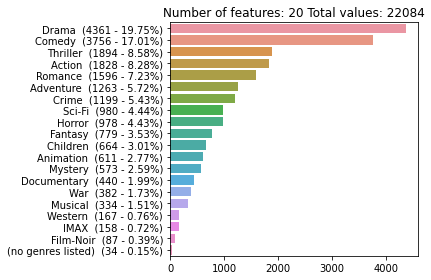
\includegraphics[width=\textwidth]{figures/visualization/output.png}
    \end{subfigure}
    \hfill
    \begin{subfigure}[b]{0.49\textwidth}
        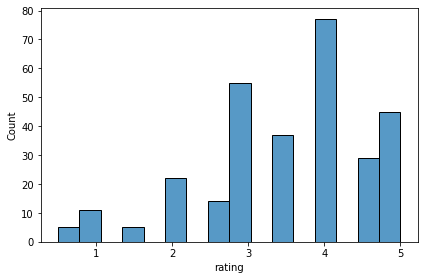
\includegraphics[width=\textwidth]{figures/visualization/output2.png}
    \end{subfigure}
    \hfill
    \begin{subfigure}[b]{0.49\textwidth}
        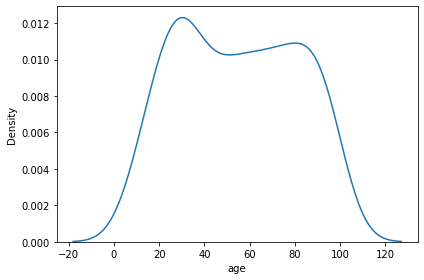
\includegraphics[width=\textwidth]{figures/visualization/output3.png}
    \end{subfigure}

    \caption{Visualizzazione esplorativa dei dati. In alto: distribuzione dei generi cinematografici presenti nel dataset, originariamente uniti in gruppi contenti più generi e uniti dal carattere "|". In basso a sinistra: istogramma delle valutazioni assegnate dagli \textit{user}. In basso a destra: distribuzione delle età degli \textit{user}.}
\end{figure}

\section{Model Selection}

la funzione \texttt{train\_test\_split\_with\_coverage} riceve in ingresso un \textit{DataFrame} o un \textit{NumPy array} contenente le interazioni tra \textit{user} e \textit{item}, e una percentuale (o numero assoluto) che definisce la dimensione del \textit{testset}. L'obiettivo è selezionare casualmente una porzione di interazioni da rimuovere dal \textit{dataset} iniziale, ma solo se la loro rimozione non comporta la perdita completa di informazioni su alcun \textit{user} o \textit{item} nel \textit{trainset}.

L'algoritmo procede nel modo seguente:
\begin{enumerate}
    \item conta per ciascun \textit{user} e ciascun \textit{item} il numero di interazioni
    \item mescola il \textit{dataset} in modo riproducibile (tramite \texttt{random\_state})
    \item itera sul \textit{dataset} cercando di rimuovere righe che non siano le uniche a coinvolgere uno specifico \textit{user} o \textit{item}
    \item appena raggiunta la dimensione desiderata del \textit{testset}, il processo si arresta
    \item in caso non fosse possibile possibile generare un \textit{testset} della dimensione specificata viene sollevata un'eccezione
\end{enumerate}

Questo approccio garantisce che il \textit{trainset} contenga almeno un'interazione per ogni \textit{user} e ogni \textit{item}, evitando problemi di id mai visti durante la predizione.

La funzione \texttt{random\_train\_test\_split} è ispirata alla omonima funzione della libreria \textit{Scikit-learn}, ma i tipo di dati in input e in output è un \textit{DataFrame}.

\section{Evaluation}

Le funzioni all'interno del modulo di \textit{evaluation} sono state pensate per essere utilizzate all'interno dell'oggetto \texttt{GridSearchCV} di \textit{Scikit-learn}, che permette di effettuare la ricerca dei migliori iperparametri per un modello tramite \textit{cross-validation}.

L'oggetto riceve come parametro \texttt{scoring} una funzione che calcola la metrica di valutazione desiderata. Per i modelli espliciti, le metriche di valutazione \textit{RMSE} e \textit{MAE} sono già presenti all'interno di \textit{Scikit-learn} e non necessitano di adattamenti. 

Tuttavia, per i modelli impliciti, è necessario definire una funzione di valutazione personalizzata che calcoli la metrica desiderata, dato che i modelli non restituiscono direttamente i valori previsti, ma piuttosto degli \textit{score}. Tutte le metriche sono calcolate considerando il \textit{ranking} costruito utilizzando gli \textit{score} di tutti i possibili \textit{item} per tutti i possibili \textit{user}.

Le funzioni di scoring passate al parametro \texttt{scoring} di \textit{Scikit-learn} ricevono in ingresso il modello, \texttt{X}, che corrisponde al \textit{DataFrame} o \textit{NumPy array} di \textit{testset}, e \texttt{y}, non utilizzato ma specificato per compatibilità con la libreria. Il problema è che i modelli hanno bisogno di tutti gli id di \textit{user} e \textit{item} in modo da poter calcolare lo score per tutte le possibili coppie (\textit{user\_id}, \textit{item\_id}); inoltre, alcune di esse erano già presenti nel \textit{trainset} e non devono essere considerate nuovamente. Queste informazioni sono contenute negli attributi \texttt{user\_ids\_}, \texttt{item\_ids\_} e \texttt{train\_user\_item\_pairs\_} che vengono apprese dal modello durante la fase di addestramento.


\begin{figure}[H]
    \centering
    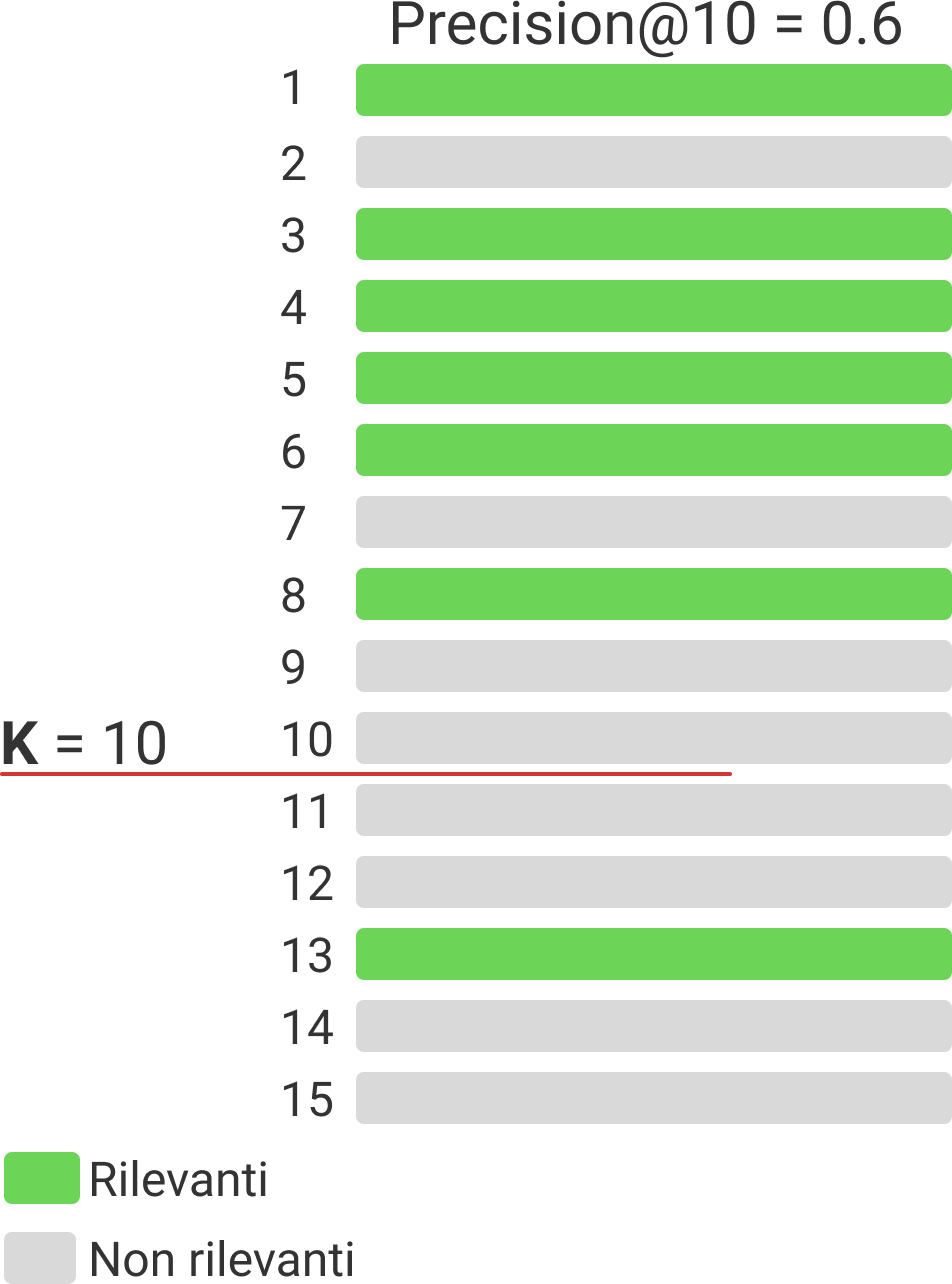
\includegraphics[scale=0.7]{figures/algorithms/precision_@_k.png}
    \caption{L'immagine mostra un esempio di $Precision@10 = 0{.}6$, dove 6 delle 10 raccomandazioni principali risultano \textit{rilevanti} (in verde) e 4 \textit{non rilevanti} (in grigio). La linea rossa evidenzia il cutoff a $K = 10$.}
\end{figure}

Per questo motivo ogni funzione di evaluation all'interno del modulo è stata implementata in due versioni:

\begin{itemize}
    \item funzione normale, con la signature specificata sopra in cui viene chiamata semplicemente la \texttt{predict} del modello
    \item una sua versione \textit{Factory}: questa versione, il cui nome termina con \texttt{\_factory}, riceve in ingresso una funzione \textit{higher order} \texttt{predict\_fn} e le \textit{keyword args} (\texttt{**kwargs}) di \textit{Python}. \texttt{predict\_fn} verrà chiamata all'interno di una nuova funzione costruita dalla \textit{factory} che avrà la \textit{signature} compatibile con i requisiti di \textit{Scikit-learn}. I \textit{keyword args} verranno passati a \texttt{predict\_fn}. Questo serve per poter dare la possibilità di creare funzioni di metriche custom, per esempio dare la possibilità di poter passare features o parametri aggiuntivi per il metodo \texttt{predict}, come nel caso della classe di \texttt{LightFM} che può ricevere le features di \textit{user} e \textit{item}
    \begin{lstlisting}[caption=Implementazione in pseudo codice di una \textit{factory} per una metrica generica ]
        def metric_factory(predict_fn, **kwargs):
            def metric(model, testset, y=None):
                predictions = predict_fn(model, X, **kwargs)
                # metric computation
                result = ...
                return result
            return metric
    \end{lstlisting}
\end{itemize}

Le funzioni di evaluation implicite utilizzano la funzione \\ \texttt{create\_rankings\_from\_implicit} presente nel modulo \texttt{utils} per calcolare il ranking dei \textit{k} migliori \textit{item} per ogni \textit{user} a partire dagli \textit{score} calcolati dal modello.


\section{Utils}

Viene fornita una descrizione più dettagliata delle funzioni presenti nel modulo \texttt{utils}:

\begin{itemize}
    
    \item \texttt{check\_model\_inputs}: controlla che l'input sia dei tipi e nel formato corretto o lancia un \texttt{ValueError}
    \item \texttt{generate\_user\_item\_pairs}: genera tutte le possibili coppie \\ (\textit{user\_id}, \textit{item\_id}) utilizzando la funzione \texttt{itertools.product}
    \item \texttt{create\_rankings\_from\_implicit} / \texttt{create\_rankings\_from\_explicit}: \\ queste funzioni ricevono in ingresso un \textit{DataFrame} o \textit{NumPy array} di coppie \texttt{(user\_id, item\_id)}, una lista di \textit{score} o \textit{rating} e generano una classifica ordinata per ciascun \textit{user} o \textit{item}, a seconda del valore del parametro booleano \texttt{is\_user\_ranking}.
    \begin{itemize}
        \item se \texttt{True}, il ranking è costruito per ciascun \textit{user}, raggruppando tutti gli \textit{item} associati e ordinandoli in base allo \textit{score} (o \textit{rating}) in ordine decrescente
        \item se \texttt{False}, il ranking è costruito per ciascun \textit{item}, raggruppando tutti gli \textit{user} associati e ordinandoli in base allo \textit{score} (o \textit{rating}) in ordine decrescente.
    \end{itemize}
    La funzione restituisce un dizionario in cui:
    \begin{itemize}
        \item le chiavi sono gli \textit{user\_id} oppure di \textit{item\_id}
        \item i valori sono liste ordinate in modo decrescente per \textit{score/rating} di \textit{(item\_id/user\_id, score/rating)}.
    \end{itemize}
\end{itemize}
% \chapter{Valutazione}

Tutto il codice della libreria è stato soggetto a \textit{unit test}, che sono stati eseguiti con il framework \textit{Pytest}. Non sono stati implementati \textit{integration test}, poiché la libreria è progettata per essere utilizzata in modo modulare e le interazioni tra i componenti sono state verificate singolarmente. In aggiunta ai test è stata calcolata la percentuale di \textit{coverage} raggiunta utilizzando il tool \textit{coverage}. In totale la \textit{coverage} raggiunta è del 100\%. Il modulo di \texttt{visualization} è stato testato manualmente, poiché non è possibile automatizzare completamente la verifica dei grafici generati. Tuttavia, sono stati effettuati controlli visivi per garantire che i grafici fossero corretti e rappresentativi dei dati.

\textit{Dataset utilizzati per i test}:

\begin{itemize}
    \item \textit{LovieLens-1M}: esempio classico di dataset per sistemi di raccomandazione, con 1 milione di valutazioni di film da parte degli utenti. Contiene anche features sui film e sugli utenti, come generi, età e sesso
    \item \textit{Retailrocket Dataset}: presente su \textit{Kaggle}, contiene dati di interazioni tra utenti e \textit{item} in un negozio online, con informazioni su visualizzazioni, aggiunte al carrello e acquisti. È utile per testare modelli di raccomandazione basati su interazioni implicite
    \item \textit{dataset interno}: contiene dati di interazioni tra utenti e polizze assicurative. Le features degli utenti includono età, sesso e nazionalità, mentre le polizze hanno informazioni su tipo, durata e costo. È utile per testare modelli di raccomandazione in ambito assicurativo
\end{itemize}

\section{Test preprocessing}

Per il testing dei \textit{transformers} sono stati utilizzati un misto di dataset reali e sintetici. I dataset sintetici sono stati creati per coprire casi d'uso specifici, come la presenza di valori mancanti o la necessità di utilizzare le varie tipologie di \textit{binning}. I dataset reali sono stati utilizzati per verificare che i \textit{transformers} funzionassero correttamente con dati del mondo reale. Ogni \textit{transformer} è stato testato rispetto alle operazioni equivalenti implementate in \textit{Pandas}, \textit{NumPy} e \textit{Scikit-learn}. I risultati sono stati confrontati per garantire che la libreria producesse gli stessi output. Per i \textit{transformers} che utilizzano possibili modalità come parametri di input (e.g. \texttt{FillNa} con il campo \texttt{method}) sono state usate singole liste o l'oggetto \texttt{ParameterGrid} di \textit{Scikit-learn} per generare tutte le combinazioni possibili di parametri.

\section{Test modelli}

Per i modelli l'obbiettivo dei test è stato in primis di verificare che i modelli fossero compatibili con la libreria \textit{Scikit-learn}. Questa verifica è stata possibile grazie alla funzione \texttt{check\_estimator} di \textit{Scikit-learn}, che ha permesso di testare i modelli rispetto a un insieme di casi d'uso standardizzati. Successivamente, si è proceduto a testare i modelli rispetto al formato dei dati in ingresso e in uscita, per garantire che i modelli potessero essere utilizzati con il formato standard. Infine si è verificato che ciascun modello riproducesse le stesse predizioni dei modelli delle librerie originali a parità di configurazione. Tutti i test sono stati eseguiti utilizzando i dataset di test descritti in precedenza. Per il modello di \textit{LightFM} sono state testate tutte le combinazioni che in includevano o escludevano le features degli utenti e dei \textit{item}.

Per i modelli che implementano \texttt{similar\_items} e \texttt{similar\_users}:

\begin{itemize}
    \item per i modelli di \textit{Implicit} si è fatto un confronto con i metodi della libreria originale, verificando che i risultati fossero equivalenti
    \item per il modello \textit{LightFM} e i modelli di \textit{Surprise} si è verificato che i risultati fossero equivalenti a quelli ottenuti eseguendo il calcolo della similarità \texttt{cosine\_similarity} di \textit{Scikit-learn} o, nel caso specifico del modello \textit{KNNBaseline}, ai risultati ottenuti dalle funzioni di similarità \\ \texttt{surprise.similarities.pearson} \\ o  \texttt{surprise.similarities.pearson\_baseline} e \\ \texttt{surprise.similarities.msd} di \textit{Surprise}
\end{itemize}

Per testare le varie combinazioni di parametri si è utilizzato l'oggetto \\ \texttt{ParameterGrid} di \textit{Scikit-learn}, che permette di generare tutte le combinazioni possibili di parametri per i modelli. Importante sottolineare che alcuni modelli, soprattutto quelli più complessi come \texttt{SVD++}, richiedono un tempo di addestramento significativo, che può variare da pochi secondi a diversi minuti a seconda della configurazione e del dataset utilizzato. Inoltre bisogna considerare che i modelli delle librerie non godono di ottimizzazioni su \textit{GPU} e la libreria \textit{Surprise} nemmeno di ottimizzazioni \textit{Cython} il che la rende lenta nelle fasi di addestramento e predizione. 

\section{Test evaluation}

Per il modulo di \textit{evaluation} sono stati implementati confrontando il valore della metrica rispetto al valore calcolato in modo grezzo, senza l'utilizzo della libreria. In questo modo si è verificato che le metriche calcolate dalla libreria fossero corrette e coerenti con i risultati attesi. Sono state testate anche le metriche per feedback implicito nella loro versione \textit{Factory} con il modello \textit{LightFM}. Le metriche per feedback esplicito in versione \textit{Factory} sono state testate utilizzando come parametro \texttt{predict\_fn} quella base dei modelli di \textit{Surprise} perché non esiste un modello per dati espliciti che potrebbe necessitare di modifiche custom alla metrica. Importante sottolineare che il tempo di calcolo delle metriche dipende sia dalla velocità di predizione del modello sia dalla dimensione del dataset di test. Inoltre, per le metriche implicite la predizione per ciascun utente viene calcolata su tutto l'insieme di \textit{item}, il che può richiedere un tempo significativo, soprattutto per modelli complessi e dataset di grandi dimensioni.

\section{Test altri moduli}
Per tutte le funzioni presenti nei moduli di \texttt{utils} e \texttt{model\_selection} sono state implementate dalle due alle tre funzioni di test sufficienti per coprire i vari casi d'uso.

\section{Usabilità}
La libreria, un volta completata, è stata testata da un gruppo di utenti interni all'azienda \textit{Data Reply} per valutarne l'usabilità e l'efficacia, soprattutto rispetto alle librerie già esistenti ed utilizzate. I feedback raccolti sono stati utilizzati per apportare miglioramenti e ottimizzazioni alla libreria. Si consideri la differenza di linee di codice tra un utilizzo completo di \textit{LightFM} e l'utilizzo della libreria non includendo il preprocessing dei dati:

\begin{lstlisting}[caption=esempio di utilizzo completo della libreria \textit{LightFM}]
RANDOM_STATE = 1234
K = 10
EPOCHS = 100

# train and predict recommendations using original LightFM model
lightfm_model = lightfm.LightFM(random_state=RANDOM_STATE)
# fit Dataset based on features and data
lightfm_dataset = Dataset()
item_features_data = unique(list([(row['item_id'], f"{col}:{value[col]}") 
                                  for _, value in policies_item.iterrows() 
                                  for col in ['duration', 'cost']]))
user_features_data = unique(list([(row['user_id'], f"{col}:{row[col]}")
                                  for _, row in policies_users.iterrows() 
                                  for col in ['age', 'sex', 'nationality']]))

lightfm_dataset.fit(users=unique(policies_users['user_id']),
                    items=unique(policies_users['item_id']),
                    item_features=item_features_data,
                    user_features=user_features_data)

# create interactions matrix and weights matrix instance for data
interactions, weights = lightfm_dataset.build_interactions(trainset.values)

# train the model with features
lightfm_model.fit(interactions,
                  sample_weight=weights,
                  item_features=item_features,
                  user_features=user_features,
                  epochs=EPOCHS)

# get mapping
user_id_mapping, _, item_id_mapping, _ = lightfm_dataset.mapping()

# creates all ids for prediction
predictions_user_ids = np.array([user_id_mapping[user] 
                                 for user in testset['user_id']])
unchanged_user_ids = [user for user, _ in id_pairs]
predictions_item_ids = np.array([item_id_mapping[item] 
                                 for item in testset['item_id']])
unchanged_item_ids = [item for _, item in id_pairs]

# prediction using LightFM model
lightfm_scores = lightfm_model.predict(predictions_user_ids,
                                       predictions_item_ids,
                                       item_features=item_features,
                                       user_features=user_features)
# zip together unchanged ids and predictions scores
total_prediction = [{'user_id': user_id, 'item_id': item_id, 'interaction_weight': score}
                    for user_id, item_id, score in zip(unchanged_user_ids, unchanged_item_ids,lightfm_scores)]
sort_function = lambda x: (x['interaction_weight'], x['item_id'])
map_function =


def select_predictions(grouped_predictions):
    # sort predictions by ranking
    sorted_predictions = sorted(grouped_predictions, 
                                key=lambda x: (x['interaction_weight'], x['item_id']), 
                                reverse=True)
    # select first k
    k_predictions = sorted_predictions[:K]
    # extract only ids
    mapped_predictions = map(lambda x: x['item_id'], k_predictions)
    return list(mapped_predictions)

# compute groups
groups = {key_id: group for key_id, group in 
          groupby(predictions, lambda x: x['user_id']).items()}

# group by key, and extract for each id top k predictions
rankings = {key_id: select_predictions(grouped_predictions)
            for key_id, grouped_predictions in groups.items()}
\end{lstlisting}

\begin{lstlisting}[caption=esempio di utilizzo del modello \texttt{LightFM} libreria]
RANDOM_STATE = 1234
K = 10
EPOCHS = 100

# create model
new_lightfm_model = LightFM(random_state=RANDOM_STATE)
# train model with
new_lightfm_model.fit(trainset, 
                      item_features=item_features,
                      user_features=user_features, 
                      epochs=EPOCHS)
# create predictions
new_total_prediction = new_lightfm_model.predict(testset, 
                                                 user_features=user_features,
                                                 item_features=item_features)
# create rankings from predictions
new_rankings = create_rankings_from_implicit(dataset=testset,
                                             scores=new_total_prediction, 
                                             k=K, 
                                             is_user_ranking=True)
\end{lstlisting}

Come si può notare, l'utilizzo della libreria consente di ridurre significativamente il numero di linee di codice necessarie per addestrare e utilizzare un modello di \textit{LightFM}, rendendo il codice più leggibile e mantenibile.

\section{Documentazione}
Per garantire la facilità d'uso della libreria, è stata creata una documentazione completa utilizzando \textit{Sphinx} utilizzando il tema \texttt{sphinx\_rtd\_theme}. La documentazione include:

\begin{itemize}
    \item una guida all'installazione e all'utilizzo della libreria
    \item una descrizione dettagliata di ogni modulo e delle sue funzioni
    \item esempi di utilizzo per ciascun modulo
\end{itemize}

\section{CI/CD}

Per garantire la qualità del codice e l'affidabilità della libreria, è stato implementato un sistema di \textit{Continuous Integration/Continuous Deployment} (\textit{CI/CD}) utilizzando la \textit{GitHub Actions} \texttt{astral-sh/setup-uv@v5} per la gestione del tool \textit{uv}. Questo sistema esegue automaticamente i test ogni volta che viene effettuata una modifica con versione del codice, notificando con una mail in caso di fallimento. Si è deciso di utilizzare l'esecuzione dei test solamente per modifiche significative in quanto il tempo di esecuzione dei test è elevato. Inoltre, ha il compito di generare la documentazione della libreria e di pubblicarla su \textit{GitHub pages} e su \textit{Confluence} utilizzando un'integrazione ad hoc.

\section{Limiti della soluzione proposta}




% \chapter{Conclusioni e Lavori Futuri}\label{conclusioni-e-lavori-futuri}


%----------------------------------------------------------------------------------------
% BIBLIOGRAPHY
%----------------------------------------------------------------------------------------

\backmatter

\nocite{*} % Remove this as soon as you have the first citation

\bibliographystyle{alpha}
\bibliography{bibliography}

\begin{acknowledgements} % this is optional
Optional. Max 1 page.
\end{acknowledgements}

\end{document}
